\chapter{Charged Higgs Search}
\label{chargedH}
\begin{chapabstract}
A search for evidence of the charged Higgs boson from LHC collisions is 
presented in this chapter. Potential charged Higgs boson masses were scanned from 200 
to 2000~\GeV. Observations in this data-set indicate that it is consistent with the Standard 
Model predictions, rather than predictions from the hMSSM. Exclusion limits were 
set on the production cross section of the charged 
Higgs boson times the branching ratio of its decay to a $\tau$ lepton and a $\tau$ neutrino.  
In Section~\ref{sec:samplesCh} the data-sets used in the search are presented. Data obtained from 
LHC collisions is referred to as {\it data}, while data obtained from simulation is just referred to 
as {\it simulation}. In Section~\ref{sec:objCh} physics object selection criteria are presented, adding to the 
 criteria presented in Chapter~\ref{obj}. In Section~\ref{sec:evSelCh} the 
criteria to select events with a charged Higgs boson 
signature are introduced. Treatment of backgrounds to the charged Higgs boson is discussed in 
Section~\ref{sec:bkgCh}, with the associated systematic uncertainties discussed in Section~\ref{sec:systsCh}. 
Final event yields are presented in Section~\ref{sec:resCh}, and their statistical assessment is 
discussed in the same section.
% It should be acknowledged that the treatment of background processes was 
%a collaborative effort, of which the author is proud to have contributed significantly.   
\end{chapabstract}

\section{Data and Simulation}
\label{sec:samplesCh}
\par Data used for this analysis was collected by the ATLAS detector during Run II 
of the LHC. The LHC parameters and conditions during this data-taking period are discussed 
in Chapter~\ref{expSetup}. Only data from runs during which proton beams were stable\footnote{Stable beams 
are those that have a stable energy of 6.5~\TeV.} were considered. 
The total integrated luminosity of this data-set is 14.7~\ifb, 3.2~\ifb\ of 
which was collected in 2015. The rest was collected in 2016. Uncertainties on the 2016 
and 2015 luminosities were 3.7\% and 2.1\% respectively. The impact of these uncertainties on the 
final results of this search is discussed in Section~\ref{sec:resCh}. 

\par Expected signal and background events were computed using Monte Carlo (MC) simulation, 
as discussed in detail in Chapter~\ref{sim}. 
%Ingredients for such simulations are 
%\begin{enumerate}
%\item a hard scatter event generator;
%\item a set of parton density functions (PDFs) that describe momentum distributions of gluons and quarks 
%in the proton; 
%\item an underlying event generator that is tuned to match conditions during data-taking period;
%\item and models for parton showering, fragmentation and hadronization that are also tuned to match real data. 
%\end{enumerate} 
%
As discussed in Section~\ref{sec:cHtheory}, 
for high \mcH\ the charged Higgs boson is produced in association with a top quark. Such a production mode 
is dominated by the 4FS and 5FS diagrams shown in Figure~\ref{fig:chargedFeynV1}.
 Since the 4FS and 5FS diagrams have similar topologies~\cite{Flechl:2014wfa},  
without loss of generality signal samples were generated only from the 4FS diagram. 
Using the NNPDF23LO~\cite{Ball:2012cx} PDF set, hard scatter 
events were generated by \MGMCatNLO~\cite{Alwall:2014hca} version 2.2.2.
Underlying events were generated by \PYTHIA8~\cite{Pythia8} version 8.186,
 whose parameters were tuned to match parameters, 
called A14~\cite{ATL-PHYS-PUB-2014-021}, observed in data. 
Parton showering, fragmentation and hadronization were handled 
by \PYTHIA~\cite{Sjostrand:2000wi} version 6.428. 
Taking the mass of the top quark as $172.5~\GeV$,  
18 signal samples with $200~\GeV\leq\mcH\leq2000~\GeV$ were independently generated.   

\begin{figure}[!h]
\centering
\begin{subfigure}{0.4\textwidth}
   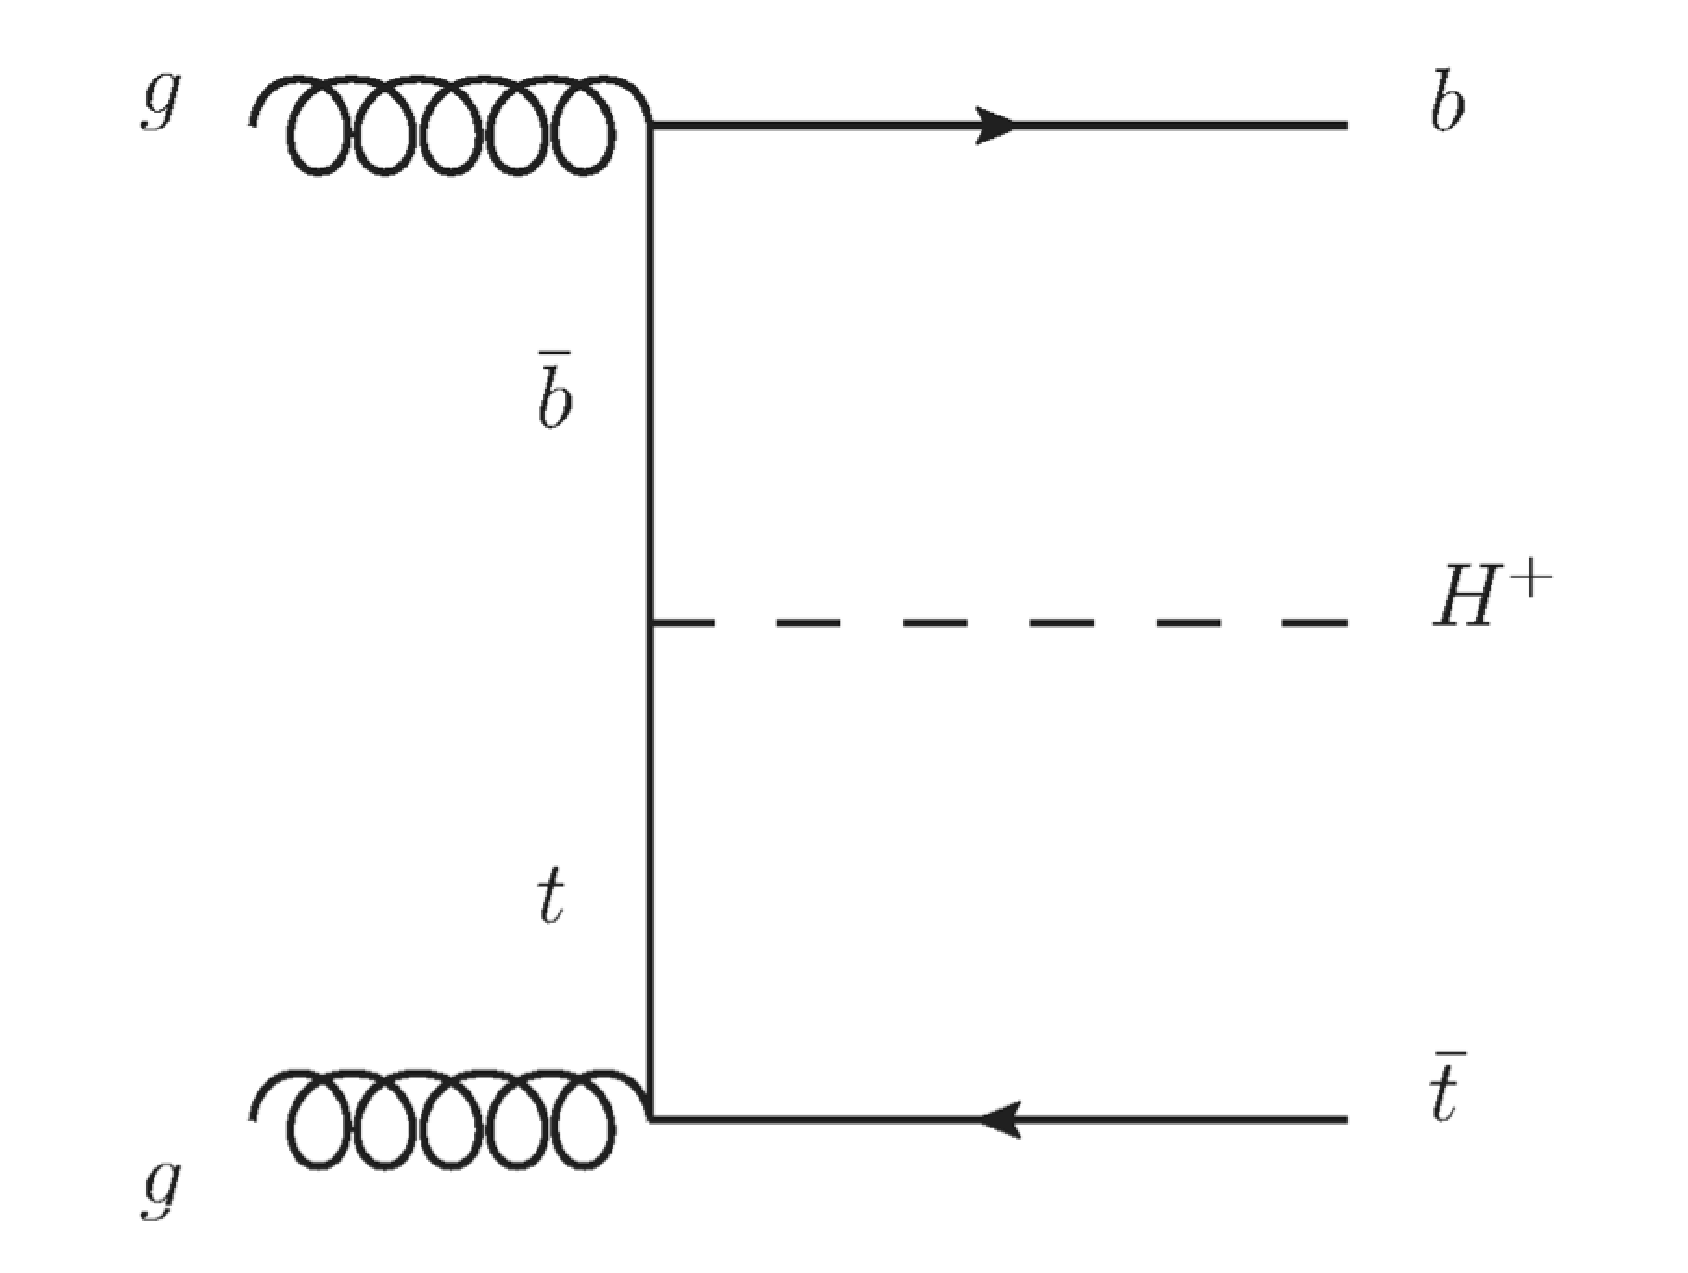
\includegraphics[width=\textwidth]{figures/feynmanIIIa.eps}
\caption{Top association -- 4FS}
\end{subfigure} % 
\begin{subfigure}{0.4\textwidth}
   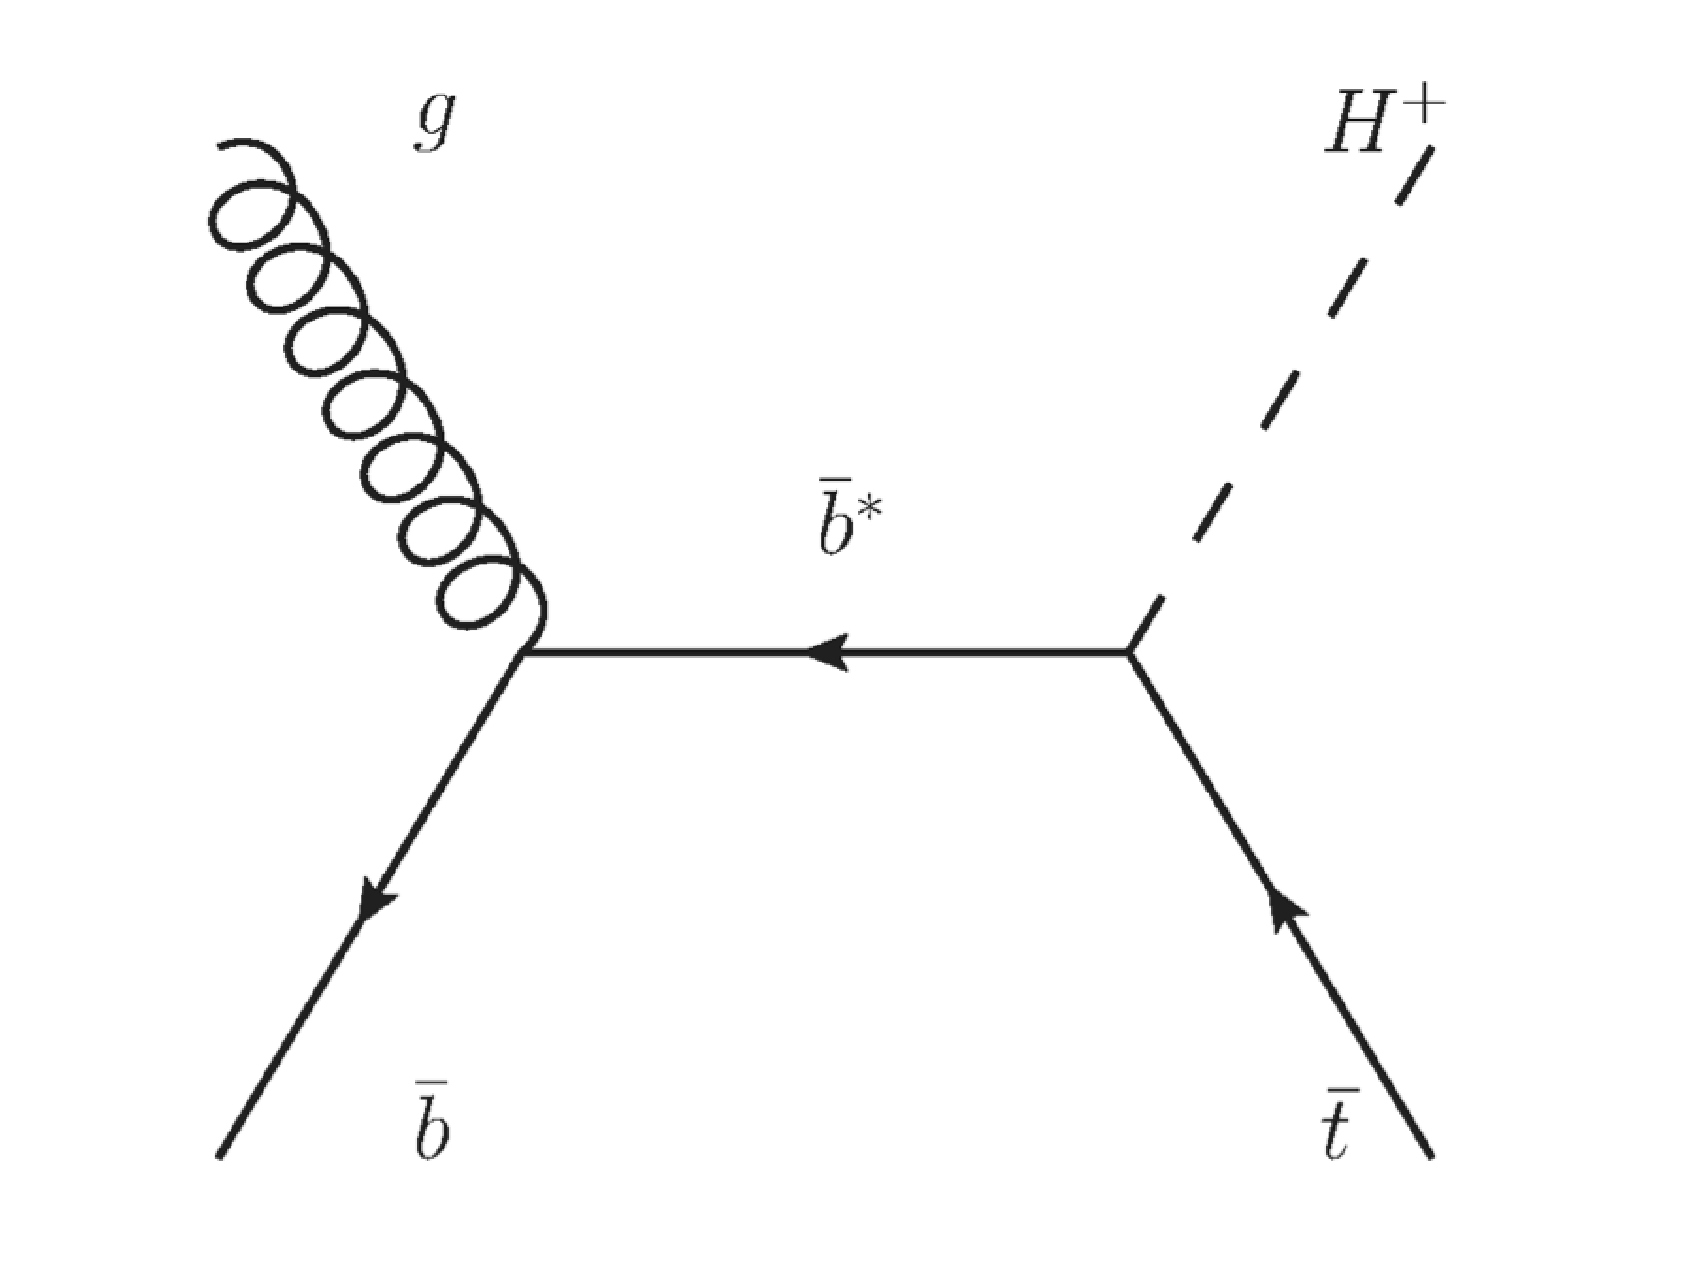
\includegraphics[width=\textwidth]{figures/feynmanIIa.eps}
\caption{Top association -- 5FS}
\end{subfigure} %
\caption{Leading order Feynman diagrams for the charged Higgs boson production}
\label{fig:chargedFeynV1}
\end{figure}

\par The \ttbar\ process, shown in Figure~\ref{fig:ttBarDg}, is the most dominant process 
with a top quark in the final state at the 
LHC~\cite{Aad:2015eia}. It is therefore expected to be the most dominant background to the charged Higgs boson 
produced in association with a top quark.
The next dominant source of top quarks at the LHC is the {\it single top} process, 
produced through any of the $\operatorname{s-,t-}$ or $\operatorname{Wt-}$channels shown in Figure~\ref{fig:singleTopDg}.
The hard scatter events for \ttbar, $\operatorname{Wt-}$ and $\operatorname{s-}$channel single top processes 
were generated by \POWHEG-\textsc{Box}~\cite{PowhegBox, Alioli:2008tz,Powheg0,Powheg1,Powheg2} version 2
 at NLO, using the CT10~\cite{Lai:2010vv, Gao:2013xoa} PDF set.  
\POWHEG-\textsc{Box} version 1 was used to generate the $\operatorname{t-}$channel single top hard scatter event, 
using the CT10F4\footnote{The `F4' indicates that this is a 4FS version of the standard CT10 PDF set}
 PDF set. Again, the mass of the top quark was set at $172.5~\GeV$. 
Using the CTEQ6L1~\cite{Nadolsky:2008zw} PDF set \PYTHIA\ version 6.428 was used to model parton showering, 
fragmentation and the underlying event. These models were tuned with the Perugia 2012~\cite{Skands:2010ak} parameters. 
While the \ttbar\ cross section was calculated to NNLO+NNLL, 
single top processes were normalized to NNLO cross sections.   

\par \ttbar\ and single top processes are collectively referred to in this search 
as {\it Top}.\footnote{Not to be confused with the {\it top} quark, which will either be 
in full small caps, or abbreviated to $t$.}

\begin{figure}[h]
   \includegraphics[width=.5\textwidth]{figures/feynman_ttbar_LHC_gggtt.png}
   \includegraphics[width=.5\textwidth]{figures/feynman_ttbar_LHC_ggttt.png}
\caption{Leading order Feynman diagrams for \ttbar\ production at the LHC. Taken from 
Ref~\cite{D0:ttBarFeyn}}
\label{fig:ttBarDg}
\end{figure} % 

\begin{figure}[h]
\begin{subfigure}{0.33\textwidth}
					 \includegraphics[width=\textwidth]{figures/feynman_tb_bold_ltblue_whitebkgd.png}
\caption{$\operatorname{s-}$channel}
\end{subfigure}%  
\begin{subfigure}{0.33\textwidth}
					 \includegraphics[width=\textwidth]{figures/feynman_tq_bold_midblue.png}
\caption{$\operatorname{t-}$channel}
\end{subfigure}%
\begin{subfigure}{0.33\textwidth}
					 \includegraphics[width=\textwidth]{figures/feynman_tqb_bb_bold_midblue.png}
\caption{$\operatorname{Wt-}$channel}
\end{subfigure}%
\caption{Leading order Feynman diagrams for single top quark production at the LHC. Taken 
from Ref~\cite{D0:ttBarFeyn}} 
\label{fig:singleTopDg}
\end{figure} % 

\par Events containing a $W$ or \Zboson\ boson and some associated jets are 
also expected to be a significant background to the signal. Their hard scatter events were generated by 
\MGMCatNLO\ version 2.2.2 with the NNPDF23LO PDF set. \PYTHIA8\ was used to generate 
the underlying events, while \PHOTOS~\cite{Davidson:2010ew} was used to radiate photons from charged leptons. 
All the cross sections were normalized to NNLO. 

\par Events with two vector bosons and associated
jets, referred to collectively as {\it VV} or {\it Diboson}, were generated by \POWHEG-\textsc{Box} version 2 interfaced 
with \PYTHIA\ version 8.186 for the parton shower models. The CT10 PDF set was used to model 
gluon and quark momenta in the protons. Cross sections were normalized to NLO. 

\par Bottom and charm quark decays were produced and decayed by \textsc{Evtgen}~\cite{Lange2001152}
 version 1.2.0. Pileup events were added to these 
events with \PYTHIA\ version 8 using the MSTW2008LO~\cite{Martin:2009iq, Martin:2009bu, Martin:2010db}
 PDF set. Just like in signal, parton showering, hadronization and fragmentation models in \PYTHIA\ version 8 were 
also tuned with the A14 parameter set.  


\section{Object Selection}
\label{sec:objCh}
\par Physics objects used in this search are jets, hadronic $\tau$ leptons, electrons, 
muons and missing transverse energy. Reconstruction and identification of these objects 
from detector signals is discussed in detail in Chapter~\ref{obj}. This section summarizes other 
selection criteria imposed on these physics objects, specific to this analysis. 

\par Basic jet reconstruction is discussed in Section~\ref{sec:jets}. Of the  
jets that were reconstructed using the anti-$k_T$ algorithm with $\Delta R=0.4$, only those 
with $\pT>25~\GeV$ and $|\eta|<2.5$ were considered. For jets with $\pT<60~\GeV$, the Jet Vertex 
Tagger (JVT) was used to reduce effects from pileup events. The $\operatorname{b-}$tagging algorithm 
described in Section~\ref{sec:bTag} was applied on each jet that passed this selection criteria, ultimately 
assigning to it a {\it $\operatorname{b-}$tagging score}. The working point for the score used to identify $\operatorname{b-}$tagged 
jets in this analysis corresponds to a 70\% efficiency in identifying $\operatorname{b-}$jets 
in \ttbar events, at a background rejection rate of 400.   

\par Primary reconstruction of hadronic $\tau$ leptons is discussed in Section~\ref{sec:tau}. 
Since every hadronic $\tau$ decay includes a $\nu_\tau$ in its final state, the reconstruction 
was performed only on the visible components of the decay products. The reconstructed object, which 
estimates the $\tau$ lepton, is referred to here as a \tauvis.   
Treatment of $\tauvis$ was separated into 1-prong and 3-prong candidates, corresponding to decays 
to 1 $\pipm$ or 3 $\pipm$ respectively.  A boosted decision 
tree (BDT) was trained to distinguish $\tauvis$ candidates from jets initiated by quarks or gluons. 
Loose and medium working points on the BDT output were used for different purposes in this search. 
The loose working point corresponds to 70\% and 65\% identification efficiencies on the 1-prong and 3-prong 
$\tauvis$ candidates. The medium working point corresponds to 55\% and 40\% identification efficiencies on 
the 1-prong and 3-prong $\tauvis$ candidates. In both cases, the background rejection rate 
was found to be of $\mathcal{O}(10^2)$. All $\tauvis$ candidates were required to have $\pt>40~\GeV$ and $|\eta|<2.3$. 

\par Electron and muon reconstruction and identification is discussed in detail in Sections~\ref{sec:ele} and 
\ref{sec:mu}. Loosely identified and loosely isolated electrons were selected. To further ensure that the electrons originated 
from the primary vertex, $|z_0\sin\theta|<0.5$ and $|d_0/\sigma_{d_0}|<5$ we imposed.  
Electron candidates that satisfied these selection criteria were additionally required 
to have $\pt>20~\GeV$, and be within $|\eta|<2.47$, excluding transition between the barrel and end-cap regions $1.37<|\eta|<1.52$.
Muons were also loosely identified and isolated. In addition, impact parameter selection 
criteria were imposed on them to ensure that they originated from the primary 
vertex: $|z_0\sin\theta|<0.5$ and $|d_0/\sigma_{d_0}|<3$. 
Those that satisfied these requirements were required to have $\pt>20~\GeV$ and be within $|\eta|<2.5$.  

\par Overlap between the physics objects discussed above were resolved using the following priority list: 
$\mu\to e\to\tauvis\to\text{jet}$. If an electron was found within $\Delta R < 0.2$ 
of a reconstructed muon, the electron was removed from the list of physics objects in that event. This is 
because since electrons experience photon radiation and brehmsstrahlung at a higher rate than muons, they are   
more difficult to reconstruct. If a $\tauvis$ was reconstructed within $\Delta R<0.2$ of an electron 
or muon, the $\tauvis$ was removed. Likewise, if a jet was reconstructed within $\Delta R<0.2$ of an electron, muon 
or $\tau$ lepton, the jet was removed from the list.   

\par \met, the magnitude of the missing transverse momentum, was reconstructed after all 
the other physics objects were identified and overlaps were resolved. 
It was reconstructed as the negative vector sum of all the reconstructed and calibrated objects, and the reconstructed 
tracks that were not associated to any physics objects. All these objects were required to originate from the hard 
scatter event. This association with the hard scatter event reduced effects from pileup events on the reconstructed 
\met.

\par Table~\ref{tab:objcH} summarizes all the physics object selection criteria for this analysis.     

\begin{table}[!h]
\centering
  \resizebox{\textwidth}{!}{
   \begin{tabular}{|l|c|}
\hline
 Physics Object           								& Selection Criteria \\
\hline\hline
 \multirow{3}{*}{Jets}  & anti-$k_T$ with $\Delta R=0.4$ \\
			& $\pT>25~\GeV$, $|\eta|<2.5$    \\
			& JVT for $\pt<60~\GeV$ \\
\hline 
$b$-tagged Jets & $b$-tagging score at 70\% efficiency working point \\
\hline
  \multirow{3}{*}{\tauvis} & BDT score working point at 55\%(40\%) efficiency for 1(3)-prong for medium \\
 				& BDT score working point at 70\%(65\%) efficiency for 1(3)-prong for loose \\
				& $\pT>40~\GeV$, $|\eta|<2.3$ \\
\hline  
  \multirow{3}{*}{Electrons} & Loose ID \\
					& Loose Isolation \\
					& $\pT>20~\GeV$, $|\eta|<2.47$ excluding $1.37<|\eta|<1.52$ \\
\hline
  \multirow{3}{*}{Muons}     & Loose ID \\
					& Loose Isolation \\
					& $\pT>20~\GeV$, $|\eta|<2.5$ \\
\hline 
   \end{tabular}
}
\caption{Selection criteria for physics objects.}
\label{tab:objcH}
\end{table}


\section{Event Selection}
\label{sec:evSelCh}
\par Evidence for the charged Higgs boson was searched for in events in which the Higgs boson 
decays to a $\tau$ lepton and a $\nu_\tau$. In these events, the $\tau$ lepton decays hadronically 
and is reconstructed as a $\tauvis$. The 4FS and 5FS topologies for such events, signal events, are 
respectively  

\begin{equation}
gb\to[t][H^+]\to[(jj)b][(\tauvis+\met)]
\label{eq:topA}
\end{equation} 
and 
\begin{equation}
gg\to[tb][H^+]\to[(jj)bb][(\tauvis+\met)].
\label{eq:topB}
\end{equation}

In the terminology of Equations~\ref{eq:topA} and~\ref{eq:topB} a $b$-tagged reconstructed jet 
is represented by $b$, otherwise it is represented by $j$. 
Table~\ref{tab:sigReg} summarizes the selection criteria optimized to select signal events as represented by 
 Equations~\ref{eq:topA} and~\ref{eq:topB} and minimize the level of background contamination. These 
selection criteria define the {\it signal region}. This section 
discusses each component of these selection criteria.  

\par Before pre-selection, measures were taken to reduce the number of events originating 
from instrumental effects such as intra-beam interactions and proton losses upstream of the 
interaction point.\footnote{Proton losses from the beam may induce cascades that may 
eventually reach the ATLAS detector. These cascades would be reconstructed as jets.} 
 This was achieved by requiring the following :

\begin{enumerate}
\item no jet with $\pT>25~\GeV$ that fails 
the \texttt{BadLoose} quality selection criteria discussed in Section~\ref{sec:jets}; 
\item at least one vertex with two or more tracks. This selection is designed to identify the primary 
vertex to which all the physics objects should point; 
\item the SCT, Tile and LAr Calorimeters not be in an error or unknown state; 
\item and the event must be considered {\it complete} by the TTC.\footnote{See Section~\ref{sec:trigger} 
for a more formal definition of `complete'.}
\end{enumerate}

These selection criteria are collectively referred to as {\it clean-event} in the rest of 
this chapter. 

\begin{table}[!h]
\centering
  \resizebox{\textwidth}{!}{
   \begin{tabular}{|l|r|}
\hline
            								& Selection \\
\hline\hline
\multirow{4}{*}{pre-selection}& Pass trigger \texttt{HLT\_xe70\_tc\_lcw}(\texttt{HLT\_xe90\_mht}) for 2015(2016) data \\
															& Exactly one $\tauvis$ with $\pt>40$~\GeV \\ 
															& At least 3 jets with $\pt>25$~\GeV \\
															& No muon or electron \\ 
\hline
\multirow{3}{*}{full selection} & At least one $b-$tagged jet \\				
																& $\met>150$ GeV \\
																& $\mT>50$ GeV \\
\hline 
   \end{tabular}
}
\caption{Signal region definition. Additionally, measures were taken to ensure that events originated 
from inelastic $pp$ collisions and no jets originated from unwanted experimental effects.}
\label{tab:sigReg}
\end{table}

\par The event topology presented in Equations~\ref{eq:topA} and~\ref{eq:topB} suggests several options 
to trigger on when selecting such events. One could use a trigger that demands presence of a $\tauvis$, some \met, 
or both the $\tauvis$ and some $\met$. The least stringent $\tauvis$-only trigger available on both the 
2015 and 2016 trigger menu required presence of a $\tauvis$ with $\pT>160~\GeV$ in the event. Since the topology 
in Equations~\ref{eq:topA} and~\ref{eq:topB} is not biased towards high-\pt\ $\tau$ leptons, a $\tauvis$-only 
trigger was not chosen. The least stringent of all unprescaled triggers that require presence of both a $\tauvis$ 
and some $\met$ required the $\tauvis$ to have at least 35~\GeV\ in \pt\ and $\met>70~\GeV$. Likewise, the least stringent 
unprescaled trigger that requires the presence of just \met\ required $\met>70~\GeV$. The efficiencies of the \met-only and 
the \met+\tauvis\ triggers when selecting signal events in Monte Carlo simulation were found to be comparable. Thus, there was 
no advantage in using an \met+\tauvis\ trigger over an \met-only trigger. 

\par To avoid imposing selection criteria on the \tauvis, only \met-only-based triggers were considered.  
Figure~\ref{fig:trigComp} shows signal selection efficiency distributions for several of \met-only triggers 
on a signal sample with $\mcH=200$~\GeV, binned in \met. The naming convention for these triggers can be  
generalized to
\begin{center}
 \texttt{Level\_xeMissingEnergyCut\_MissingEnergyReco}.
\end{center}
\texttt{Level} indicates the level in the trigger 
system at which the trigger is active. In this case, the level is \texttt{HLT}, denoting the Higher Level Trigger. At 
this level the \met\ may be reconstructed using either topological clusters, in which case 
\texttt{MissingEnergyReco} is \texttt{tc\_lcw}, or jet energies, in which case  
\texttt{MissingEnergyReco} is \texttt{mht}. Otherwise, the \met\ is reconstructed using energy recorded in 
calorimeter cells. For $100<\met<200$~\GeV, 
the most efficient trigger is \texttt{HLT\_xe70\_tc\_lcw}, which accepts events with $\met>70$~\GeV. 

\begin{figure}[!h]
\centering
   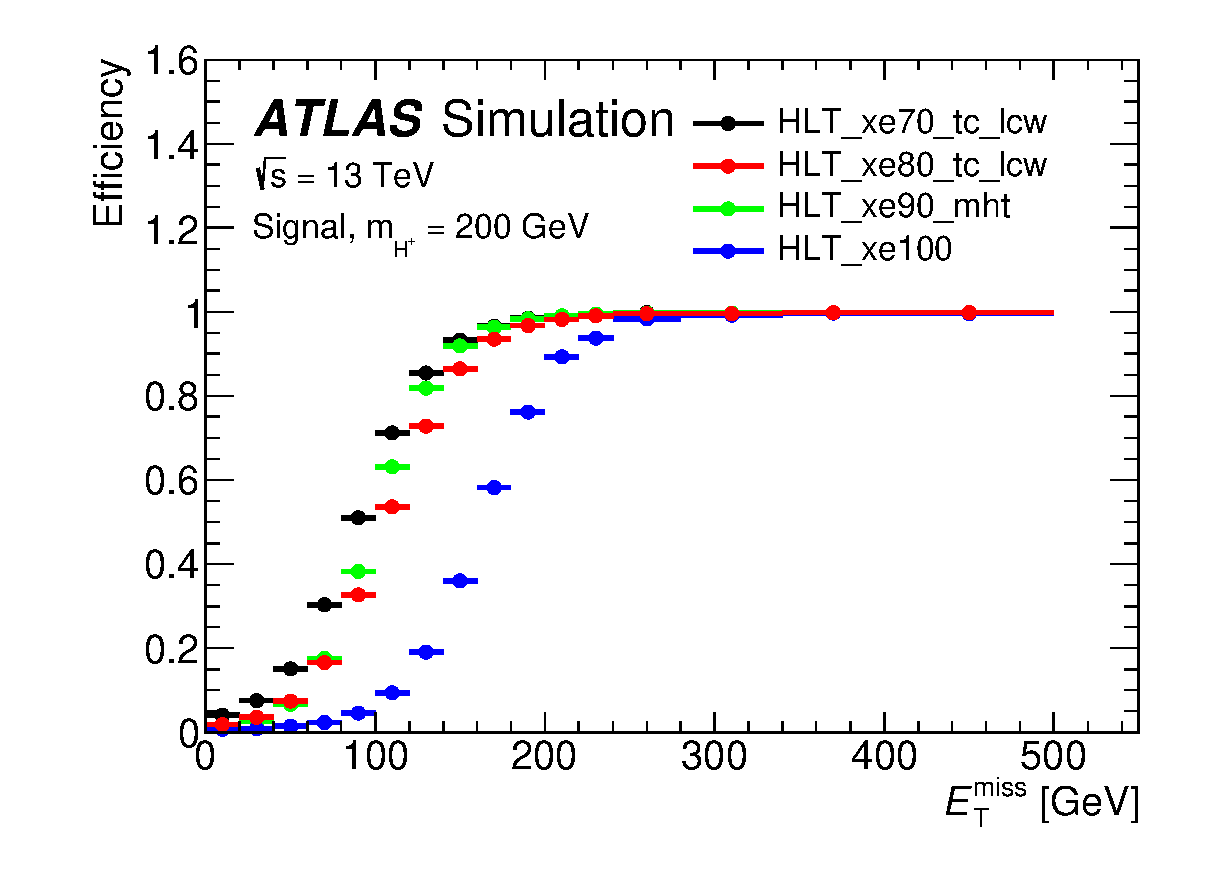
\includegraphics[width=0.8\textwidth]{figures/mh200_xe70_xe90_xe100_xe80.eps}
\caption{Plots of the efficiencies of several \met-based triggers, obtained from simulation of signal with $\mcH=200~\GeV$}
\label{fig:trigComp}
\end{figure}
 
\par While \texttt{HLT\_xe70\_tc\_lcw} was the least stringent \met-only trigger during the 2015 data-taking period, 
\texttt{HLT\_xe90\_mht} was the least stringent in the 2016 data-taking period. 
Events from the 2015 data-set were therefore triggered with \texttt{HLT\_xe70\_tc\_lcw}, and events from the 
2016 data-set were triggered with \texttt{HLT\_xe90\_mht}.
 
\par In addition to trigger requirements, the pre-selection criteria required  
events to have exactly one $\tauvis$. The said \tauvis\ was also required to have $\pt>40$~\GeV. 
At least 3 reconstructed jets with $\pt>25$~\GeV\ were required to be present. 
Since the topologies in Equations~\ref{eq:topA} and ~\ref{eq:topB} do 
not include electrons or muons, the event was also required to have no electrons or muons.  

\par For the full selection at least one $b-$tagged jet was demanded. Additionally, the event had 
to have $\met>150$~\GeV\ and
 $\mT>50$~\GeV, where \mT\ is the transverse mass of the $\tauvis,\met$ system :

\begin{equation}
\mT = \sqrt{2\pt^\tau\met(1-\cos\Delta\phi_{\tau,\met})}.
\end{equation} 

Figures~\ref{fig:preselectA} and~\ref{fig:preselectB} show expected $\met$ and $\mT$ `n-1'
 distributions after the full selection criteria has been applied,\footnote{These are distributions where 
all the selection criteria has been applied except the criteria based on the variable being plotted.} 
for backgrounds where the $\tauvis$ was reconstructed from a $\tau$ lepton and for 
several signal samples. Vertical black lines show the point at which \met\ and \mT\ are cut 
on. As already been predicted, it is expected that the Top background dominates, followed by the 
\Wjets\ background.

\par Treatment of backgrounds where the \tauvis\ is reconstructed from objects other 
than $\tau$ leptons is discussed in Sections~\ref{sec:jetToTau} and \ref{sec:lepToTau}.    

\begin{figure}[!h]
\begin{subfigure}{0.5\textwidth}
   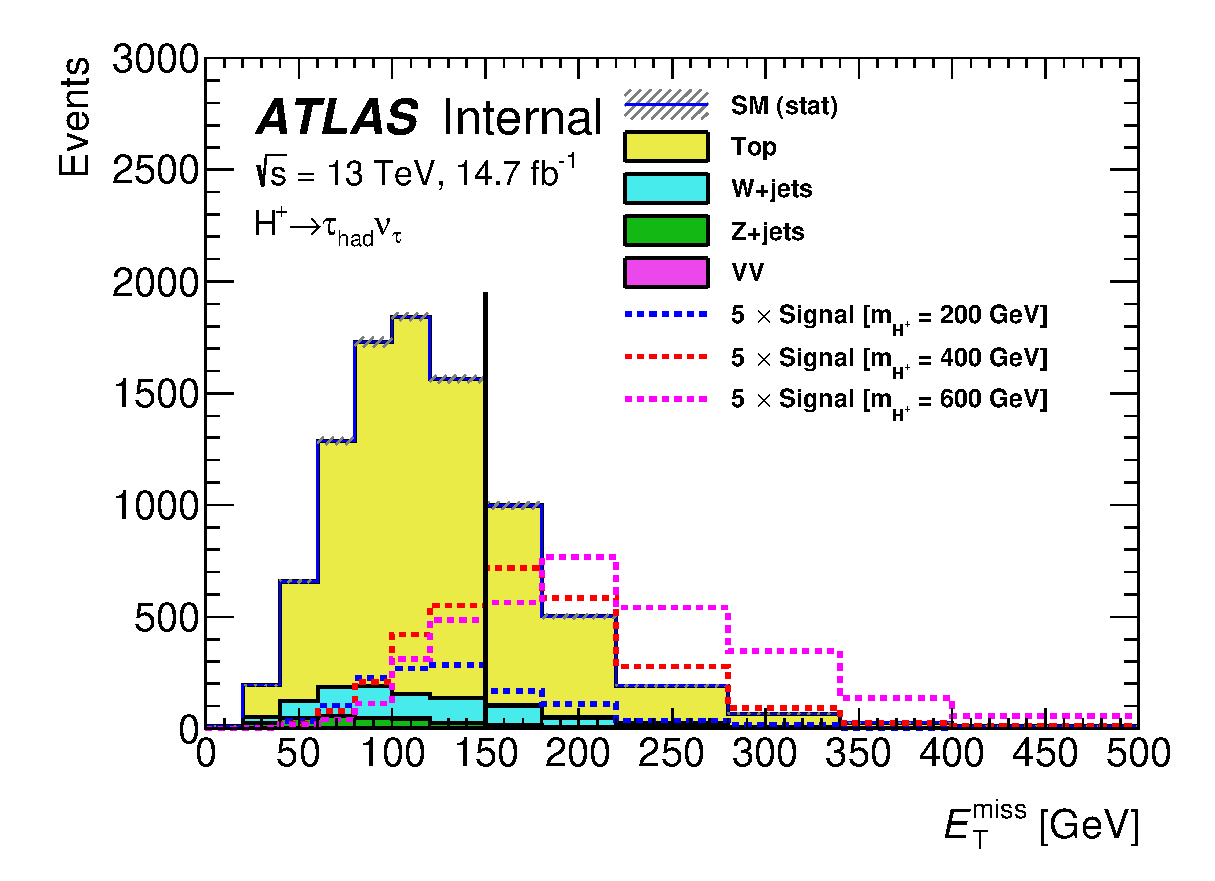
\includegraphics[width=\textwidth]{figures/met_nMinus1_expected.eps}
\caption{Expected \met\ distributions in the signal region, minus $\met>150$~\GeV}
\label{fig:preselectA}
\end{subfigure} % 
\begin{subfigure}{0.5\textwidth}
   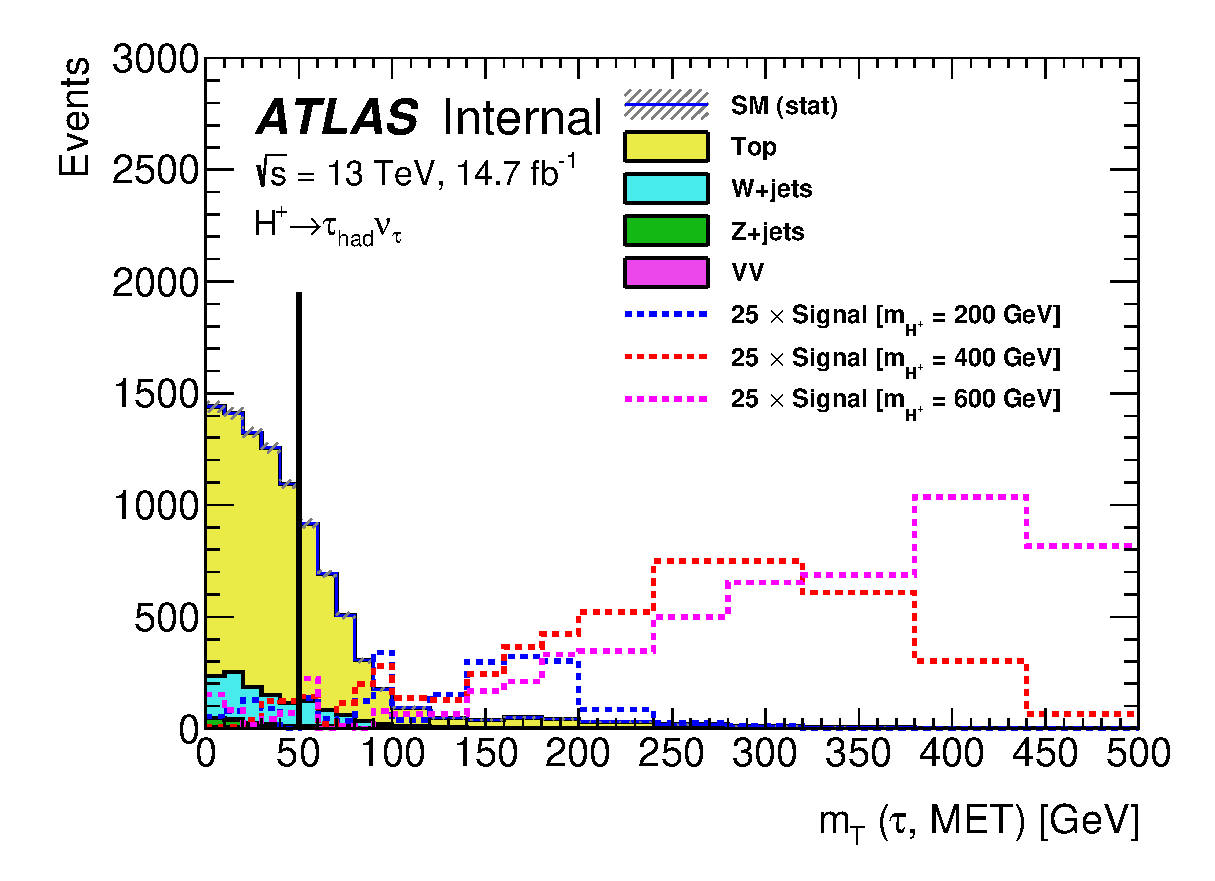
\includegraphics[width=\textwidth]{figures/mT_nMinus1_expected.eps}
\caption{Expected \mT\ distributions in the signal region, minus $\mT>50$~\GeV}
\label{fig:preselectB}
\end{subfigure}
\caption{N-1 distributions after the full selection criteria have been applied. The black 
vertical line marks the point at which the variable being plotted is cut on}
\end{figure}

Events in which \met\ is mismeasured and is aligned to the $\tau$ direction are suppressed by the \mT\ 
requirement. Moreover, events from which $\mT<50$~\GeV\ are likely to contain $\Wplus\to\tau\nu$ processes rather 
than signal. The \met\ requirement suppresses background from QCD multijets. 

%%%%%%%%%%%%%%%%%%%%%%%%%%%%%%%
%% TRIGGER EFFICIENCY STUDIES
%%%%%%%%%%%%%%%%%%%%%%%%%%%%%%%

\subsection{Trigger Efficiency}
\par Although trigger decisions in Monte Carlo simulation are sufficient to evaluate and compare trigger 
efficiencies as demonstrated by Figure~\ref{fig:trigComp}, they may not perfectly model trigger decisions 
in data. As shown in Table~\ref{tab:sigReg}, trigger decisions in simulation are essential in predicting background 
processes that contaminate the signal region. To account for this potential mis-modelling, 
efficiencies in simulation were corrected to those in data. The efficiencies from data 
were extracted from a dedicated control region and binned in \met. The trigger 
efficiency in data, in an \met\ bin was then defined as 

\begin{equation}
\epsilon = \frac{\text{control region selection} + \text{Trigger}}{\text{control region selection}}
\end{equation}  

where the `Trigger' is either \texttt{HLT\_xe70\_tc\_lcw} or \texttt{HLT\_xe90\_mht}. Both triggers require the 
event to pass an L1 trigger that demands at least 50 GeV in online \met. Apart from passing 
the clean-event selection, the control region selection is defined as follows :
\begin{enumerate}
\item exactly one loosely identified and loosely isolated electron, trigger matched to \\ \texttt{HLT\_e26\_lhtight\_iloose\_L1EM20VH};
\item exactly one loosely identified $\tauvis$ with at least 26~\GeV;
\item and at least two reconstructed jets, one of which must be $b-$tagged.
\end{enumerate} 

\par A similar control region with exactly one muon and no electrons was also considered. 
%Without loss of generality, efficiencies from the former region are chosen. 
\mT\ and \met\ distributions in the 1-electron control region are shown in 
Figure~\ref{fig:trigReg}. Here, contributions from processes in which jets are reconstructed as \tauvis ($j\to\tau$), or 
those in which non-$\tau$ leptons are reconstructed as \tauvis ($l\to\tau$), 
were estimated using methods described in Section~\ref{sec:bkgCh}. As will become clearer in 
the said section, application of those methods in this region requires some careful extrapolations 
that compensate for differences in topological structures in the two regions. Estimations shown 
in Figure~\ref{fig:trigReg} are rather ad-hoc because they do not take into account these differences.  
Consequently, there is an obvious mis-modelling of physics processes in the low 
\met\ and \mT\ regions, as shown by the disagreement between data and simulation.
Reasonable agreement between data and predictions is observed at $\met>50$~\GeV.
Since trigger thresholds 
studied were at minimum $\met=70$, disagreements in the low \met\ and low \mT\ regions did not have significant impact on 
measurements.

\begin{figure}[!h]
\begin{subfigure}{0.5\textwidth}
   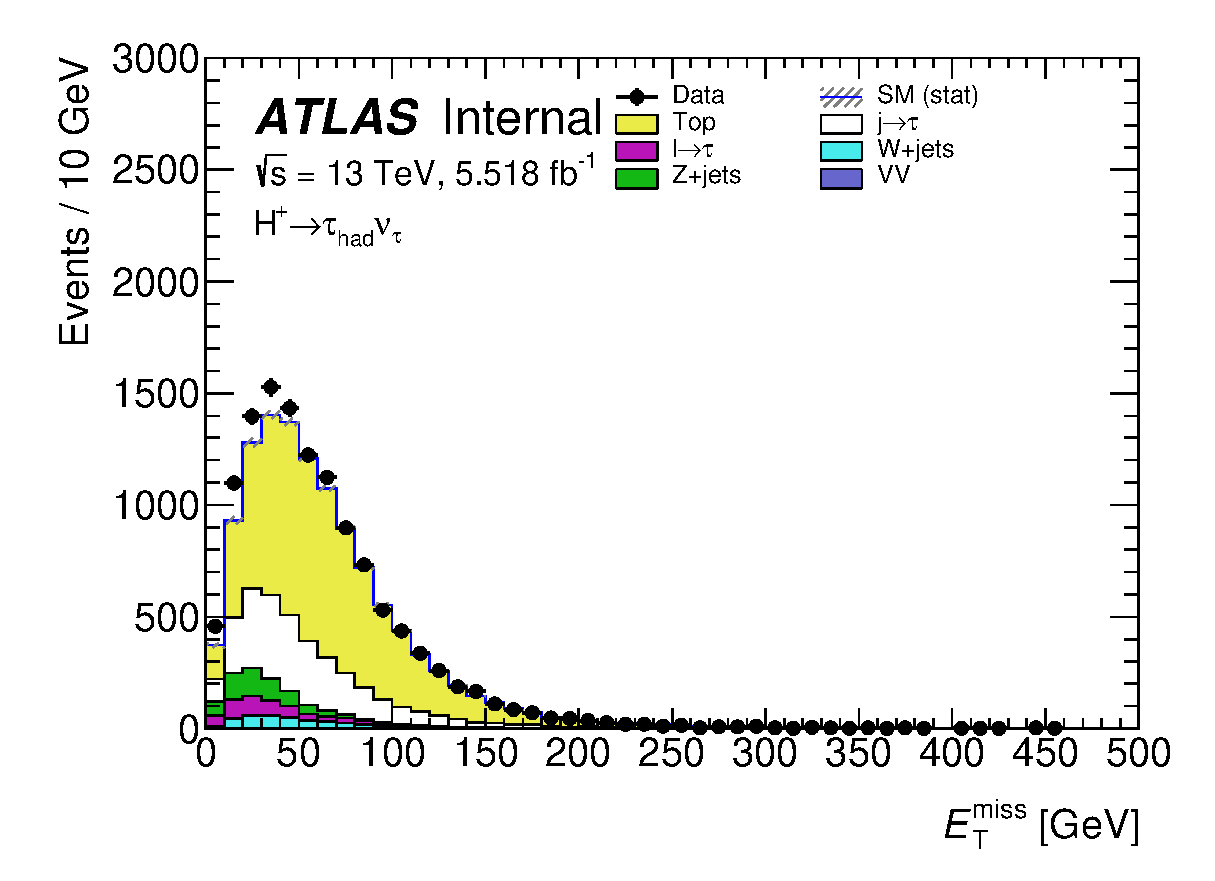
\includegraphics[width=\textwidth]{figures/all_CutNoMatchNbjets_met_lin_forTriggers.eps}
\end{subfigure} % 
\begin{subfigure}{0.5\textwidth}
   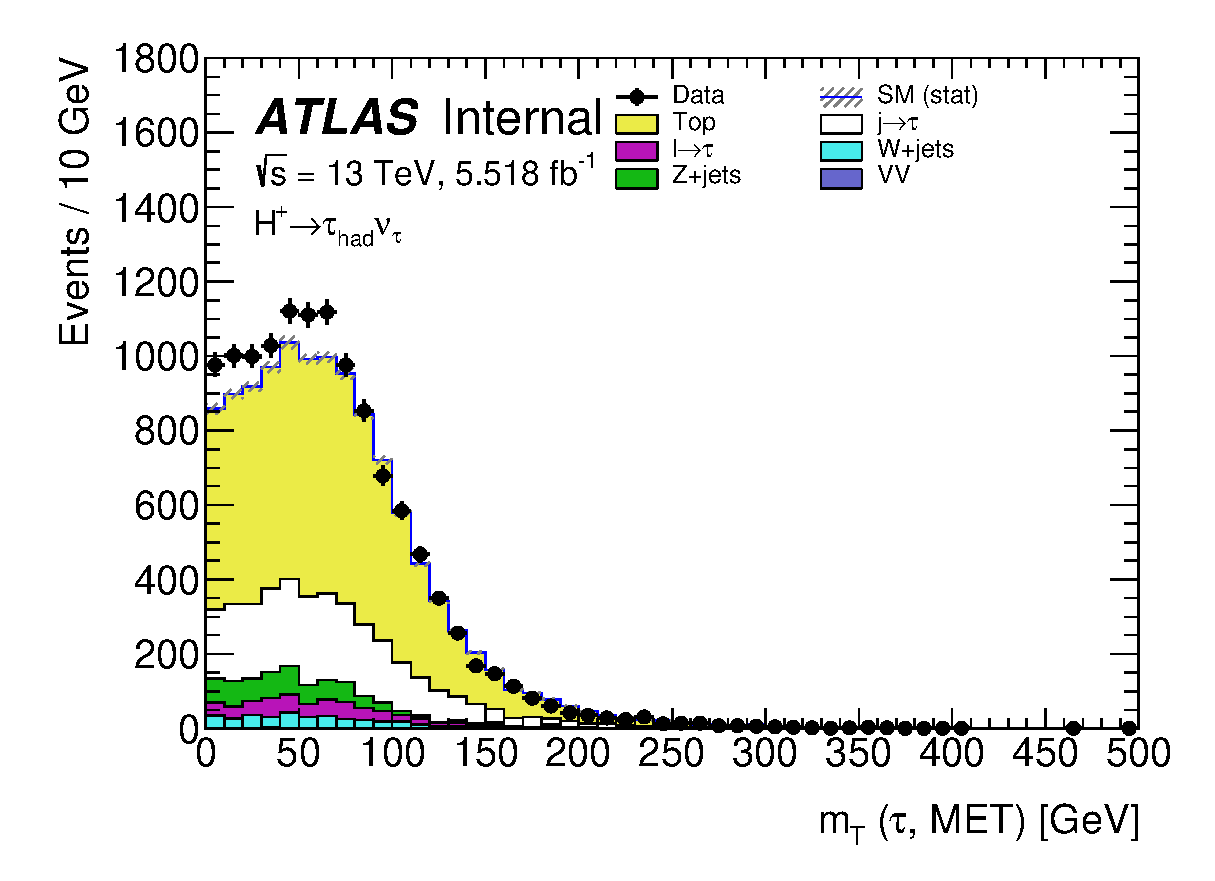
\includegraphics[width=\textwidth]{figures/all_CutNoMatchNbjets_mT_lin_forTriggers.eps}
\end{subfigure}
\caption{\met\ and \mT\ distributions in the control region used to measure trigger efficiencies. Since trigger thresholds 
studied were at minimum $\met=70$, disagreements in the low \met\ and low \mT\ regions did not have significant impact on 
measurements}
\label{fig:trigReg}
\end{figure}

\par To obtain continuous efficiency distributions, the binned efficiencies from data were
 fitted to the error function, parametrized as 

\begin{equation}
F(x) = p_0.\left [ 1 + \text{erf}\left ( \frac{x-p_1}{p_2}\right )\right ] + p_3
\end{equation}

where initial values for the $p_i$ were repeatedly changed until an optimal 
fit was obtained. The optimization of the fit was quantified by the $\chi^2$ distribution. 
This procedure was done separately for the 2015 and 2016 datasets. The efficiency 
distributions and their respective fits are shown in Figures~\ref{fig:trigFitA} and~\ref{fig:trigFitB}, 
reaching 100\% efficiency at about \met$=$250~\GeV. In these plots the region from which most of the 
events in the signal region lie, $150<\met<250~\GeV$, is marked with vertical dashed lines.  
 
\begin{figure}[!h]
\begin{subfigure}{0.5\textwidth}
   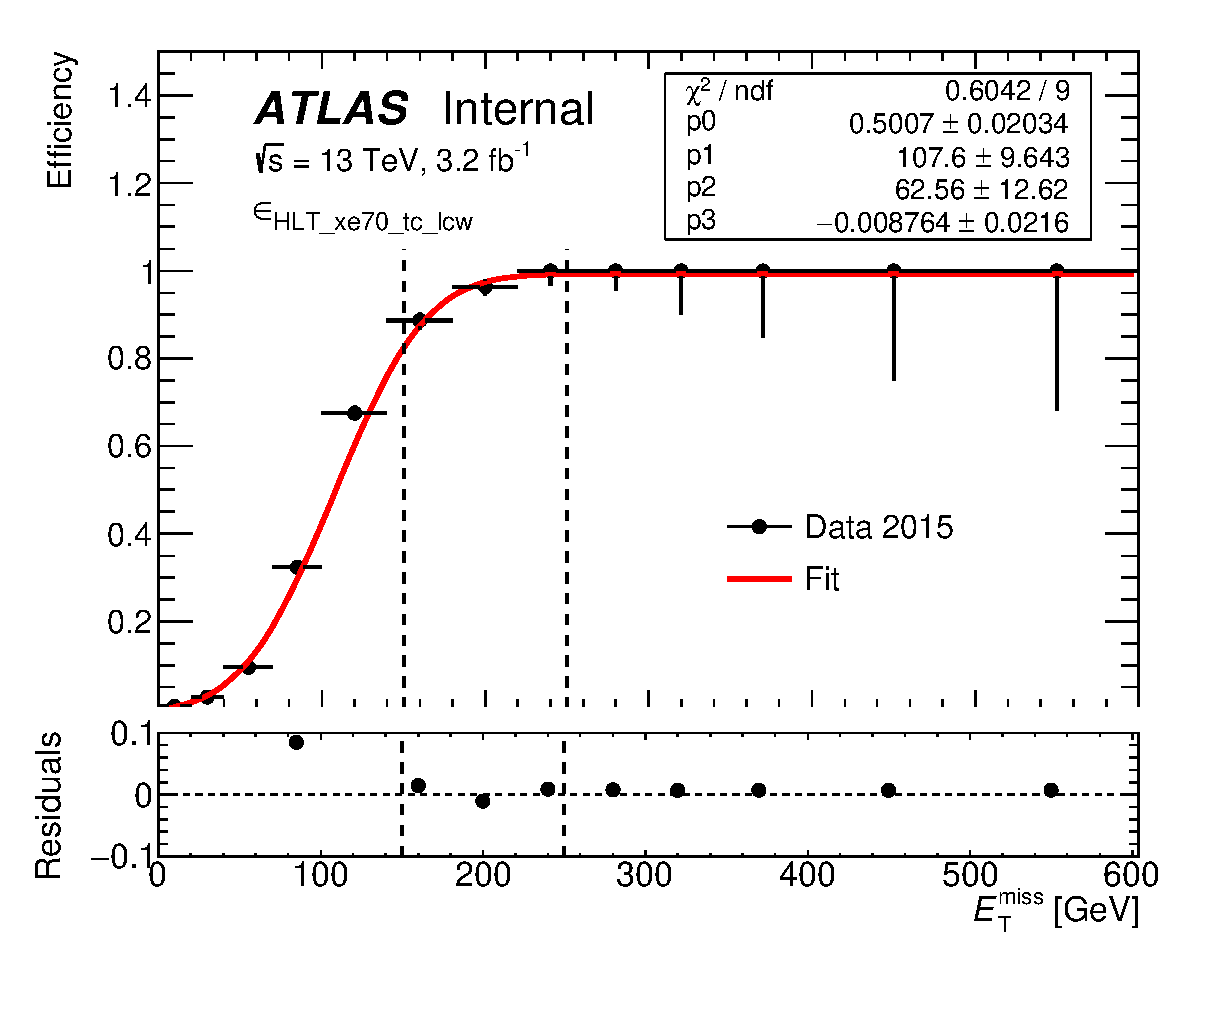
\includegraphics[width=\textwidth]{figures/xe70_tclcw_data15_fitted.eps}
\caption{2015 data-set}
\label{fig:trigFitA}
\end{subfigure} % 
\begin{subfigure}{0.5\textwidth}
   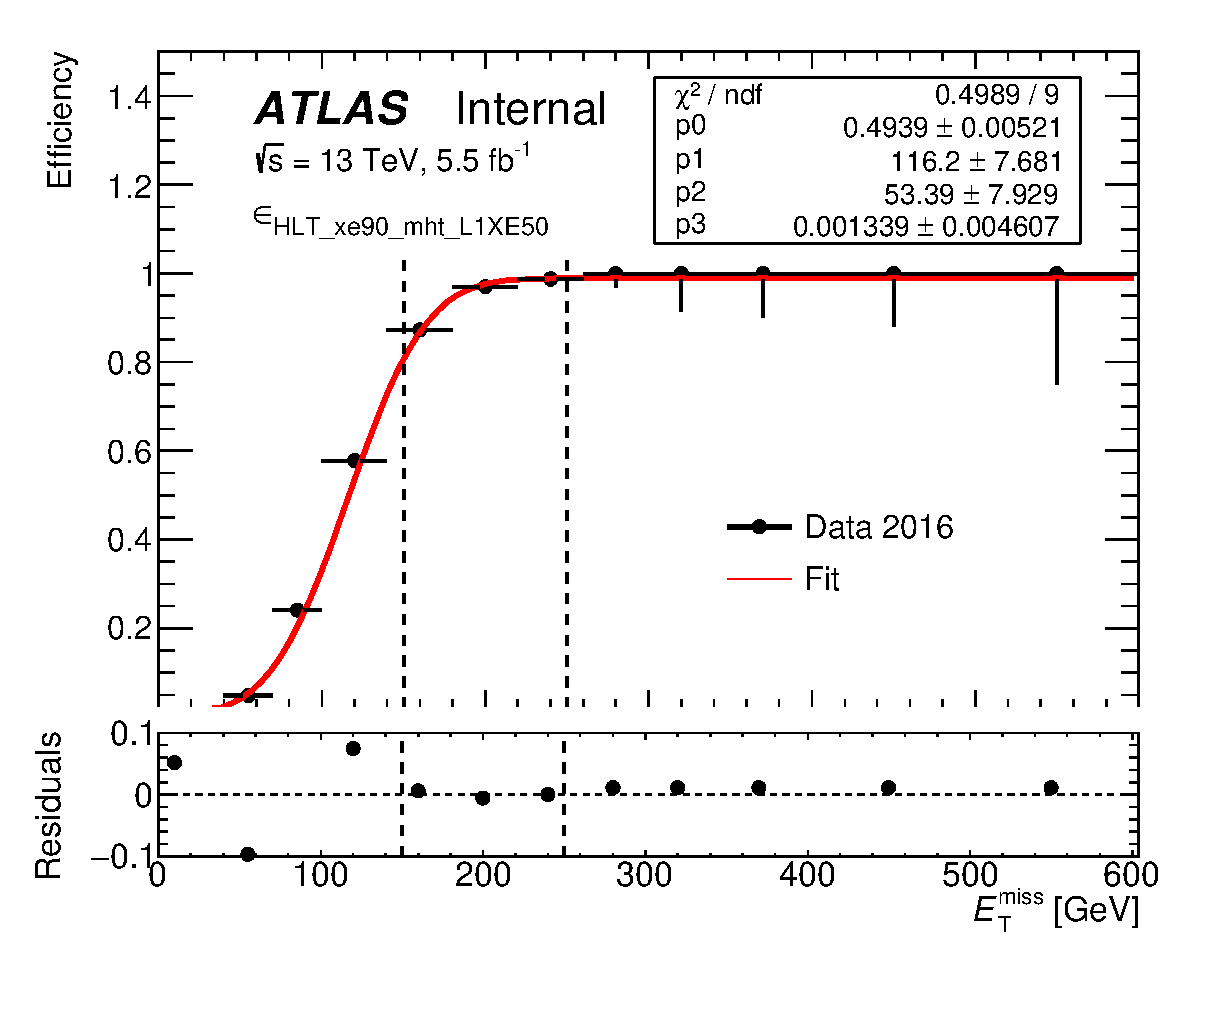
\includegraphics[width=\textwidth]{figures/xe90_mht_data16_fitted.eps}
\caption{2016 data-set}
\label{fig:trigFitB}
\end{subfigure}
\caption{Plots showing trigger efficiency fits}
\end{figure}


\section{Background Modelling}
\label{sec:bkgCh}
\par Backgrounds are categorized into 3 classes that are defined according to the 
source of the $\tauvis$.   
If the \tauvis\ is reconstructed from a $\tau$ lepton, it is referred to as a {\it true} 
$\tauvis$. Treatment of this category has been briefly discussed in Section~\ref{sec:evSelCh} and 
is discussed in more detail in Section~\ref{sec:truetau}. Events in which a $\tauvis$ is reconstructed from an electron or muon  
constitute the $l\to\tau$ background. More on this in Section~\ref{sec:lepToTau}.
Events in which a $\tauvis$ is reconstructed from a jet, be it from a quark or gluon, 
constitute the $j\to\tau$ background. More on this in Section~\ref{sec:jetToTau}. 
The $j\to\tau$ and $l\to\tau$ backgrounds are collectively 
referred to here as the {\it Mis-ID}\footnote{For `misidentified $\tau$'.}  backgrounds. 

\subsection{Lepton to $\tau$}
\label{sec:lepToTau}
\par For the $l\to\tauvis$ backgrounds only the $e\to\tauvis$ contribution is estimated; 
the $\mu\to\tauvis$ background contamination in the signal region was found to be an order of magnitude smaller. 
Backgrounds in which a $\tauvis$ is matched in $\Delta R$ to an electron are 
applied a scale factor, which encodes the probability of an electron to fake a $\tauvis$. This 
scale factor is dependent on whether the reconstructed $\tauvis$ is 1-prong or 3-prong, so separate 
computations are performed. This scale factor was also observed to be dependent on $\eta$, so it was 
parametrized accordingly. 

\par To measure these scale factors the following $\Zee$ control region is designed 

\begin{enumerate}
\item exactly one electron matched to a single electron trigger;
\item exactly one medium \tauvis\ with charge opposite to the electron;
\item no $b-$tagged jets; and 
\item $\mT(e,\met)<40$~\GeV
\end{enumerate}  

Here, the electron is used as a tag, and the \tauvis\ as a probe. 
To ensure that the \tauvis\ and the electron originate from the \Zboson, the mass of the 
$e-\tauvis$ system is restricted to between 80~\GeV\ and 100~\GeV.

\par The scale factors were computed as the ratio of events that pass all selection criteria to those 
that pass all but not necessarily the presence of the \tauvis. This computation was 
performed in both data and simulation. In data, non-\Zee\ events were subtracted from data 
before the calculation was performed. Figure~\ref{fig:lepToTau} shows these scale factors, 
parametrized in $\eta$. They range from 0.5\% to 2.5\%.    

\begin{figure}[h]
\centering
   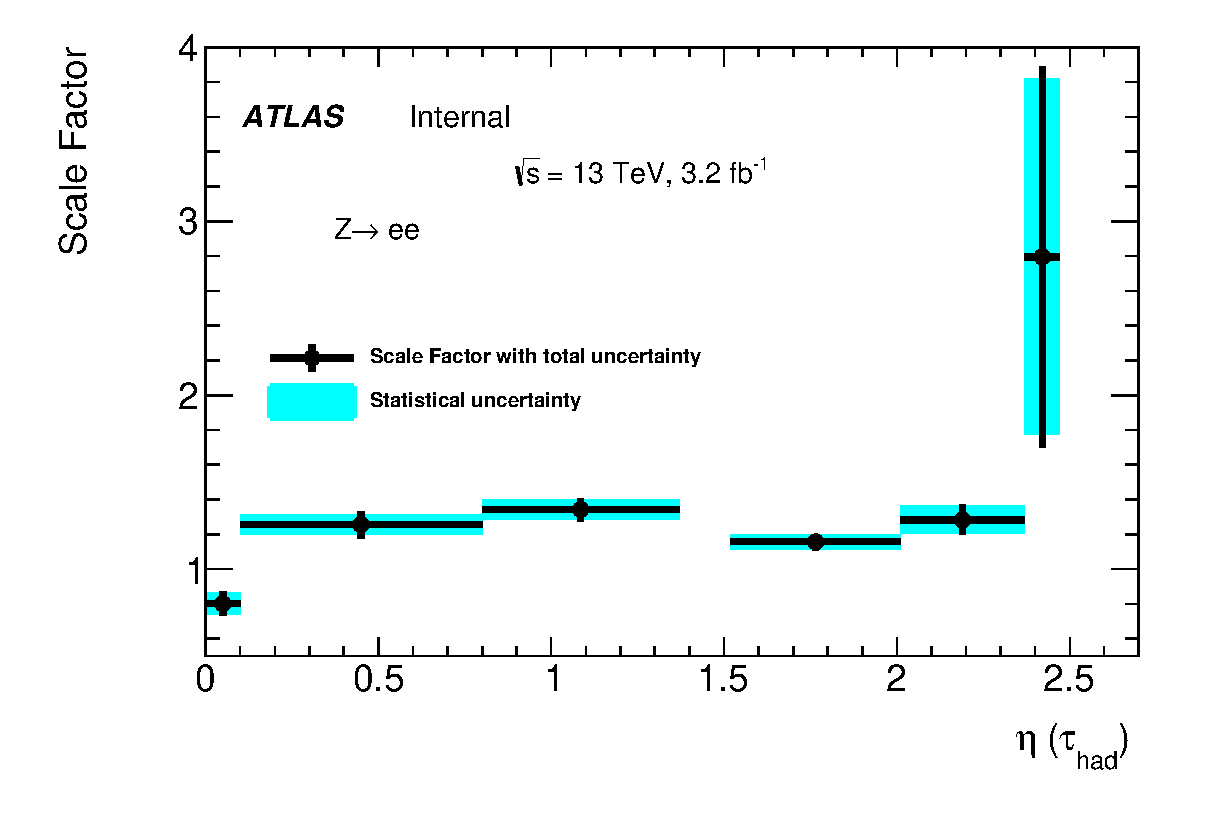
\includegraphics[width=0.8\textwidth]{figures/c7_evto_SF.eps}
\caption{Plot showing the probability of an electron to fake a \tauvis, parametrized in $\eta$}
\label{fig:lepToTau}
\end{figure}
 
\subsection{$j\to\tau$ backgrounds}
\label{sec:jetToTau}
\par The {\it Fake Factor Method (FFM)}, described in this section, is used to estimate $j\to\tau$ backgrounds. 
The strategy is to extrapolate to the signal region the number of events where a $\tauvis$ is reconstructed from a quark 
or gluon initiated jet, from a control region rich with quark or gluon initiated jets.
The extrapolation is handled by scale factors, referred to as {\it Fake Factors (\FF)}. 
During this extrapolation large uncertainties are accrued from differences between the said control region and 
the signal region. To minimize them, the control region is designed to be as close to the 
signal region as possible. The control region used here, referred to as 
the {\it anti-$\tau$} region, only differs from the signal region in that the reconstructed  
 \tauvis\ fails the identification criteria required in the signal region.  
More specifically, the anti-$\tau$ region is identical to the signal region except that its \tauvis\ is required 
to be not loose and its jet BDT score is required to be greater than 0.5.
Events in which a quark or gluon initiated jet fakes a $\tau$ lepton in the signal region, $N^\tau_{\text{fakes}}$.
are therefore estimated by weighting events in the anti-$\tau$ region, $N^{\text{anti-}\tau}_{\text{fakes}}$,
 with $\FF$ as summarized in Equation~\ref{eq:ffDef}. 

\begin{equation}
N^\tau_{\text{fakes}} = N^{\text{anti-}\tau}_{\text{fakes}}\times\FF
\label{eq:ffDef}
\end{equation}

\par The $\FF$ are measured from a region in data that is rich in quark or gluon initiated jets. This {\it 
measurement} control region must be different from the control region in which the $\FF$ are applied (e.g the 
one described in the preceding paragraph). It is however similar in the sense that the \tauvis\ is required 
to pass the same identification criteria. In this case it is required to be not loose and have 
a jet BDT score greater than 0.5. In that respect, it is referred to as the {\it anti-$\tau$-id}\footnote{To 
emphasize, this is not to be confused with the anti-$\tau$ region in which the \FF\ are applied.} region. 
A similar control region, but with the \tauvis\ required to pass the identification criteria that is 
demanded in the signal region, is also defined. This is called the $\tau-id$ control region.  
The number of events in the anti-$\tau$-id control region, $N_{\text{anti-}\tau\text{-id}}$, 
and the number of events in the $\tau-$id region, 
$N_{\tau-\text{id}}$, are extracted. The fake factors are then computed as 

\begin{equation}
\FF = \frac{N_{\tau-\text{id}}}{N_{\text{anti-}\tau\text{-id}}} 
\end{equation}

\subsubsection{Pre-validation}
\par To test the effectiveness of this method, fake factors from \ttbar\ simulation are applied 
on \ttbar\ events after a different selection criteria has been applied. 
Simulated \ttbar\ events with exactly one not loose $\tauvis$ make up the anti-$\tau$-id 
region. Similarly, events with exactly one medium $\tauvis$ make up the $\tau-$id region.
Since the probability of a jet being mis-identified as a $\tauvis$ depends on the jet substructure, \FF\ 
are parameterized in terms of parameters that describe the jet substructure. These are 
\begin{enumerate}
\item Transverse momentum of the \tauvis, $\pt^\tau$. This parameter is sensitive to the 
gluon or quark fractions in the jet;
\item $\tau$ decay mode. This is essentially a measure of the number of pions that the $\tau$ 
lepton decays to; and 
\item $b-$tagger weight. 
\end{enumerate}    

The \FF\ obtained in the \ttbar\ MC simulation are applied to \ttbar\ events that pass the 
preselection criteria defined in Table~\ref{tab:sigReg}. Figure~\ref{fig:ttClo} shows comparisons 
between estimation using \FF\ and direct MC estimation. 

\begin{figure}[h]
\begin{subfigure}{0.5\textwidth}
   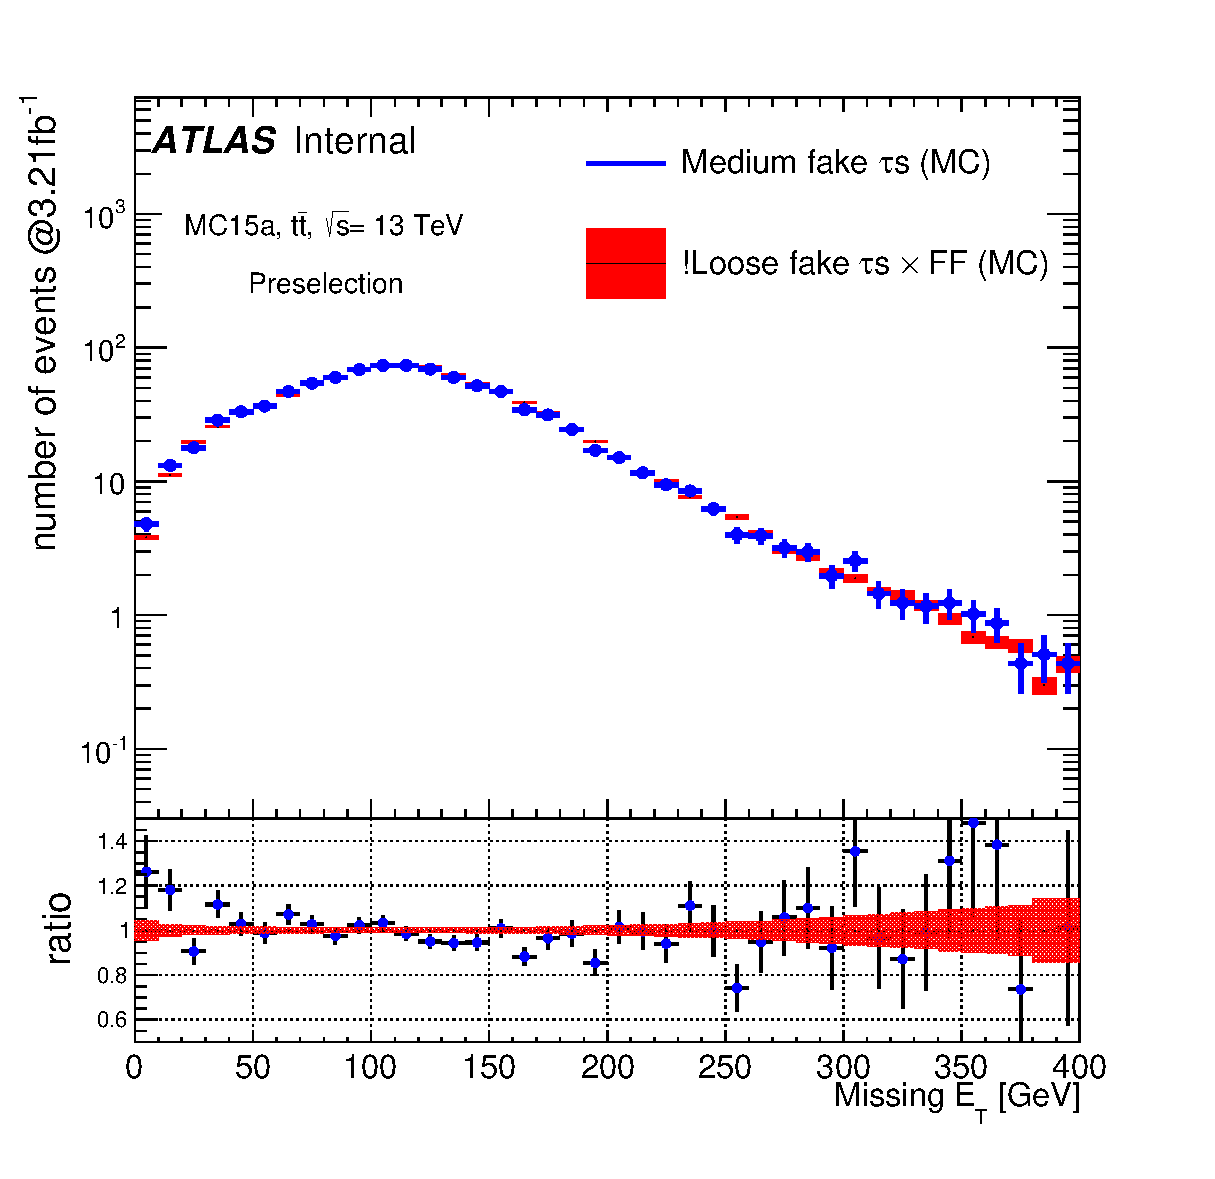
\includegraphics[width=\textwidth]{figures/Fake_MMClosure_met.eps}
\caption{\met\ in \ttbar closure region}
\end{subfigure} % 
\begin{subfigure}{0.5\textwidth}
   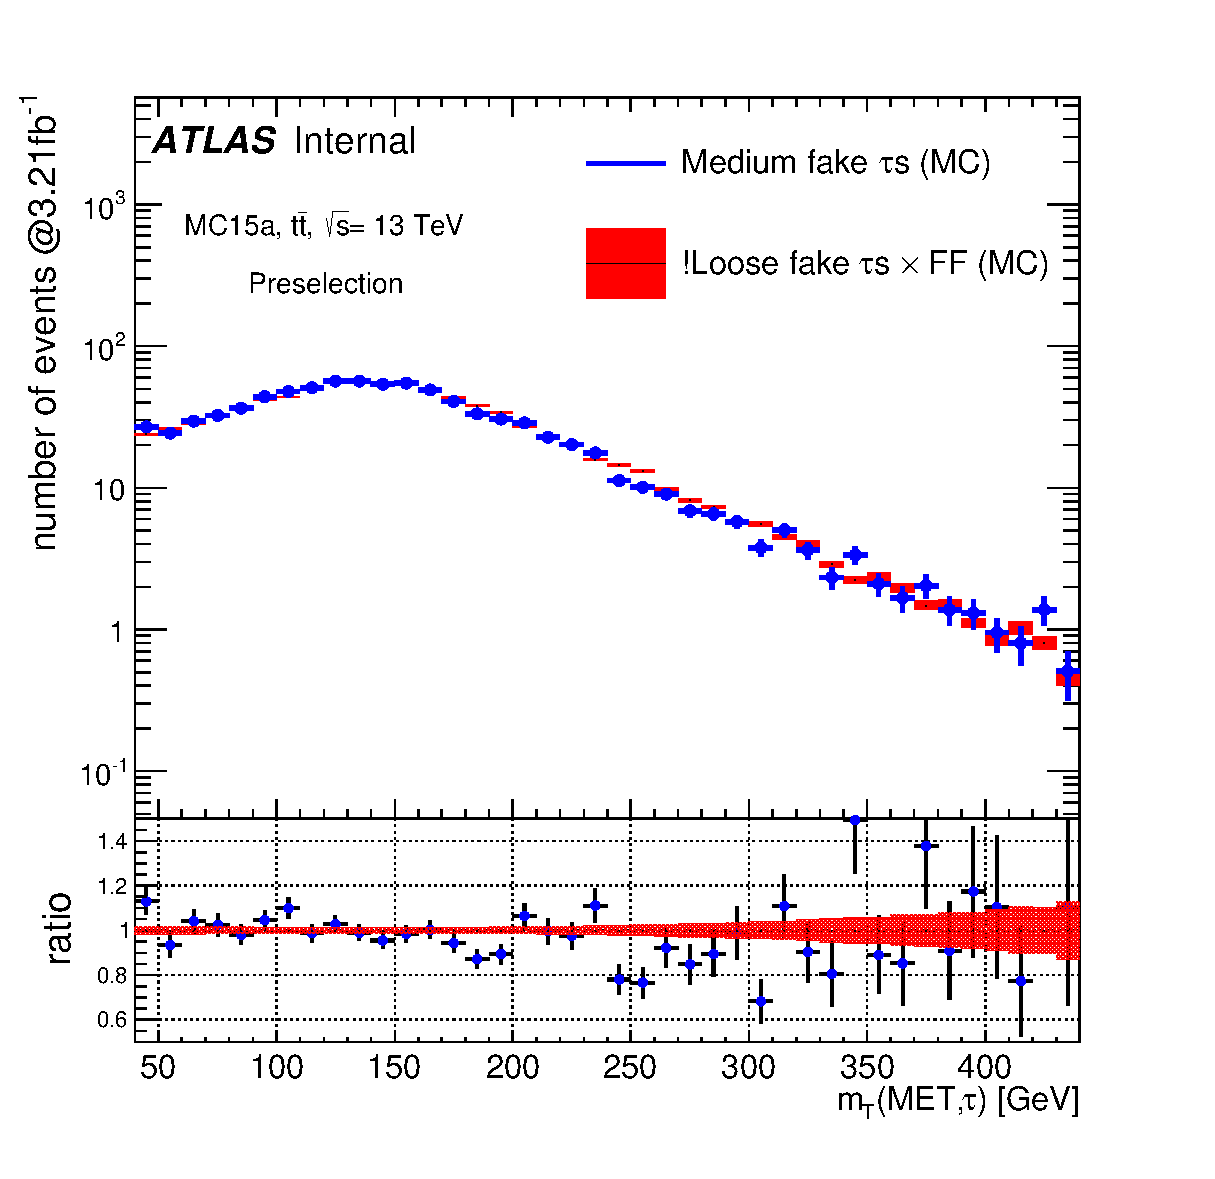
\includegraphics[width=\textwidth]{figures/Fake_MMClosure_MT.eps}
\caption{\mT\ in \ttbar closure region}
\end{subfigure}
\caption{Plots showing the comparison of estimations using direct MC versus the \FF\ method}
\label{fig:ttClo}
\end{figure}

\subsubsection{\FF\ measurement control regions}
\par Two regions in data that are rich in jets reconstructed as \tauvis\ are 
used to extract \FF. One of these regions is designed to be dominated by QCD multi-jet events,
 while the other is dominated by $\Wjets$ events. The former will be referred to as the {\it multi-jet} 
region while the latter as the $\Wjets$ region. The fraction of jets that are initiated by quarks 
in the multi-jet region is roughly the same as the fraction of jets that are initiated by gluons 
in the same region. In contrast, the \Wjets\ region is dominated by jets initiated by light-flavor quarks.
Since the substructure of jets is expected to depend on their source, it is necessary to evaluate the impact 
of these different sources on the final results. The multi-jet region is used as the nominal region for measuring 
\FF. Measurements taken from \Wjets\ are used as a systematic variation corresponding to the inclusion of a higher 
fraction of light-flavor quarks.  

\par The multi-jet region is similar to the signal region. It differs from the signal region 
in that it requires 0 $b-$tagged jets and $\met<80$~\GeV. Figure~\ref{fig:multiCR} shows 
\mT\ distributions for processes that pass this selection criteria. The \Wjets\ region is more different to the signal region than 
the multi-jet region. \met\ is required to be at most 150~\GeV, exactly one electron or muon must 
be present, no $b-$tagged jets, and $\mT(e/\mu,\met)>60$~\GeV. Figure~\ref{fig:wjetsFFcr} shows 
\mT\ distributions in this region.  

\begin{figure}[!h]
\begin{subfigure}{0.5\textwidth}
   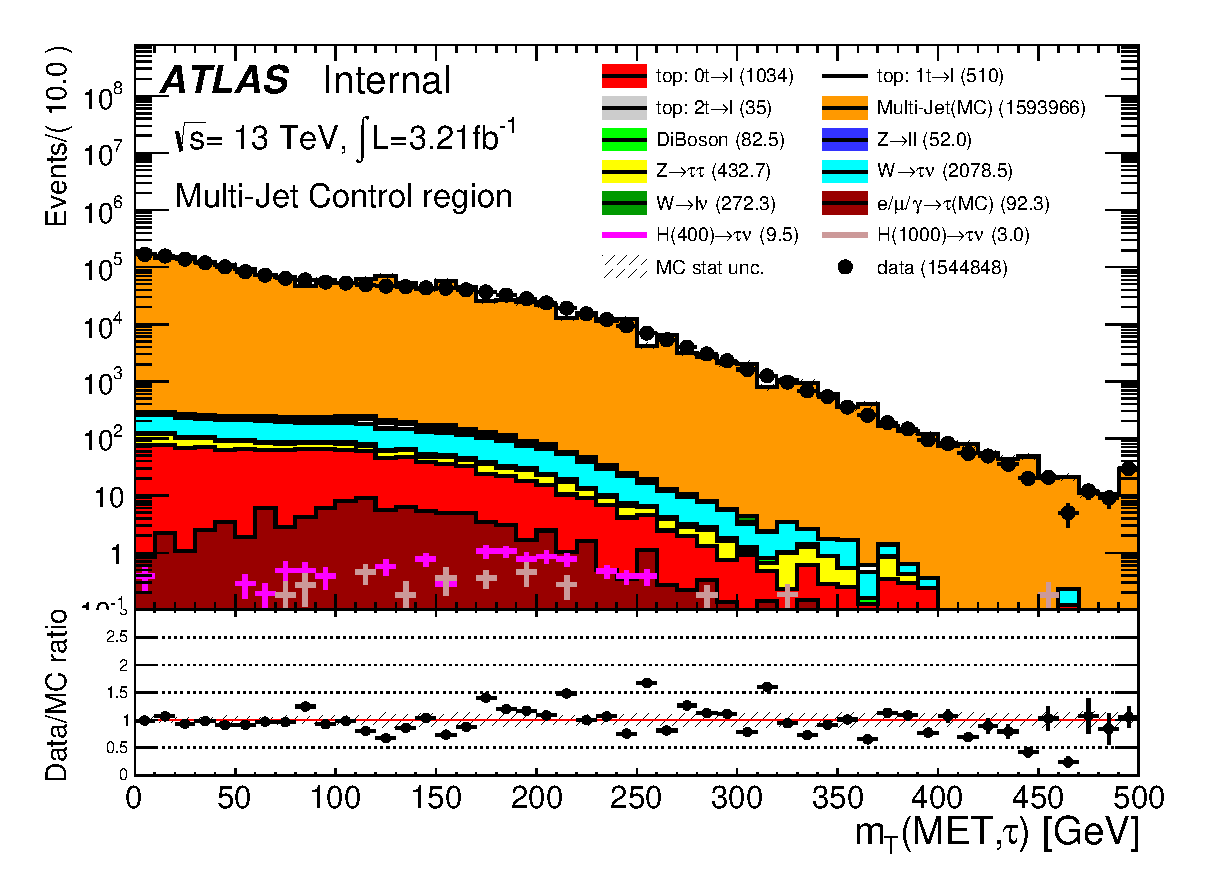
\includegraphics[width=\textwidth]{figures/data15_QCD_MT_log.eps}
\caption{Multi-jet region for \FF}
\label{fig:multiCR}
\end{subfigure} % 
\begin{subfigure}{0.5\textwidth}
   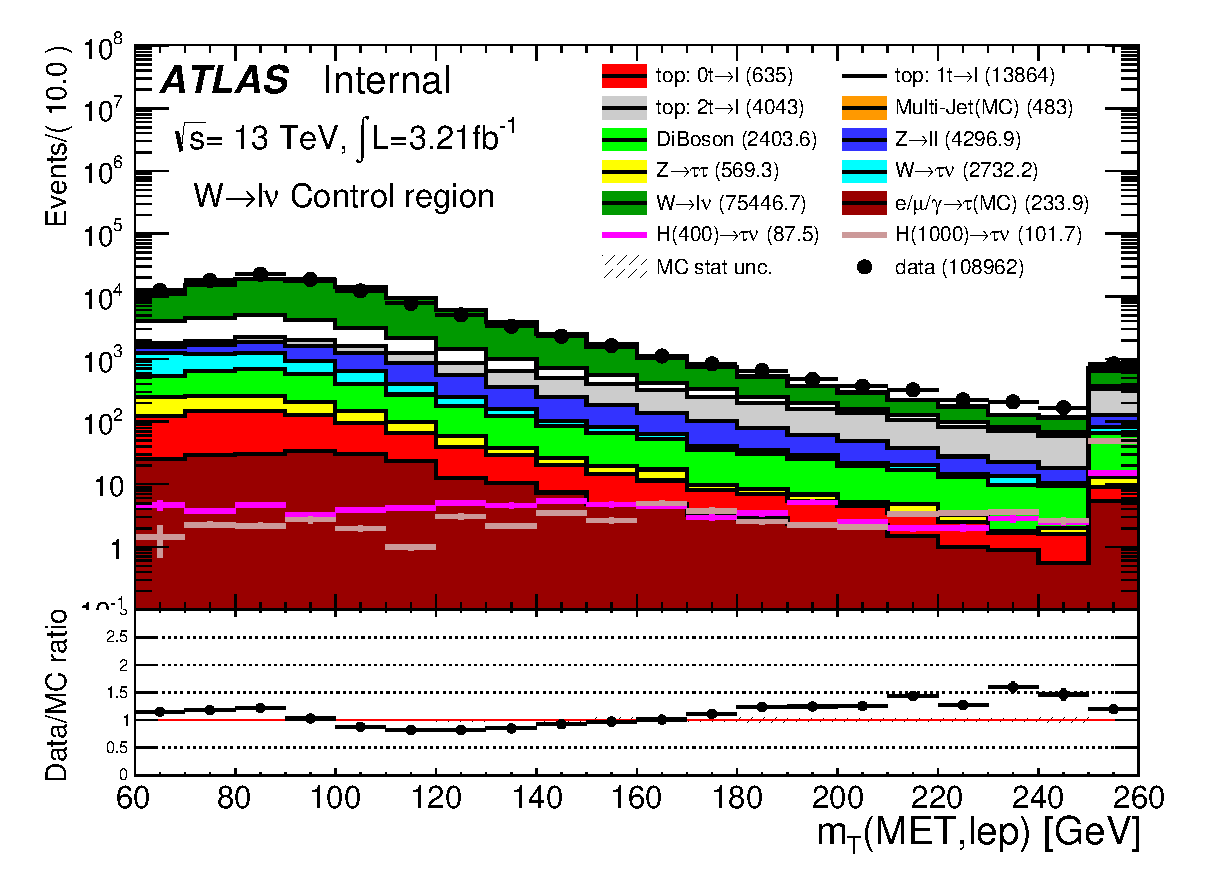
\includegraphics[width=\textwidth]{figures/data15_WCR_WlepMT_log.eps}
\caption{\Wjets\ region for \FF}
\label{fig:wjetsFFcr}
\end{subfigure}
\caption{Plots showing \mT\ distributions in the multi-jet and the \Wjets\ control regions}
\end{figure}

\par Figures~\ref{fig:ffA} and \ref{fig:ffB} show the \FF\ obtained from the multi-jet region. 
They are parametrized in $\pt$ computed separately for 1-prong and 3-prong $\tauvis$ candidates. 
Figure~\ref{fig:ffA} is from 2015 data while Figure~\ref{fig:ffB} is from 2016 data. The binning in 
\pt\ was optimized to have a minimal statistical uncertainty in each bin. For 2016 data the \FF\ dependence 
on the $b-$tag weight was insignificant so it wasnt pursued further.   

\begin{figure}[!h]
\begin{subfigure}{0.5\textwidth}
   \includegraphics[width=\textwidth]{figures/GetTauFFmed2D_2015.eps}
\caption{}
\label{fig:ffA}
\end{subfigure} % 
\begin{subfigure}{0.5\textwidth}
   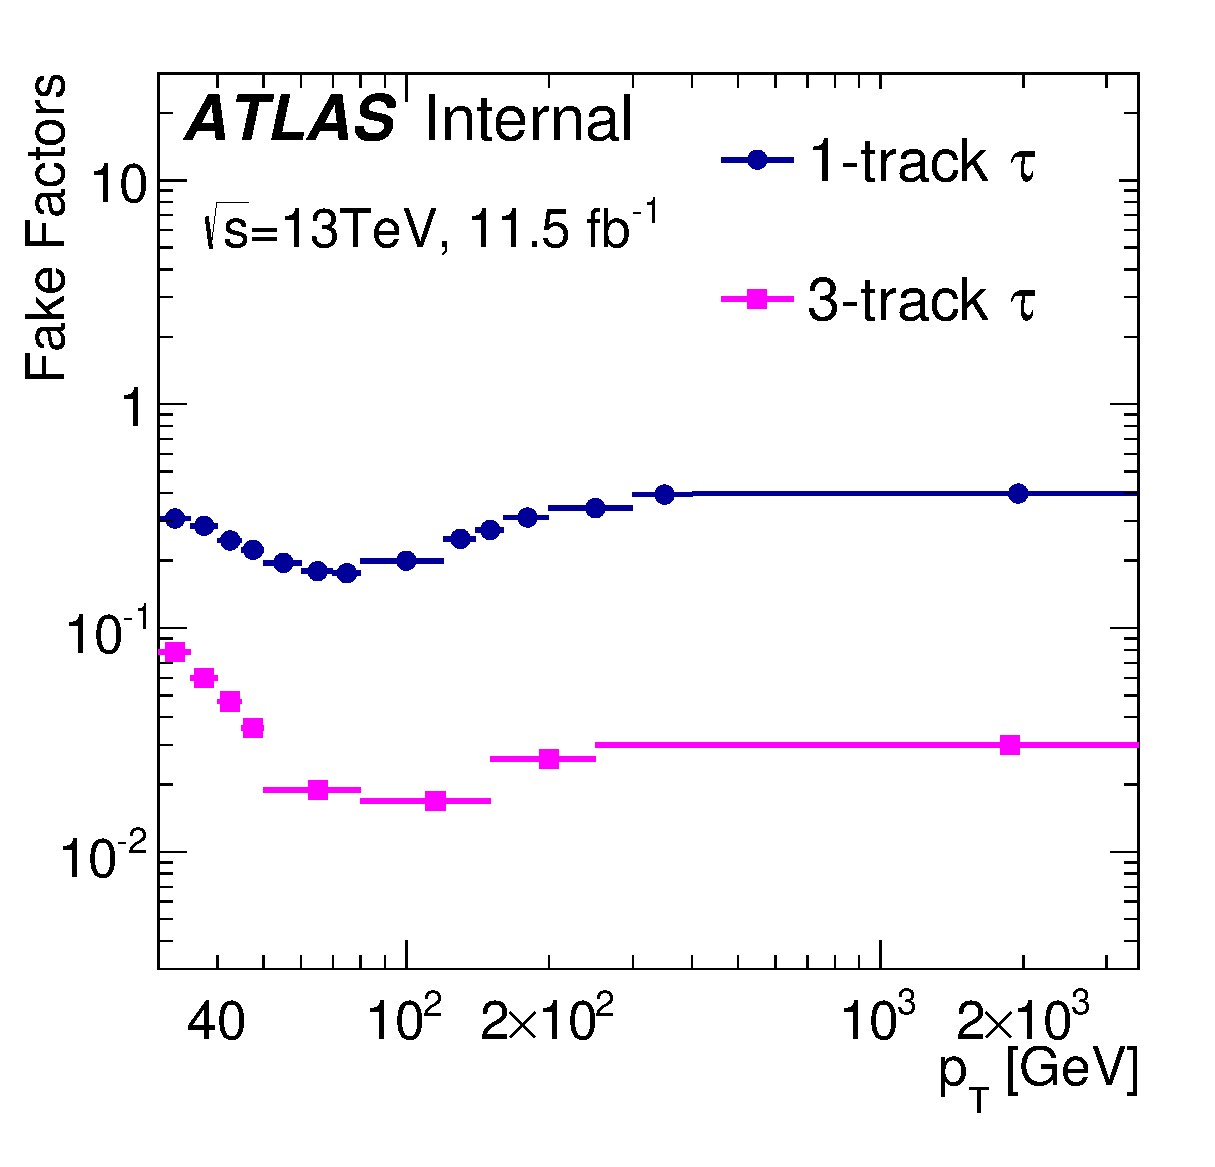
\includegraphics[width=\textwidth]{figures/GetTauFFmed2D_2016.eps}
\caption{}
\label{fig:ffB}
\end{subfigure}
\caption{Plots showing the measured \FF\ parametrized in \tauvis\ \pt}
\label{fig:ff}
\end{figure}

\subsubsection{Validation}
\par The \FF\ shown in Figure~\ref{fig:ff} were validated in several control regions. First is the 
multi-jet control region from which these \FF\ were measured. Figure~\ref{fig:clMultiJ} shows the 
estimated $j\to\tau$ contribution in this region, using the FFM. Overall, the estimation shows good 
\FF\ modelling in this region. 

\begin{figure}[h]
\begin{subfigure}{0.5\textwidth}
   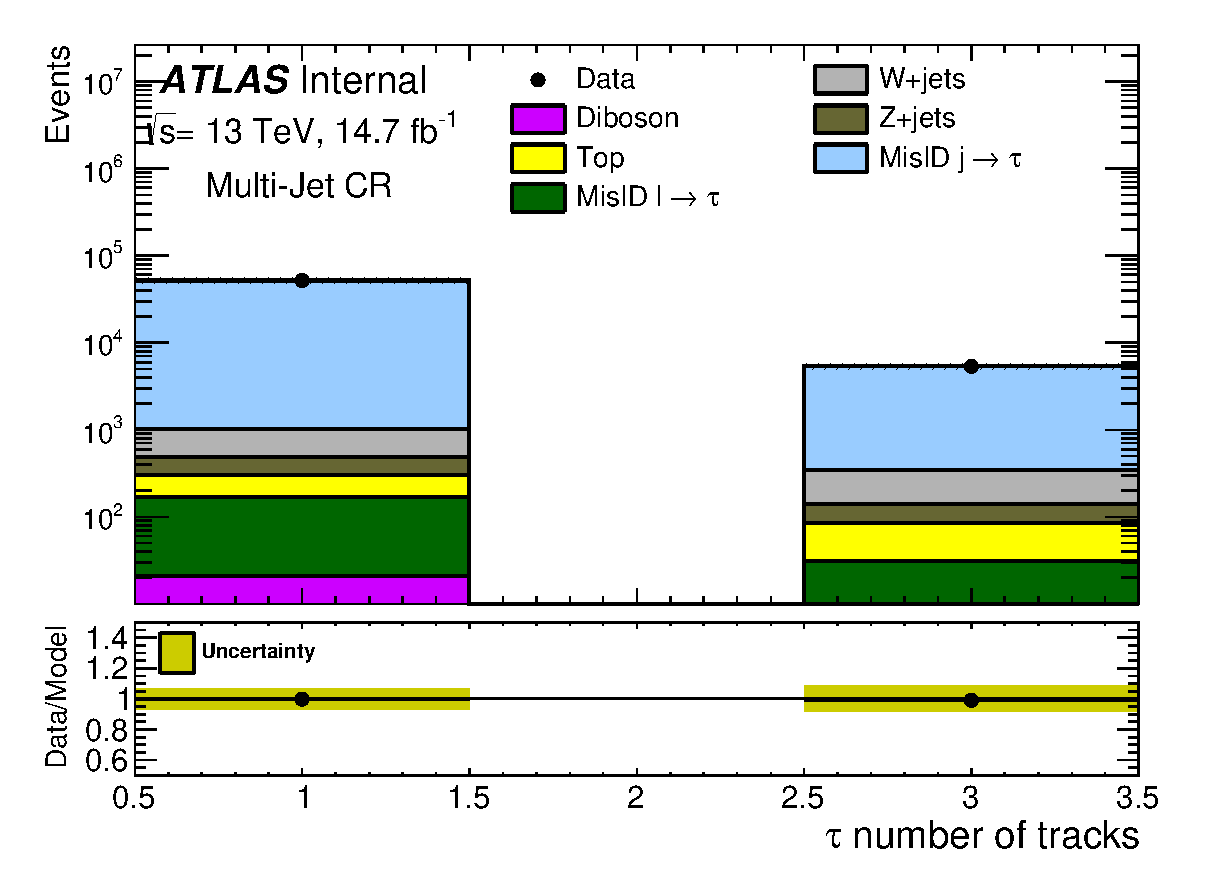
\includegraphics[width=\textwidth]{figures/DDQCD15_QCD_nTrack.eps}
\caption{}
\end{subfigure} % 
\begin{subfigure}{0.5\textwidth}
   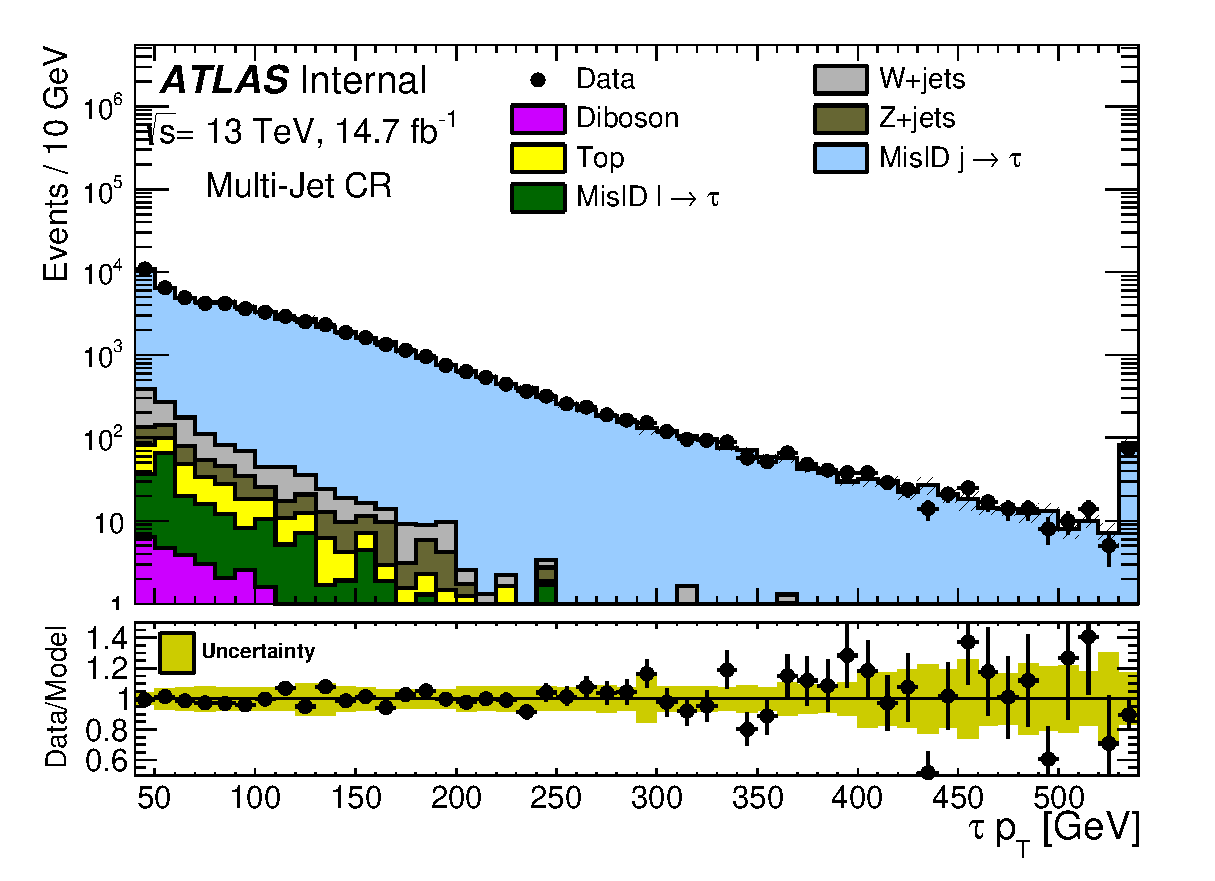
\includegraphics[width=\textwidth]{figures/DDQCD15_QCD_taupt_log.eps}
\caption{}
\end{subfigure}
\begin{subfigure}{0.5\textwidth}
   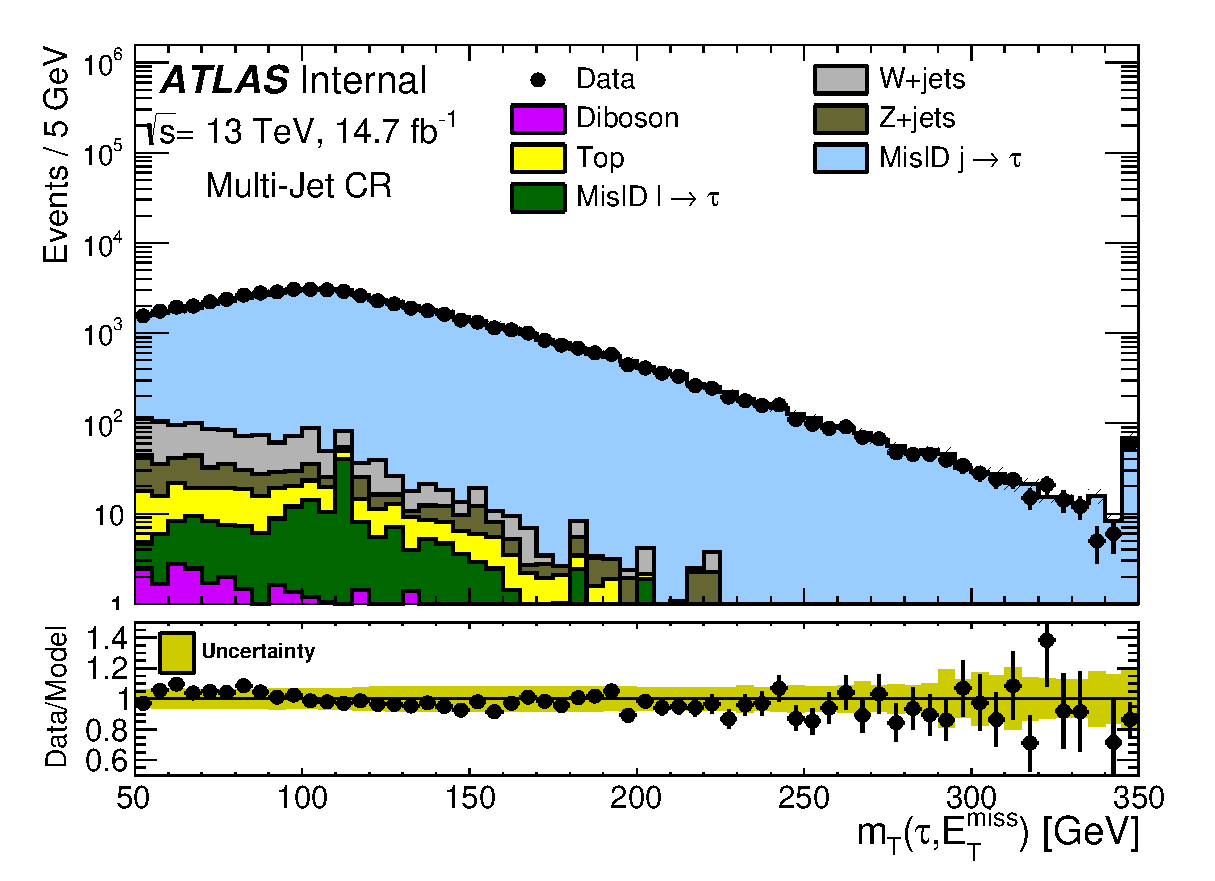
\includegraphics[width=\textwidth]{figures/DDQCD15_QCD_MT.eps}
\caption{}
\end{subfigure} % 
\begin{subfigure}{0.5\textwidth}
   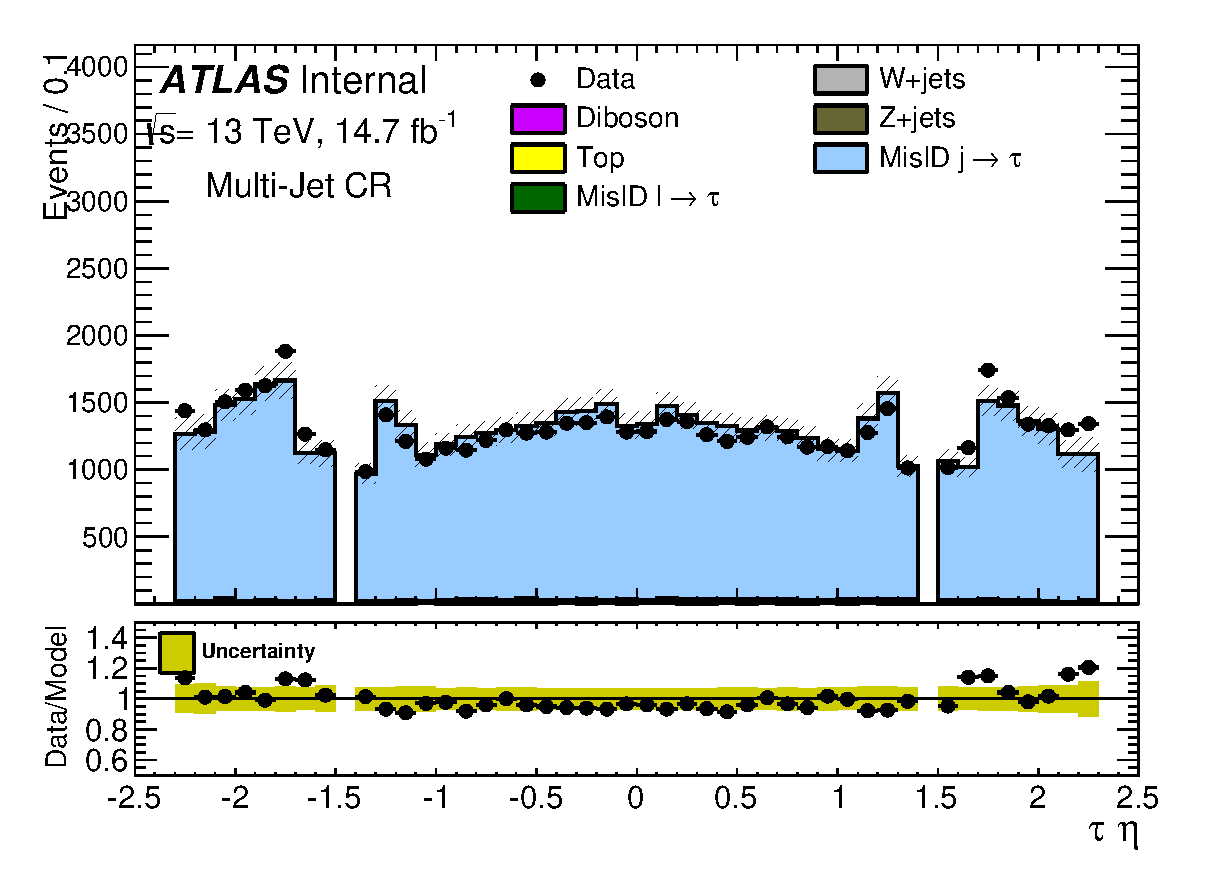
\includegraphics[width=\textwidth]{figures/DDQCD15_QCD_taueta.eps}
\caption{}
\end{subfigure}
\caption{\FF\ closure plots in the multi-jet measurement control region}
\label{fig:clMultiJ}
\end{figure}

\par To evaluate the \FF\ robustness to change in jet composition, two 
control regions were used. As alreadly mentioned, the \Wjets\ region is dominated by jets initiated 
by light-flavored quarks. Contrastingly, a region rich in \ttbar\ events is dominated by 
jets initiated by heavy-flavored quarks. These two regions were used to evaluate the impact of 
heavy versus light-flavored quarks on \FF\ modelling, and vice-versa. Figure~\ref{fig:clWjets} and Figure~\ref{fig:clTTBar}
show the estimated $j\to\tau$ background using the \FF\ method  in the $\Wjets$ and $\ttbar$ control 
regions respectively. The modelling in the $\Wjets$ control region is good, while the modelling in the 
$\ttbar$ control region shows an overall event underestimation. The statistical uncertainties in the 
$\ttbar$ control region are larger, indicating that the observed underestimation may be 
statistical in nature.   

\begin{figure}[!h]
\begin{subfigure}{0.5\textwidth}
   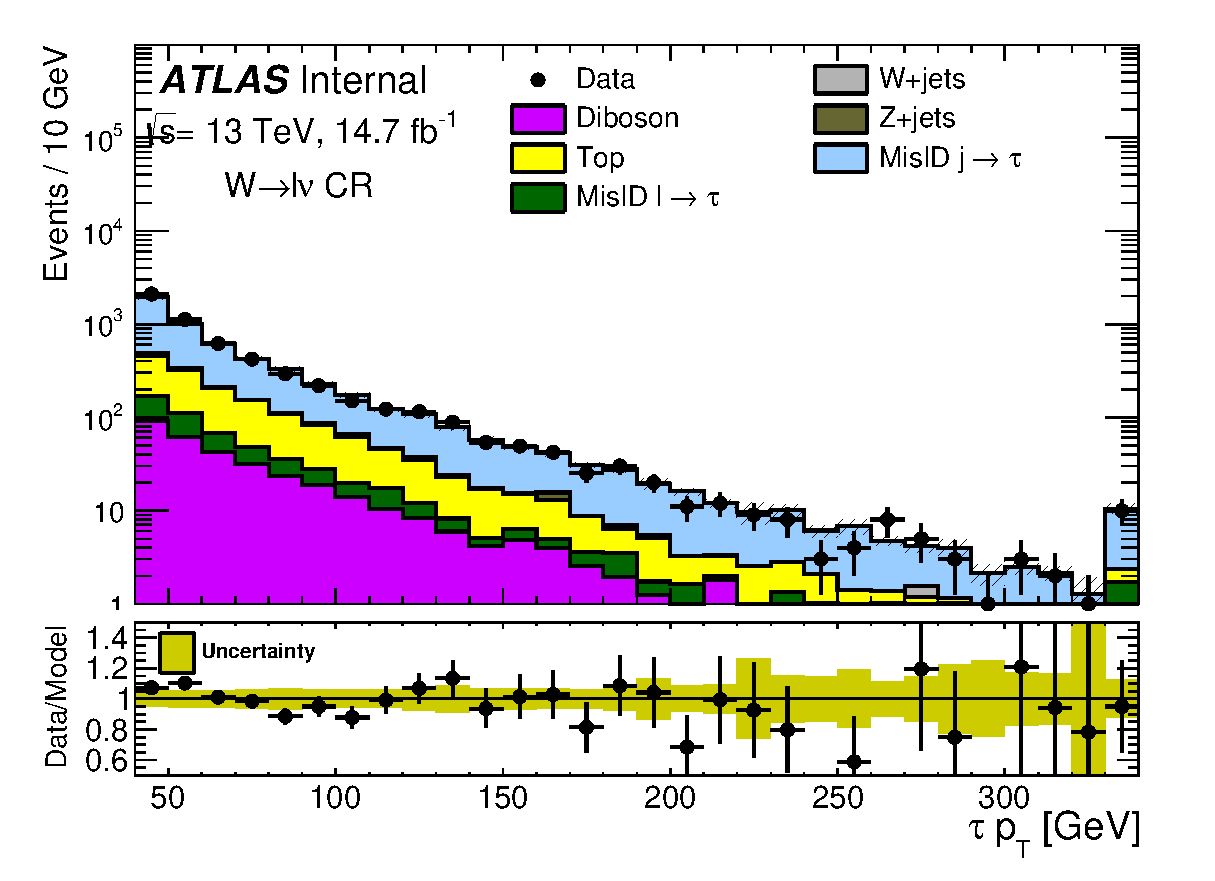
\includegraphics[width=\textwidth]{figures/DDQCD15_FFWCR_taupt_log.eps}
\caption{}
\end{subfigure} % 
\begin{subfigure}{0.5\textwidth}
   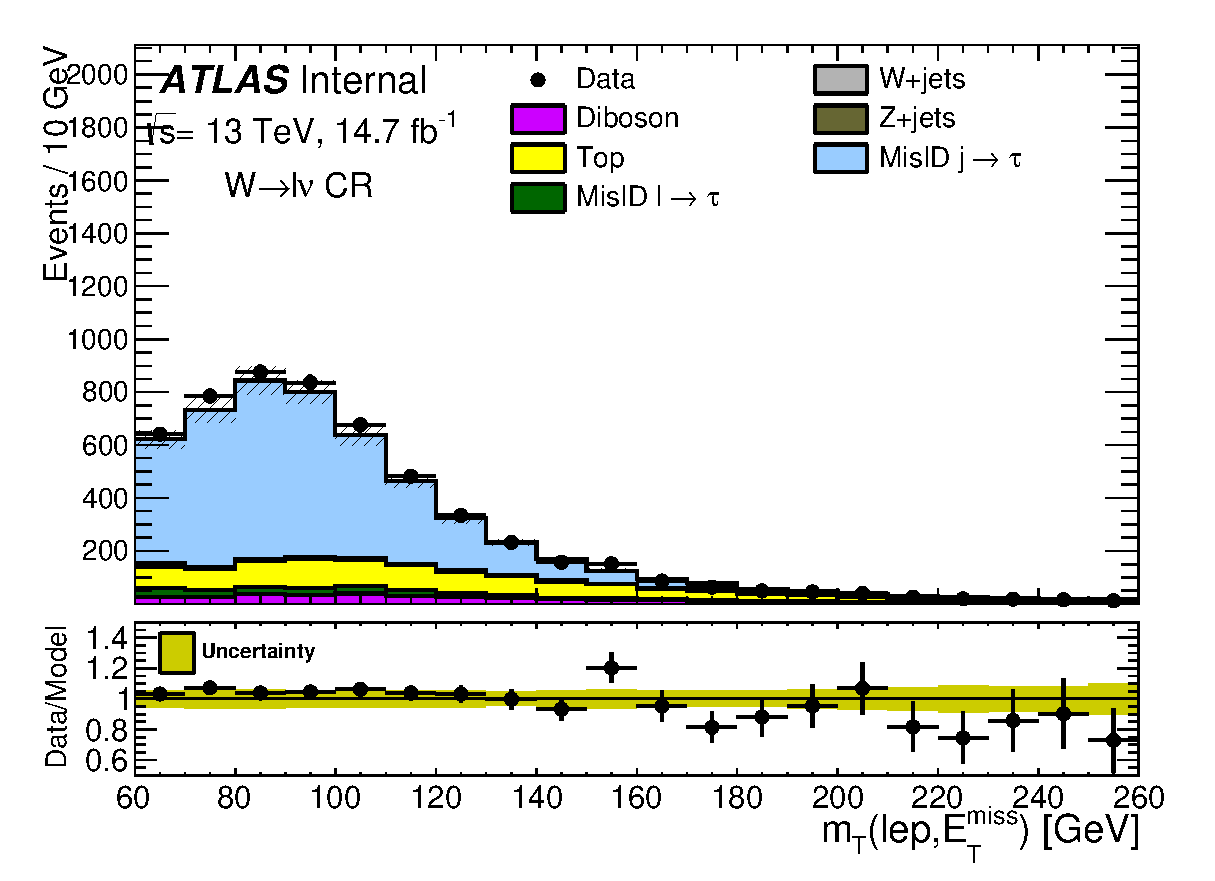
\includegraphics[width=\textwidth]{figures/DDQCD15_FFWCR_WlepMT.eps}
\caption{}
\end{subfigure}
\caption{\FF\ closure plots in the \Wjets\ control region}
\label{fig:clWjets}
\end{figure}

\begin{figure}[!h]
\begin{subfigure}{0.5\textwidth}
   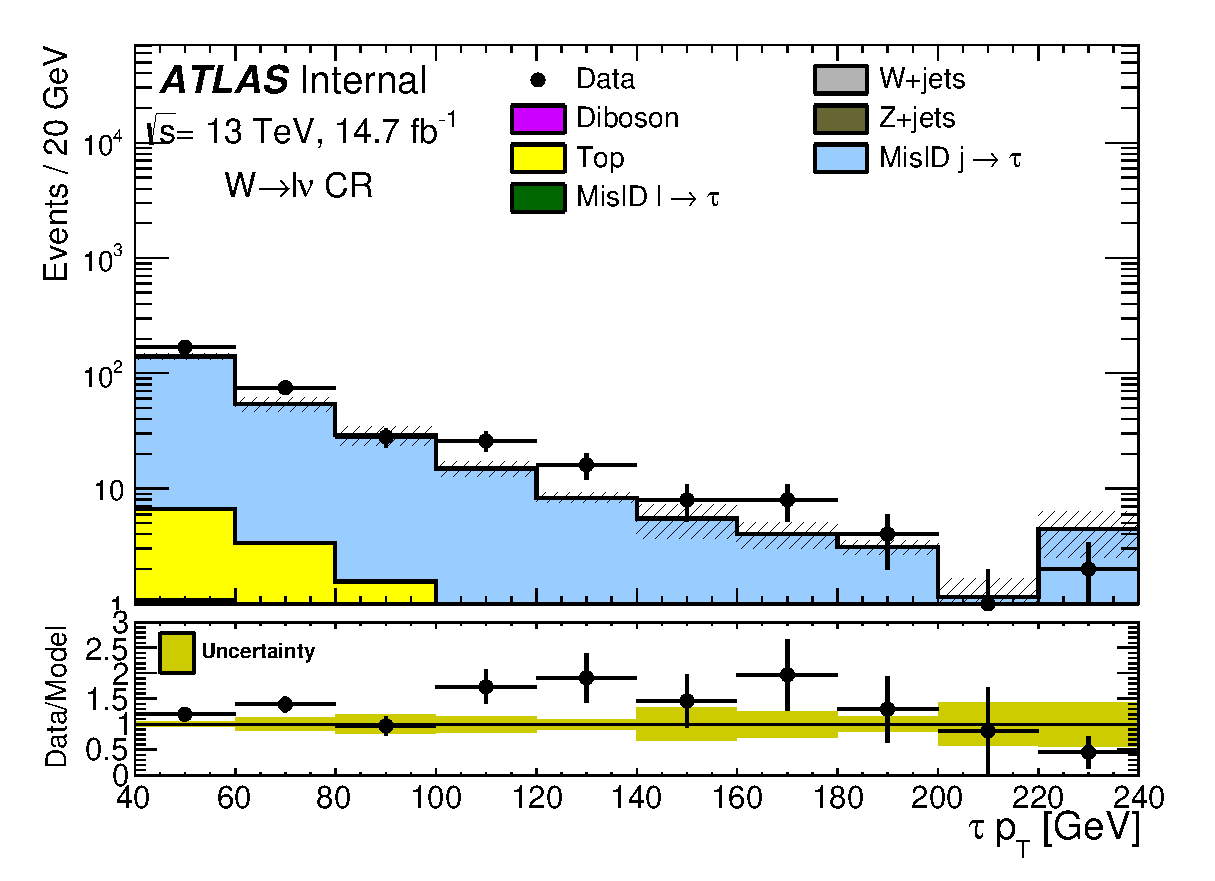
\includegraphics[width=\textwidth]{figures/DDQCD15_FFttll_taupt_log.eps}
\caption{}
\end{subfigure} % 
\begin{subfigure}{0.5\textwidth}
   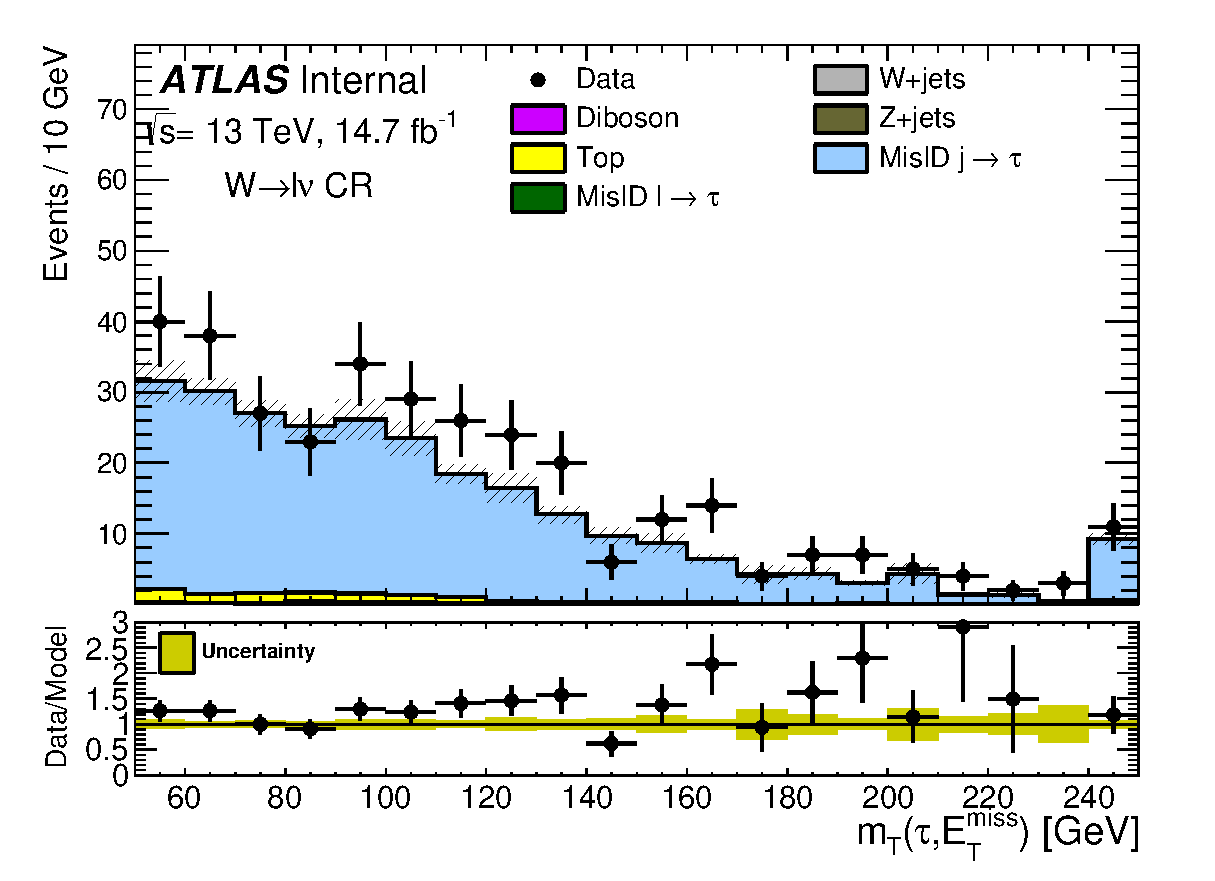
\includegraphics[width=\textwidth]{figures/DDQCD15_FFttll_MT.eps}
\caption{}
\end{subfigure}
\caption{\FF\ closure plots in the \ttbar\ control region}
\label{fig:clTTBar}
\end{figure}


\subsection{True $\tauvis$ backgrounds}
\label{sec:truetau}
\par True $\tauvis$ backgrounds are estimated from Monte Carlo simulation. 
Such backgrounds expected in the signal region are shown in Figures~\ref{fig:preselectA} and~\ref{fig:preselectB}.
Top and $\Wjets$ processes are expected to dominate these backgrounds, while a few $\Zboson+$jets and $VV$ 
events are also expected to contaminate the signal region.

\par \ttbar\ may be mis-classified as signal  
 when one of the top quarks decays leptonically as 

\begin{equation}
\begin{aligned}
t\to \Wplus b\to\tau\nu_\tau  &  & \text{and the other as,} \\
t\to \Wplus b\to qqb. &  &
\end{aligned}
\label{eq:ttBarDc}
\end{equation}

In this topology, the $\nu_\tau$  is reconstructed as $\met$ and the $\tau$ as $\tauvis$; the three quarks from the other 
top decay may be reconstructed as jets, one of which may be $b-$tagged.  
The $\mT(\tau,\nu_\tau)$, is usually 
low in this topology because the $\tauvis$ and \met\ are expected to be aligned in $\phi$. 
The secondary method of \ttbar signal contamination is when both top quarks decay 
leptonically and one of the leptons is not identified or reconstructed. In this case \mT\ is expected to be 
high because the \met\ is a reconstruction of two $\nu_\tau$.
A single top can get mis-classified as signal when the top quark decays leptonically, and the 
associated quarks are reconstructed as jets. Note that only the $Wt-$channel has multiple jets in the 
leading order calculation. So, contribution of single top to the signal region is relatively smaller than that 
of \ttbar. 

\par $\Wjets$ events enter the signal region when the $\Wplus$ decays to a $\tau$ lepton and a $\nu_\tau$. 
Since the signal region requires at least 3 jets in the event, \Wjets\ only enters the signal 
region if it has 3 or more associated jets.

\par Since \ttbar\ and \Wjets\ are the most dominant backgrouns processes in the signal region, 
dedicated control regions in data are devised to assess their modelling in simulation.   
For this assessment to be extrapolated to the signal region, these control regions 
are designed to be as close as possible to it. They are also designed to have as few signal events 
as possible to reduce bias.
 
\par The \ttbar\ control region differs from the signal region in that 2 or more $b-$tagged jets 
and $\mT<100$~\GeV\ are required. The $b-$tagged jets requirement is justifiable from Equation~\ref{eq:ttBarDc}. 
 The low $\mT$ selection is to maximize \ttbar\ events in which 
one of the top quarks decays to a $\tau$ lepton, while refraining from the high \mT\ region that is 
part of the signal region. With this selection criteria the \ttbar\ control region has a small 
overlap with the signal region, but the expected signal contamination is about one order of 
magnitude smaller than the expected fraction of \cHtaunu\ events in the signal region. Kinematic 
distributions in this region are shown in Figure~\ref{fig:ttBarCR}. 

\par The \Wjets\ control region differs from the signal region in that it requires events 
to have no $b-$tagged jets and have $mT<100$~\GeV. This region is orthogonal to the signal 
region, and yet close to the signal region in phase space. Kinematic variables are shown in 
Figure~\ref{fig:wjetsCR}.  

\begin{figure}[!h]
\begin{subfigure}{0.5\textwidth}
   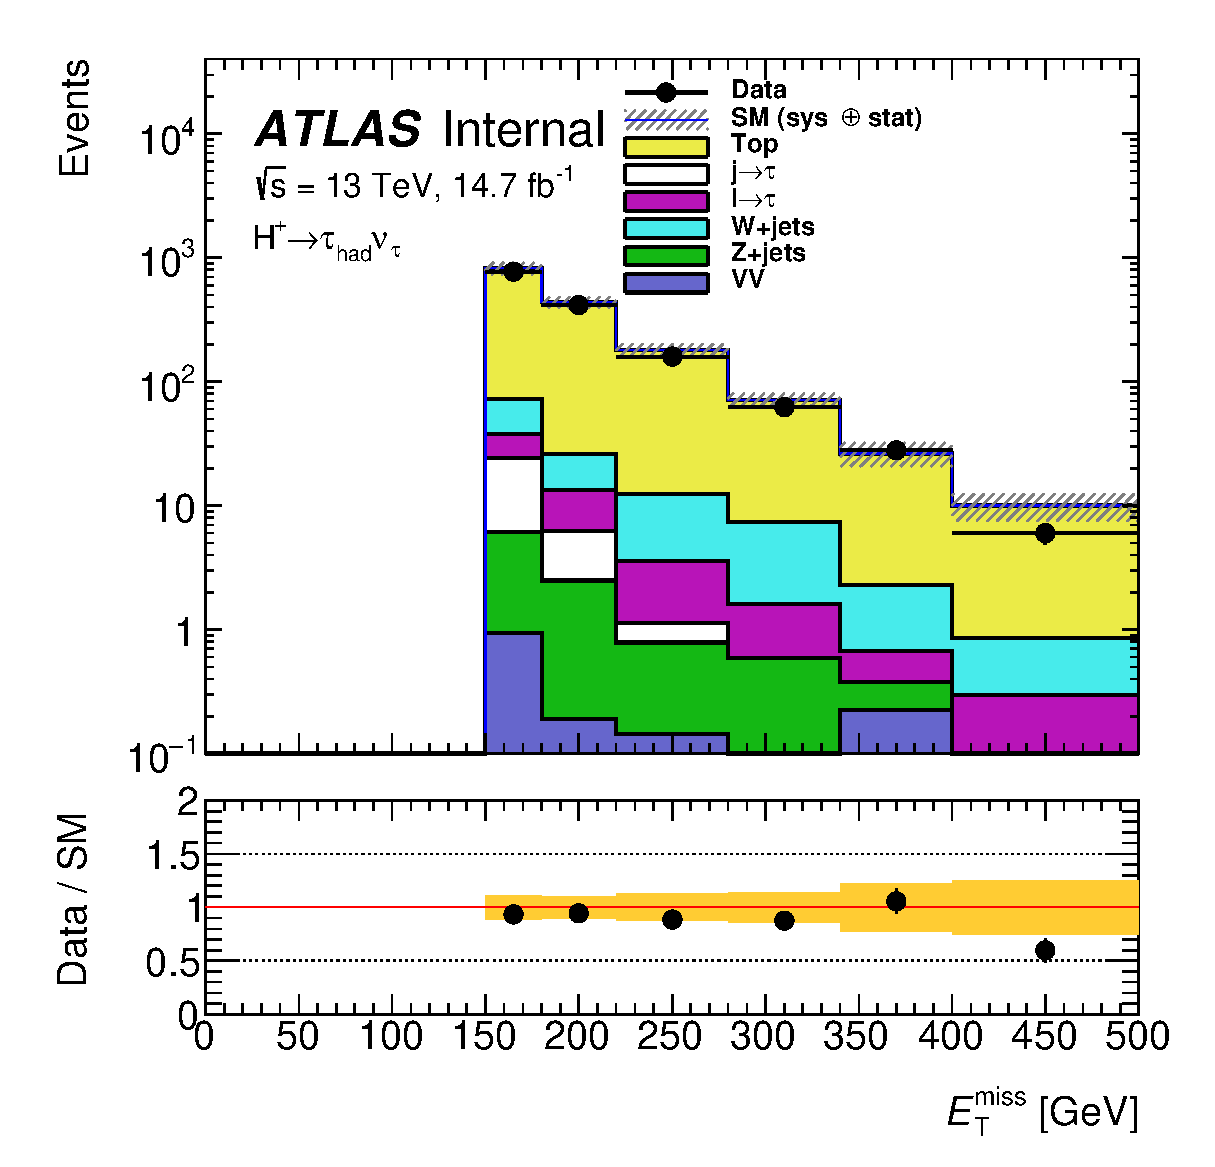
\includegraphics[width=\textwidth]{figures/met_TTBar.eps}
\caption{\met}
\end{subfigure} % 
\begin{subfigure}{0.5\textwidth}
   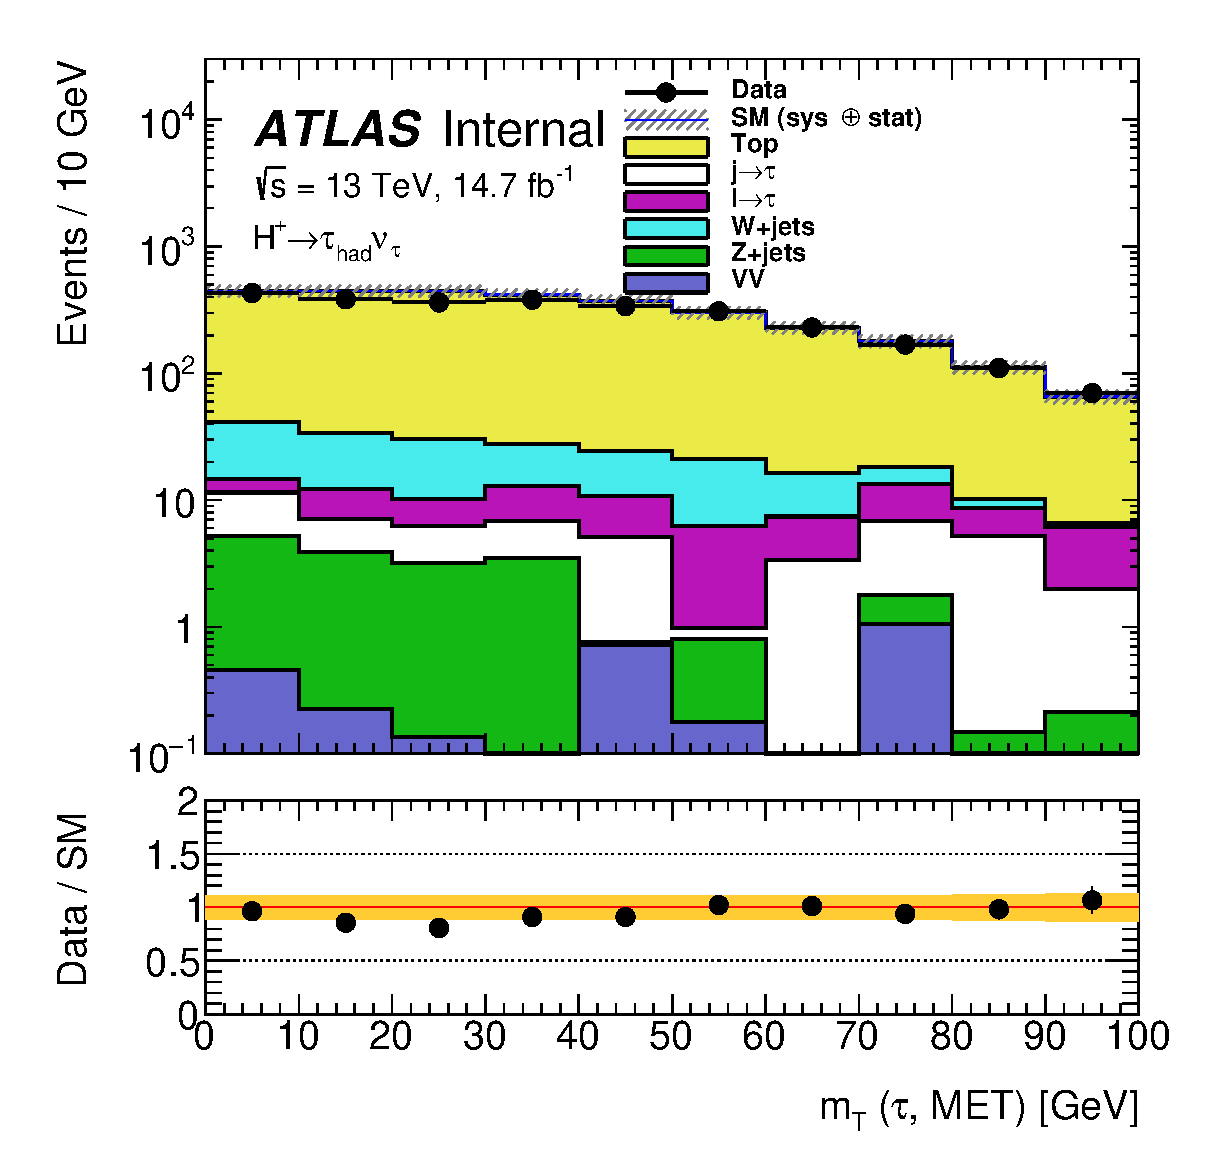
\includegraphics[width=\textwidth]{figures/mT_TTBar.eps}
\caption{\mT}
\end{subfigure}
\begin{subfigure}{0.5\textwidth}
   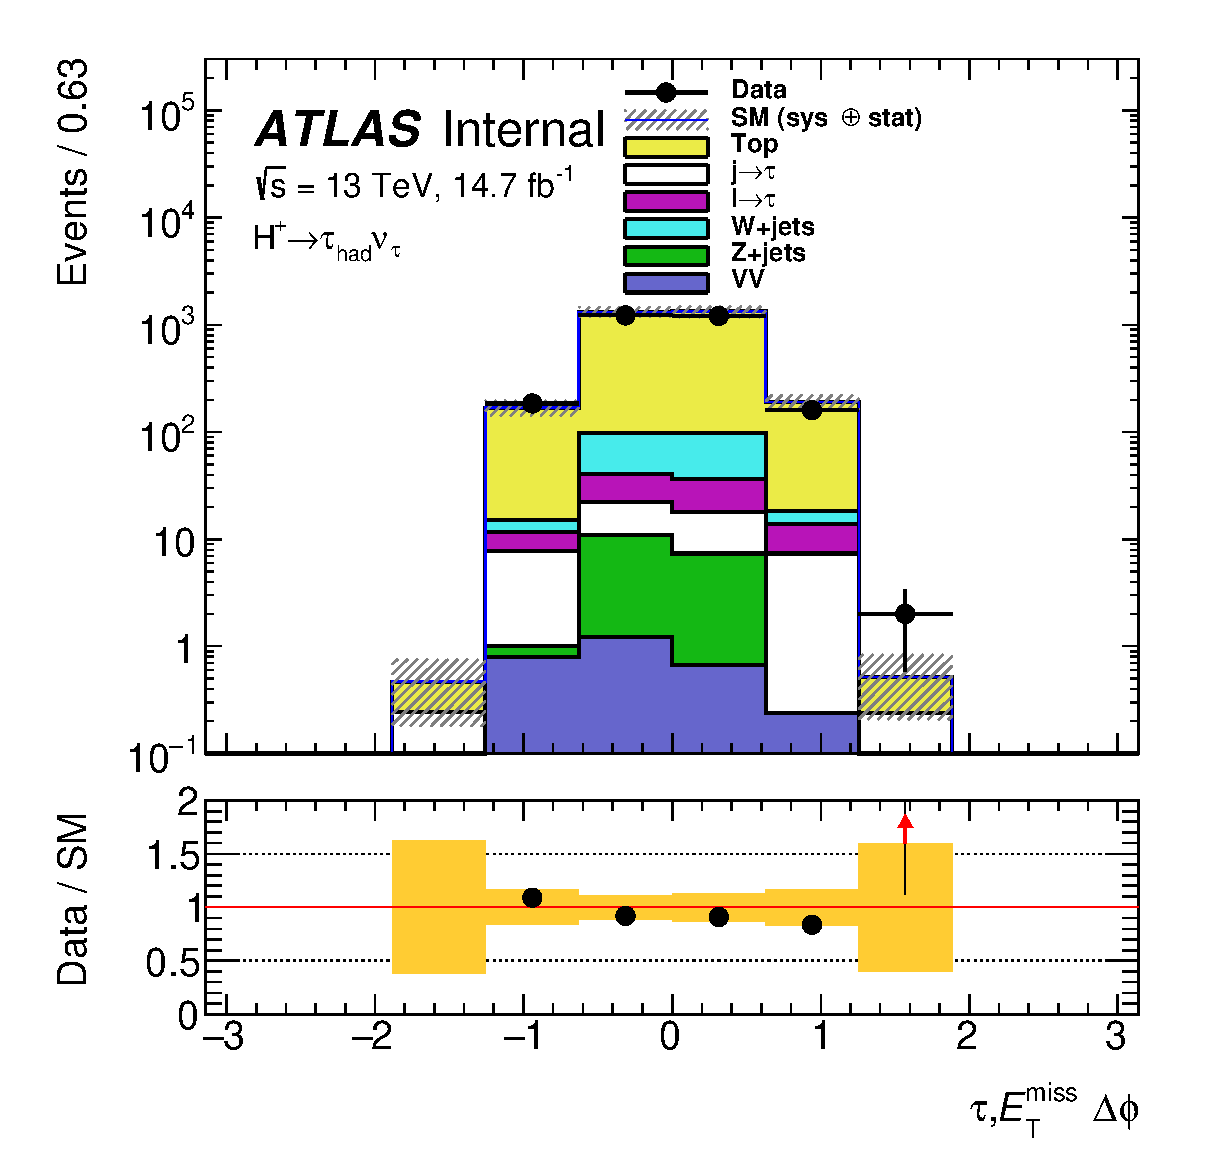
\includegraphics[width=\textwidth]{figures/taumetphi_TTBar.eps}
\caption{}
\end{subfigure} % 
\begin{subfigure}{0.5\textwidth}
   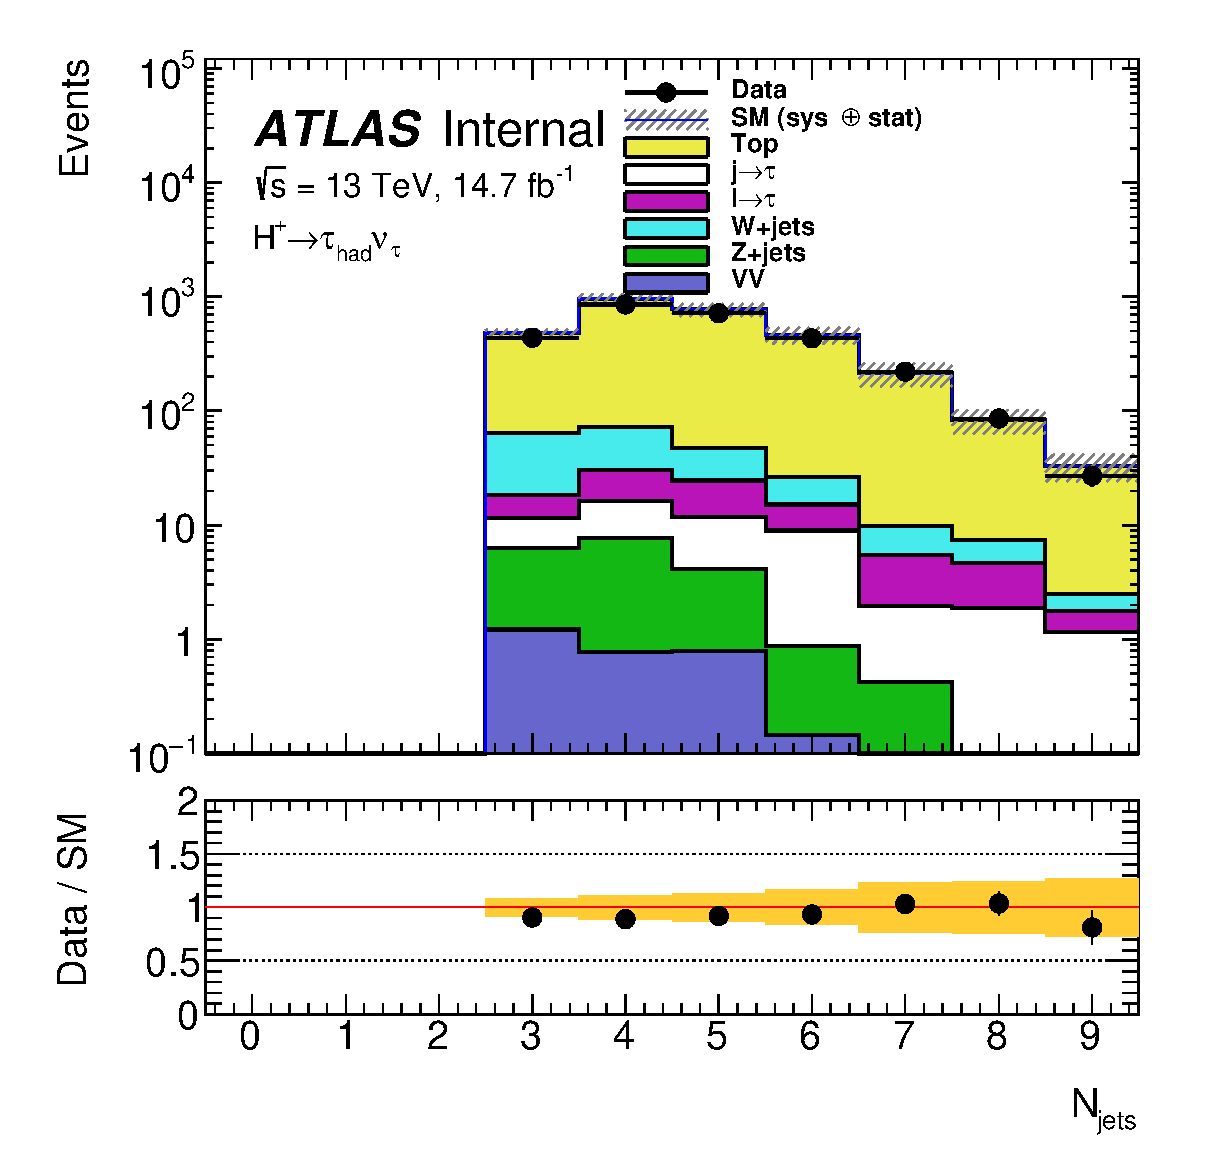
\includegraphics[width=\textwidth]{figures/nJets_TTBar.eps}
\caption{Number of jets}
\end{subfigure}
\caption{Plots showing kinematic distributions in the \ttbar\ control region}
\label{fig:ttBarCR}
\end{figure}

\begin{figure}[!h]
\begin{subfigure}{0.5\textwidth}
   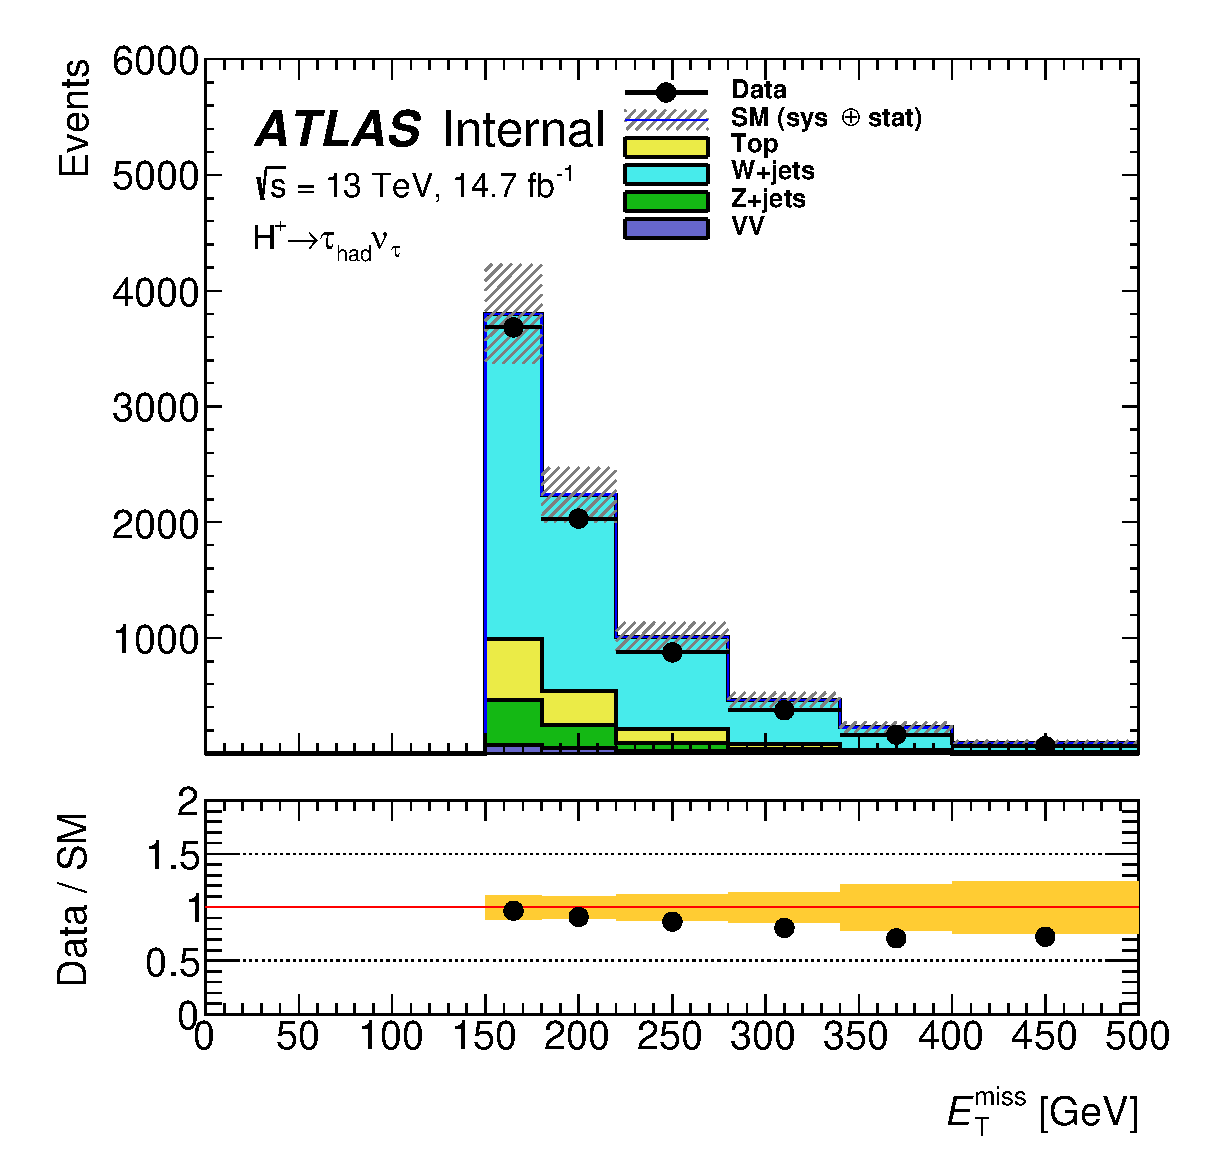
\includegraphics[width=\textwidth]{figures/met_Wjets.eps}
\caption{\met}
\end{subfigure} % 
\begin{subfigure}{0.5\textwidth}
   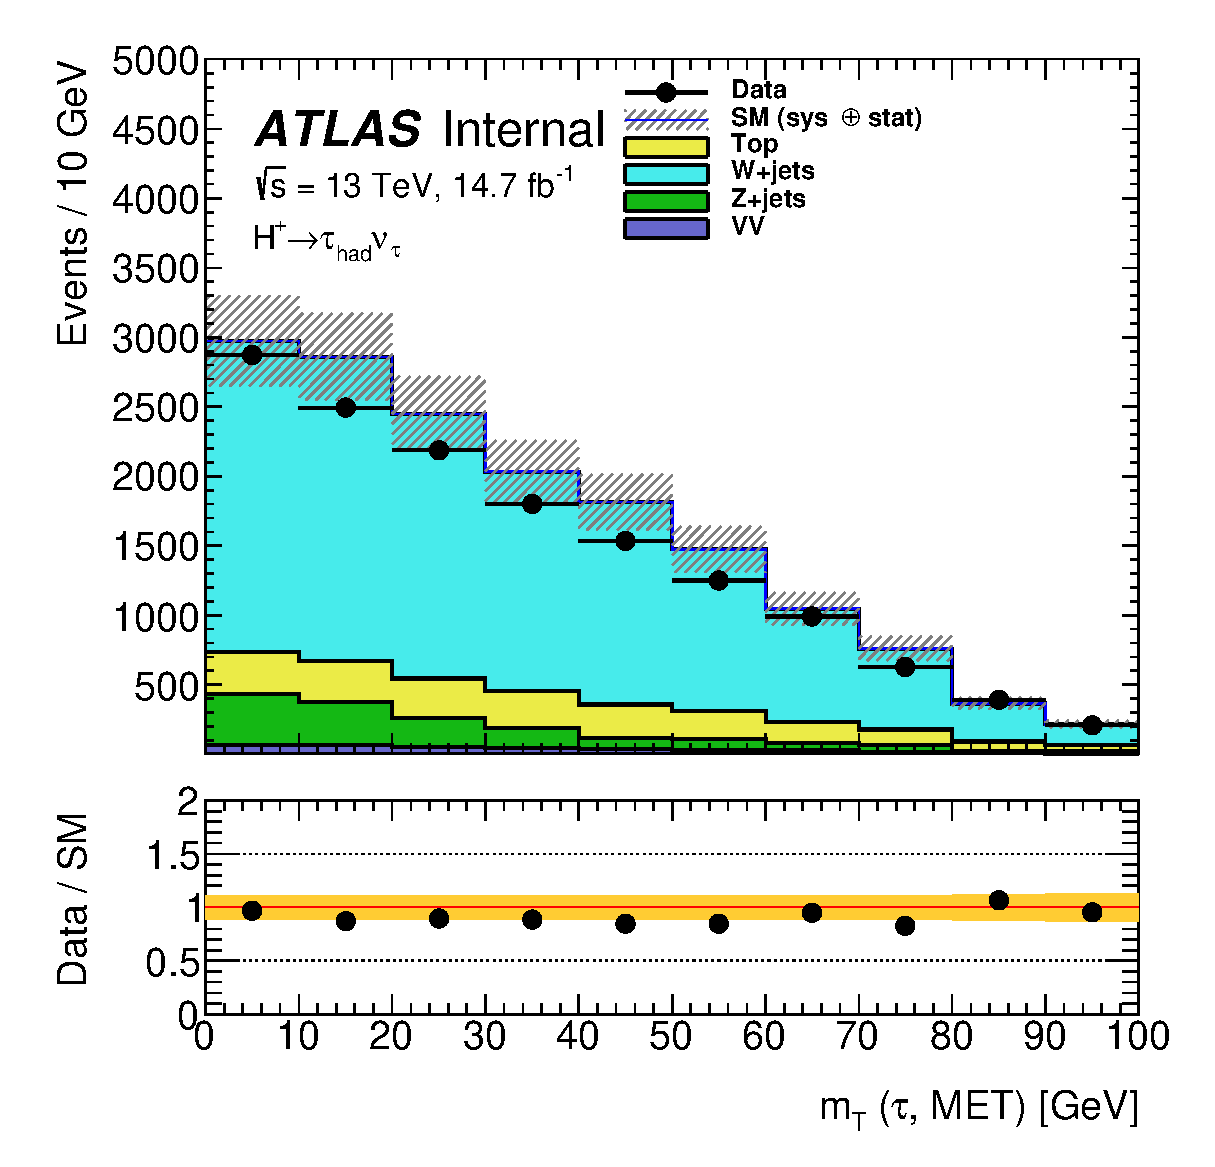
\includegraphics[width=\textwidth]{figures/mT_Wjets.eps}
\caption{\mT}
\end{subfigure}
\begin{subfigure}{0.5\textwidth}
   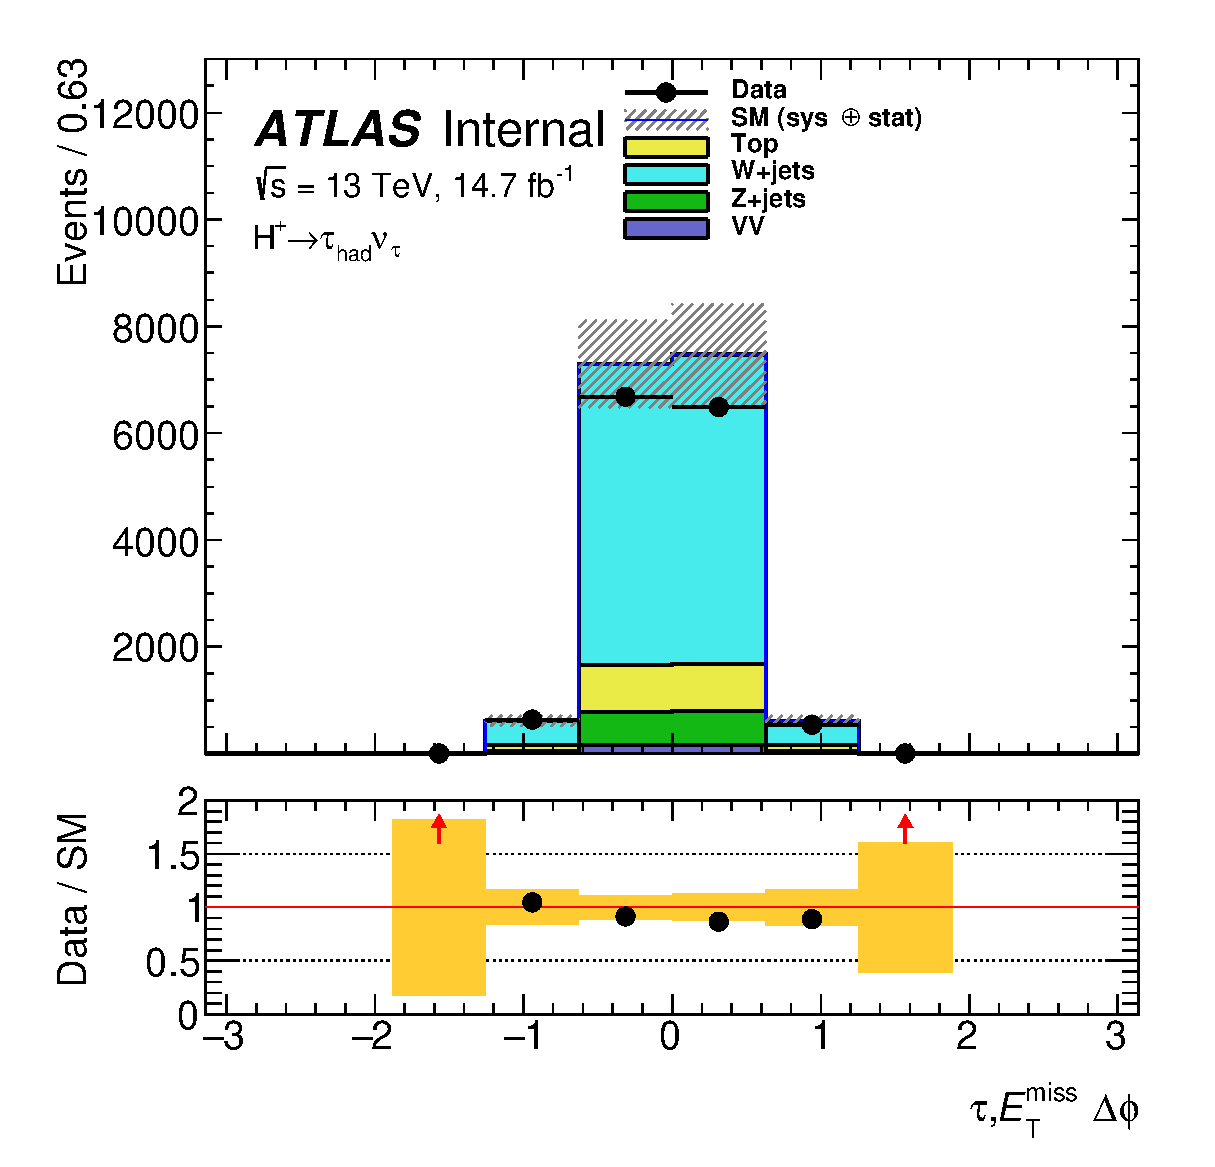
\includegraphics[width=\textwidth]{figures/taumetphi_Wjets.eps}
\caption{}
\end{subfigure} % 
\begin{subfigure}{0.5\textwidth}
   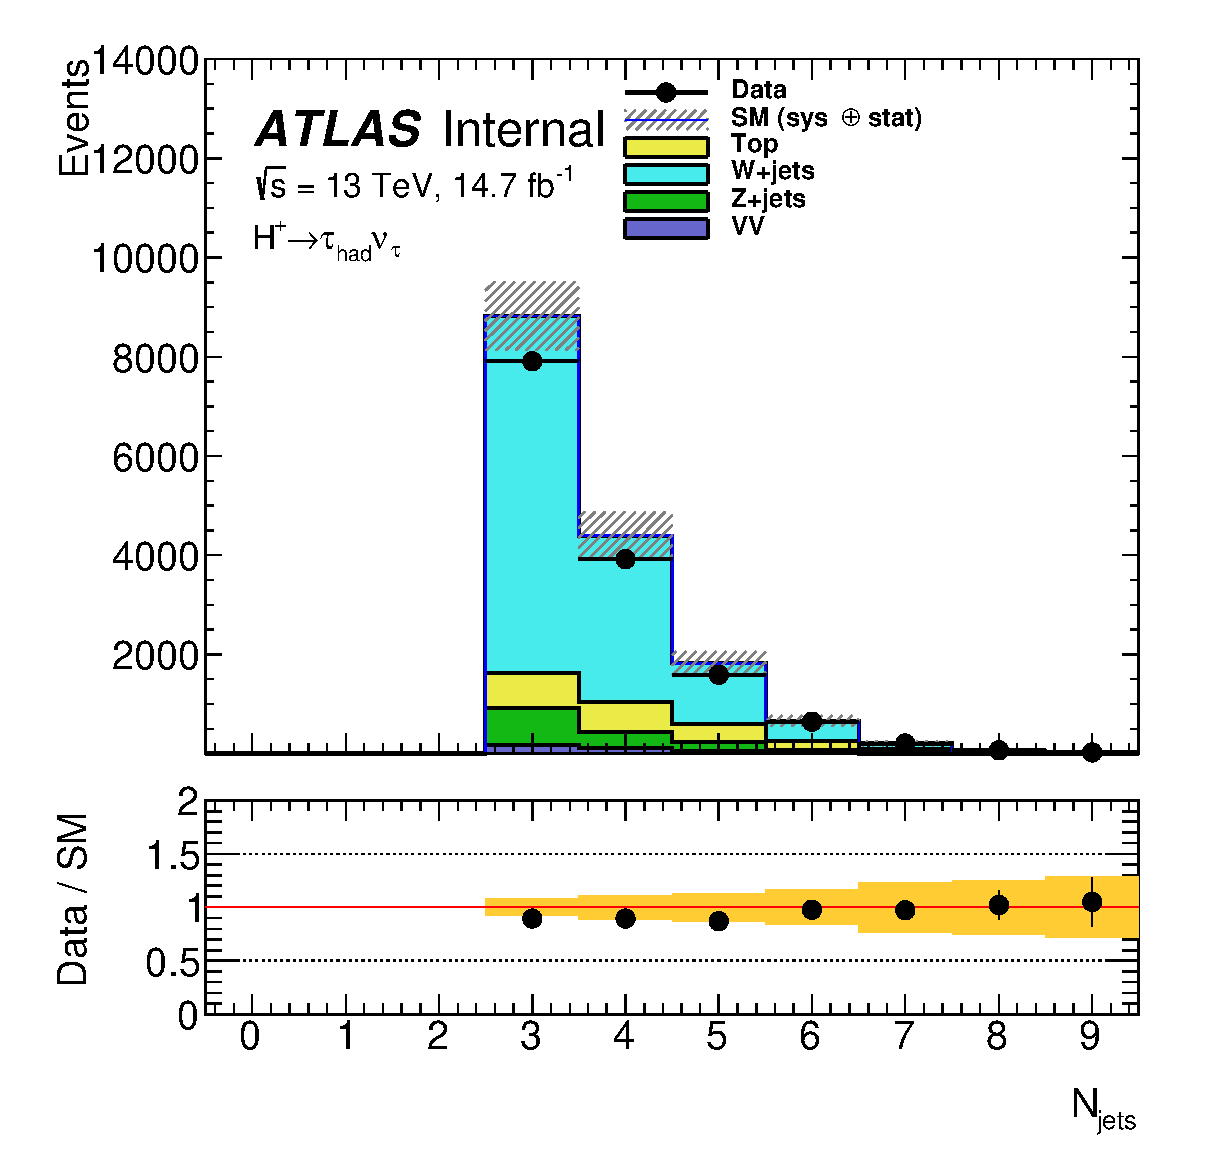
\includegraphics[width=\textwidth]{figures/nJets_Wjets.eps}
\caption{Number of jets}
\end{subfigure}
\caption{Plots showing kinematic distributions in the \Wjets\ control region}
\label{fig:wjetsCR}
\end{figure}



\section{Systematic Uncertainties and Statistical Methods}
\label{sec:systsCh}
\subsection{Systematic Uncertainties}
\label{sec:systsUnc}
\par Systematic uncertainities considered in this analysis are grouped into 
 experimental and theoretical categories. Regardless of the category, the procedure for evaluating 
each uncertainty's impact on the analysis results is the same:
\begin{enumerate}
\item  a parameter that corresponds to that uncertainty is shifted by $\pm 1\sigma$ from the 
nominal value; 
\item this shift may propagate to the final event yields, 
the shapes of key kinematic distributions such as \mT, or both; 
\item and finally, shape 
and yield shifts are both examined for each systematic variation in this analysis.  
\end{enumerate}

\subsubsection{Experimental Systematic Uncertainties}
\par Experimental systematic uncertainties include uncertainties on reconstruction efficiencies, 
identification efficiencies, energy scales, or momentum scales of all the physics objects 
used in the analysis. These objects are electrons, jets, and the \tauvis. These variations were propagated 
to the hard term component of \met. An additional uncertainty was also considered on the \met\ soft 
term. The uncertainty due to $b$-tagging efficiency was also considered. Table~\ref{tab:expUnc} 
shows the impact of the most dominant uncertainties on \ttbar\ and several of the expected yields. 
Uncertainties related to electrons and muons were found to be negligibly small. 

\begin{table}[!h]
\begin{center}
  \resizebox{\textwidth}{!}{
\begin{tabular}{|l|cc|cc|cc|cc|}
\hline
\multirow{2}{*}{Variation} & \multicolumn{2}{c|}{\ttbar}& \multicolumn{2}{c|}{Signal $\mcH=400~\GeV$}   & \multicolumn{2}{c|}{Signal $\mcH=1000~\GeV$} & \multicolumn{2}{c|}{Signal $\mcH=2~\TeV$}  \\
													 & up (\%) & down (\%)       & up (\%) & down (\%)       &up (\%) & down (\%)       &up (\%) & down (\%)       \\
\hline\hline
\tauvis\ reconstruction efficiency & -2.8 & 2.8 & 2.4 & 2.4 & -2.1 & 2.1 & -2.2 & 2.2 \\
\tauvis\ ID efficiency & -11.2&11.2 & -7.7& 7.7 & -7.3 & 7.3 & -8 & 8 \\
\tauvis-lepton OLR & -1.2 & 1.2 & -1.7 & 1.7 & -2.3 & 2.3 & -2.4 & 2.4 \\
\tauvis\ energy scale & -6.4 & 6.1 & -4.8 & 4.0 & -1.2 & 1.5 & 1.8 & -0.4 \\
\hline 
Jet energy scale & -10 & 11 & -4.4 & 4.8 & -1.8 & 2.6 & -1.1 & 1.9 \\
$b-$tagging efficiency & -2 & 2 & 2 & -2 & 1.7 & -1.6 & 1.5 & -1.5 \\
\met\ soft term scale/resolution & $2.1$ & $-2.1$ & -1.6 & 1.6 &  $<0.1$ & $<0.1$ &  $<0.1$ & $<0.1$ \\
Trigger efficiency & -3 & 3 & -1 & 1 & 0.2 & 0.2 &  $<0.1$ & $<0.1$ \\ 
\hline
\end{tabular}
}
\end{center}
\caption{Experimental systematic uncertainties.}
\label{tab:expUnc}
\end{table}


\par The procedures for obtaining systematic uncertainties for \tauvis, jet and b-tagging are 
discussed in Chapter~\ref{obj}.   

\par The systematic uncertainty associated with the trigger efficiency is a combination of the following 
uncertainties :
\begin{enumerate}
\item statistical uncertainties in each bin of the efficiency distribution; 
\item identification of \tauvis\ in the control region used to measure the trigger efficiency;
\item identification of the electron in the said control region; 
\item and jet reconstruction in the said control region. 
\end{enumerate}  

Statistical uncertainties in each bin of the turn-on curve are assummed to follow a Poisson 
distribution. Identification of the \tauvis\ was evaluated by varying its identification 
criteria from loose to medium, and tight. The same variation technique was applied to 
the electron object. The number of reconstructed jets requirement was varied between a minimum 
of two and three. %The effect of these variations is shown in Figure~\ref{fig:trigVars}

\par Uncertainties associated with fake factors, described in Section~\ref{sec:jetToTau}, were also 
 observed to be significantly large. 
As already mentioned, the object from which the reconstructed jet is initiated (light flavor 
quark, heavy flavor quark or gluon) affects the values of the measured fake factors. The minimum 
jet BDT score required for jets in the anti-$\tau$-id region was varied to allow different composition 
of reconstructed jets. Since the nominal selection is 0.5, the $\pm 1\sigma$ variations were taken 
as 0.4 and 0.6 respectively. These variations affect both the shape of the \mT\ distribution in 
the signal region, and the overall yield of accepted events. The effect on the latter is about 20\%. 
The effect of the former is shown in Figure~\ref{fig:bdtFF}. 
The number of \tauvis\ matched to true $\tau$ leptons in $N^{\text{anti-}\tau}_{\text{fakes}}$, when 
computing $N^{\tau}_{\text{fakes}}$ in Equation~\ref{eq:ffDef} was also generously varied by 50\%. 
This variation affects both the shape of the \mT\ distribution in the signal region and the final 
accepted event yield. The latter is shifted by about 6\%. The last significant source  of uncertainty in 
the fake factor method is due to statistical uncertainties in the measurement control samples. This only 
affects the event yield by about 3\%. No \mT\ shape shifts were observed.   

\begin{figure}[!h]
\centering
   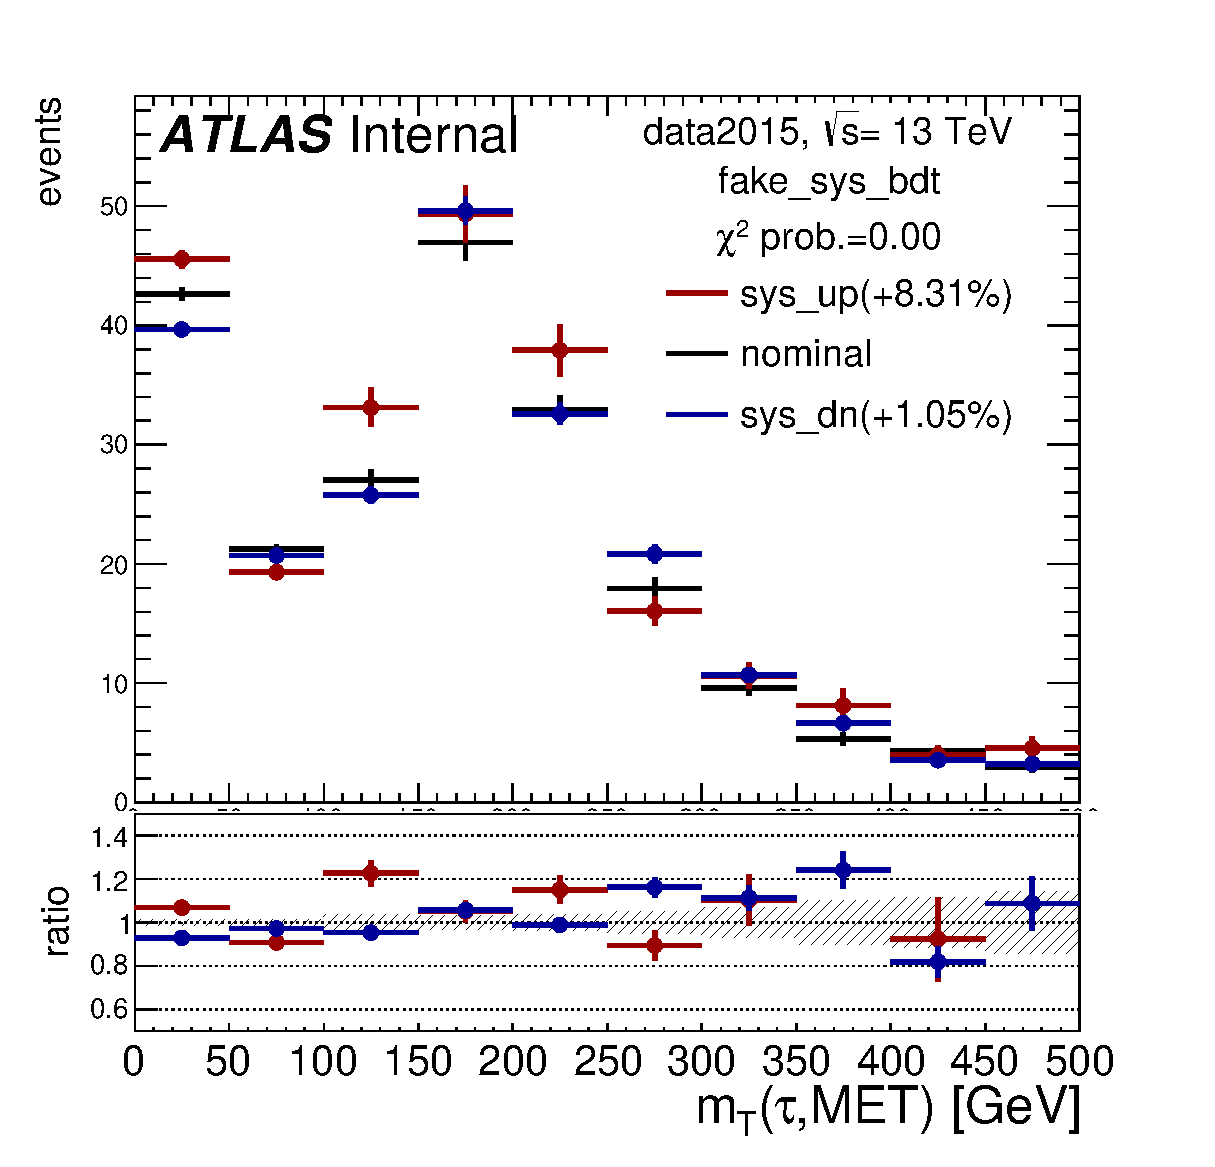
\includegraphics[width=0.8\textwidth]{figures/Syst_fake_sys_bdt.eps}
\caption{Plots showing \mT\ distributions with variation in jet BDT score selection criteria}
\label{fig:bdtFF}
\end{figure}

\subsubsection{Theoretical Systematic Uncertainties}
\par Theoretical uncertainties include uncertainties due to the choice of the QCD renormalization
 and factorization scales, choice of parton distribution functions, and tunes applied to the parton 
shower and underlying event models. These uncertainties were computed for signal samples and the most 
dominant backgrounds, which are \ttbar\ and \Wjets.    

\par For signal samples, the QCD renormalization scale $\mu_R$ and factorization scale $\mu_F$ were 
varied by a factor of 0.5 and 2.0 to evaluate their impact on the expected signal yields. 
This impact was shown to be less than 5\%. Table~\ref{tab:scalesSig} shows the percentage impact 
on the individual variations on several \mcH.  The largest variation was symmetrized and 
taken as the QCD scale uncertainty for that mass point.  

\begin{table}[!h]
\begin{center}
  \resizebox{\textwidth}{!}{
\begin{tabular}{|l|cccccccc|}
\hline
Mass  & \multicolumn{8}{c|}{$\mu_R\times\mu_F$ (\% diff)}  \\
(GeV) & $0.5\times0.5$ &  $0.5\times1.0$ & $0.5\times2.0$ & $1.0\times0.5$ & $1.0\times2.0$ & $2.0\times0.5$ & $2.0\times1.0$ & $2.0\times2.0$ \\
\hline\hline
200 & -8 & 1.7 & 7 & -7 & 4 & -8 & -2 & 2 \\
500 & -5 & -1 & 2 & -3 & 2 & -2 & 1 & 2 \\
800 & -4 & -1 & 1 & -2 & 1 & -1 & 1 & 2 \\
1000 & -4 & -1.3 & 0.6 & -2 & 1.5 & 0.7 & 1 & 2 \\
\hline
\end{tabular}
}
\end{center}
\caption{Theoretical systematic uncertainties on the signal acceptance (in \%) due to the QCD scale. 
The factorization scales are varied by a factor of 2 for up and down variations.}
\label{tab:scalesSig}
\end{table}

\par Dependence on the parton distribution function (PDF) set choice is evaluated by LHAPDF~\cite{Buckley:2014ana}. 
For a sample generated with PDF set $A$, LHAPDF is able to compute weights for each event, such that
the dataset would equivalent to a dataset generated with PDF set $B$. By taking NNPDF23\_nlo\_as\_0118\_qed 
 as the nominal PDF set, 3 variations were then examined : NNPDF30\_nlo\_as\_0118\_nf\_4, 
CT14nlo\_NF4, and MSTW2008nlo68cl\_nf4. The largest variation was symmetrized and taken as the error 
on the PDF choice. This variation was found to have less than 1\% impact on the results 
for all signal samples.  

\par Uncertainties due to parton shower and underlying event tunes were considered for 
$\mcH=200, 500,$ and 800~\GeV. The A14 tune with the NNPDF set comes with a set of 
systematic variations that were empirically found to cover the total uncertainty in the data used to 
tune parton shower and underlying event models. A pair of these variations, {\it Var1}, covers 
underlying event effects. Another pair, {\it Var2}, covers jet structure effects. 3 other pairs, {\it Var3a, Var3b} and 
{\it Var3c}, cover aspects of extra jet production. The up and down variations were symmetrized and summed in quadrature to obtain 
their full impact. Table~\ref{tab:systsPS} summarizes the percentage impact of each symmetrized variation. 

\begin{table}[!h]
\begin{center}
\begin{tabular}{|l|ccccc|}
\hline
Mass (GeV)  & Var1 (\%) & Var2 (\%)& Var3a (\%) & Var3b (\%) & Var3c (\%)  \\
\hline\hline
200 & 2 & 7 & 8 & 10 & 10 \\
500 & 4 & 4 & 5 & 4  & 6  \\
800 & 4 & 4 & 5 & 8 & 1 \\
\hline
\end{tabular}
\end{center}
\caption{Theoretical systematic uncertainty on the signal acceptance due to choice of parton shower and 
underlying event tune.}
\label{tab:systsPS}
\end{table}

\par QCD scale, choice of parton shower and underlying event tunes, and choice for matrix element generator 
were evaluated for \ttbar. The impact on the predictions was evaluated by generating Monte Carlo simulation samples    
with the respective variations and imposing signal region selection criteria on them. 
 \POWHEG+\PYTHIA\ version 8 
samples were used as the nominal samples. Separate samples with more final state radiation (FSR) and 
less FSR were also generated. \MGMCatNLO+\HERWIGPP\ and \POWHEG+\HERWIGPP\ samples 
were generated to evaluate the impact of using different matrix element generators.    
The impact of using different parton showering and underlying event tunes was computed 
by comparing \POWHEG+\PYTHIA version 8 and \POWHEG+\HERWIGPP samples. QCD scale and PDF choice 
uncertainties were shown to be less than 5\%. Shift on the event yield due to FSR was shown to be 
approximately 7\%, for the choice of matrix element generator it was 15\%, and for the choice of 
parton shower and underlying event tunes it was 16\%. Effects of these variations on the shape 
of the $\mT(\tau,\nu)$ distribution were also examined, after normalizing the samples to the same 
NNLO+NNLL cross section.% Figures~\ref{fig:shapeTTBarA}, \ref{fig:shapeTTBarB}, \ref{fig:shapeTTBarC}
% shows these shape differences.    

\par Various selection criteria in the \Wjets\ control region were varied to evaluate the 
systematic uncertainties on the \Wjets\ background. All these variations were shown to be 
less than 3\%. Since contributions from other background process in the signal region are 
very small, their systematic variations were taken as negligible. 

\subsection{Statistical Methods}
\par The \mT\ distributions for signal samples with $200<\mcH<2000~\GeV$, and background processes
 in the signal region are used to test for the presence of charged Higgs bosons with \mcH\ in the 200$\to$2000~\GeV mass range 
in data. This procedure involves tests on two hypotheses : that the data is fully 
described by the known Standard Model processes, called the {\it background-only} ($b$) hypothesis; and that some 
signal is required to explain the observed data, called the {\it signal+background} ($s+b$) hypothesis. 
Since the signal true cross section $\sigma_{H^+}^{Obs}$ is not known a-priori, a parameter of interest (POI)  

\begin{equation}
\mu = \frac{\sigma_{H^+}^{Obs}}{\sigma^{Exp}_{H^+}}
\end{equation}

is defined to parametrize the $s+b$ hypothesis into $\mu.s+b$. Here, $\sigma^{Exp}_{H^+}$ is the 
expected cross section from phenomenological models introduced in Chapters~\ref{theory}. A test can be made independent of 
$\sigma^{Exp}_{H^+}$ by setting it equal to 1; this would make the POI $\mu$ equal to the true 
cross section $\sigma_{H^+}^{Obs}$. In any case $\mu\geq 0$, where $\mu=0$ reduces the $s+b$ hypothesis to the 
background-only hypothesis. 

\par Since the number of events in the signal region is usually small, the \mT\ distributions used  for these 
tests are optimally binned to minimize statistical uncertainties. For an \mT\ distribution with $N$ bins, 
the expected number of events in each bin can be parametrized as   

\begin{equation}
E_i = \mu.s_i + b_i
\end{equation} 

where $i$ runs from 0 to $N$. Variables $s_i$ and $b_i$ are the expected signal 
and background events in the $i-$th bin respectively. These events follow a Poisson probability distribution 
with means $s_i$ and $b_i$ respectively. The statistical methods described here are based on the {\it binned likelihood 
function, L}, which is a product of Poisson probability terms over all the $N$ bins    

\begin{equation}
L(\mu) = \prod_{i=0}^N \frac{(E_i)^{n_i}}{n_i!}\exp (-E_i)
\end{equation}

\par $s_i$ and $b_i$ are affected by the systematic uncertainties discussed in Section~\ref{sec:systsUnc}. 
More specifically, the $s_i$ and $b_i$ probability distributions become wider when the systematic uncertainties 
are accounted for. A set of $P$ systematic uncertainties can be included in the statistical 
method as {\it nuisance parameters}, $\theta = (\theta_1,...,\theta_P)$, transforming $s_i$ and $b_i$ 
as $s_i\to s_i(\theta)$ and $b_i\to b_i(\theta)$ respectively.   
Likewise, the binned likelihood function is transformed as  

\begin{equation}
L(\mu) \to L(\mu,\theta) = \prod_{i=0}^N \frac{(\mu.s_i(\theta) + b_i(\theta))^{n_i}}{n_i!}\exp(\mu.s_i(\theta) + b_i(\theta)).\prod_{k=1}^P\rho(\theta_k).
\end{equation}

\par From the binned likelihood function a test statistic called the {\it profile likelihood ratio}

\begin{equation}
q_\mu = -2\ln\left (\frac{L(\mu,\hat{\hat{\theta}}}{L(\hat{\mu},\hat{\theta})} \right )
\label{eq:testStat}
\end{equation}

is created, where $\hat{\mu}$ and $\hat{\theta}$ are parameters that maximize the likelihood functions. 
The $\hat{\hat{\theta}}$ parameters are the nuisance parameters that maximize the likelihood function for a given $\mu$ value. 
 
\par The compatibility between data and a given hypothesis is quantified by computing a $p$-value. 
This is the probability of observing results as incompatible with data or worse, given that said hypothesis. 
For the $s+b$ hypothesis, the $p$-value is 
 
\begin{equation}
p_{s+b} = \int_{q_{\text{obs}}}^{\infty} f(q|s+b)dq
\label{eq:sPb}
\end{equation}

where $f(q|s+b)$ is the probability distribution function of the test statistic $q$ given the $s+b$ 
hypothesis. For the $b$ hypothesis the $p$-value is 

\begin{equation}
p_{b} = \int_{q_{\text{obs}}}^\infty f(q|b)dq
\label{eq:b}
\end{equation}

where $f(q|b)$ is the probability distribution function of the test statistic $q$ given the $b$ 
hypothesis. Figure~\ref{fig:pVal} illustrates how these $p_{b}$ is computed from a distribution 
of $f(q|b)$ and an observed $q_{\text{obs}}$ in data. 

\par These $p$-values are converted to a {\it significance}, defined as the number 
of standard deviations $Z$ at which a normally distributed variable with 0 mean would give a 
one-sided tail area equal to the $p-$value. %Figure~\ref{fig:zscore} illustrates the relationship 
%between $Z$ and $p$.   

\begin{figure}[h]
\centering
   \includegraphics[width=0.8\textwidth]{figures/pVal_sPb.pdf}
\caption{$p_{b}$ illustration from a distribution 
of $f(q|b)$ and an observed $q_{\text{obs}}$ in data}
\label{fig:pVal}
\end{figure}

\par From Equations~\ref{eq:sPb} and \ref{eq:b} a confidence level (CL) of the $s+b$ hypothesis is 
defined as 
 
\begin{equation}
CL_s(\mu) = \frac{CL_{s+b}}{CL_b} = \frac{p_{s+b}}{1-p_b}
\label{eq:cls}
\end{equation}

A 95\% CL upper limit on $\mu$ is set by finding the $\mu$ at which $CL_s = 0.05$, using the 
asymptotic approximation. 


\section{Results}
\label{sec:resCh}
\subsection{Expected and Observed Event Yields}
\par After all background processes have been estimated, and their associated systematic 
uncertainties have been evaluated, final kinematic distributions in the signal region were 
examined. Figure~\ref{fig:primSR} shows such n-1 distributions for \met\ and \mT. The black vertical 
lines show the values at which the selection criteria for the plotted variables were imposed.
 The yellow band in the ratio plot encodes the overall systematic and statistical uncertainties, 
summed in quadrature. In Figure~\ref{fig:primSR} this band is shown only in  
the signal region because that is where the systematic uncertainties were evaluated.        
Table~\ref{tab:yieldsSR} shows the expected event yields from background processes and 
the observed yield from 14.7~\ifb of data, accumulated during the 2015 and 2016 data taking 
periods. 

\begin{figure}[!h]
\begin{subfigure}{0.5\textwidth}
					 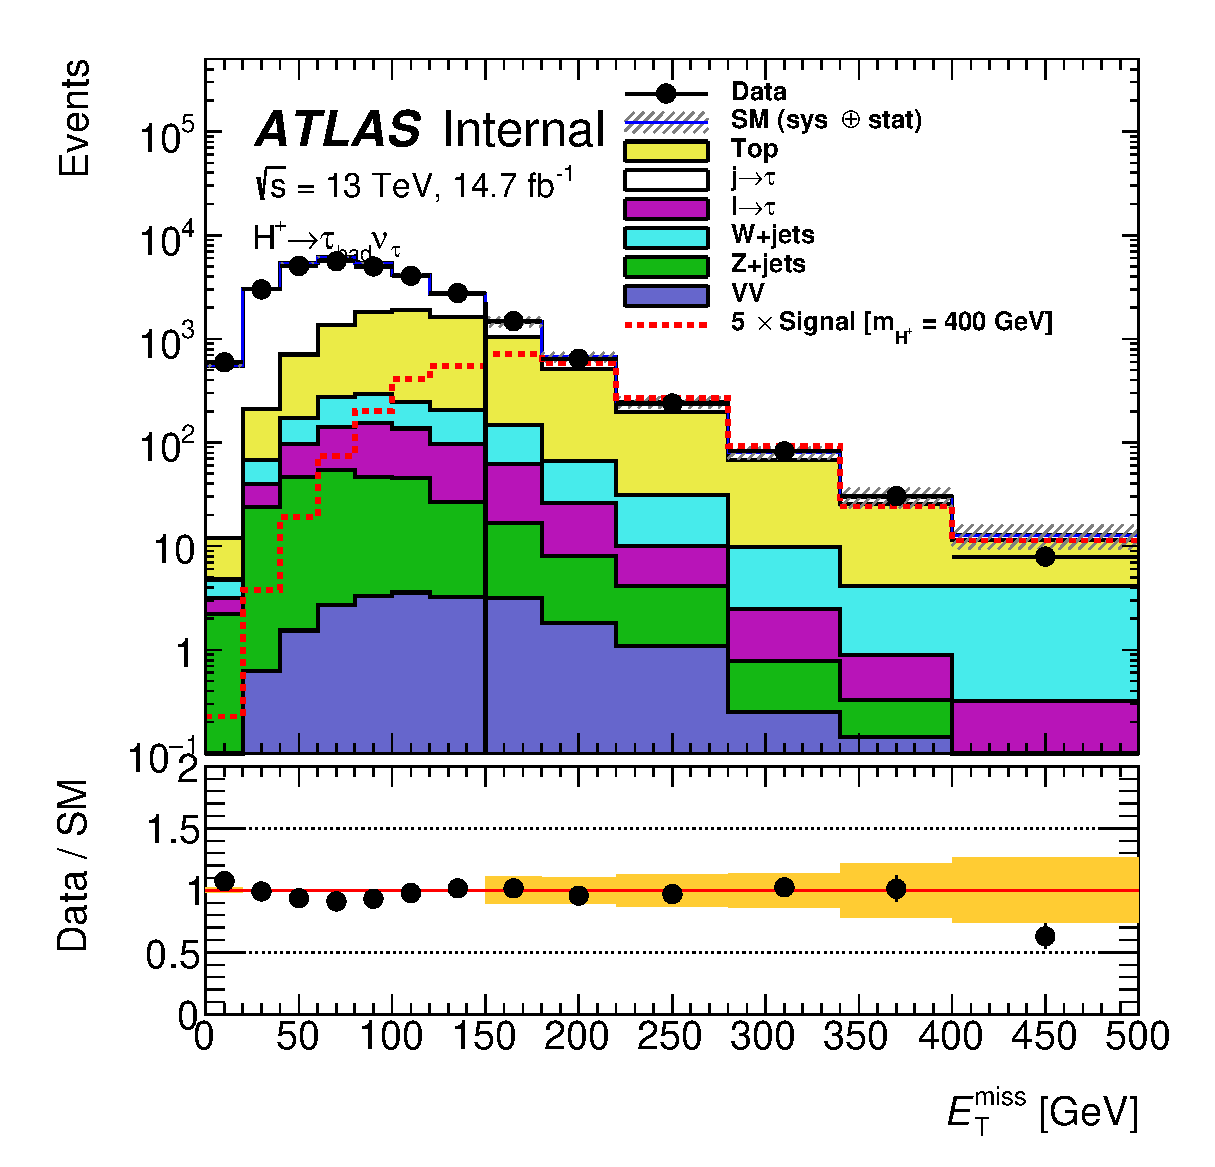
\includegraphics[width=\textwidth]{figures/met_SR_nMinus1.eps}
\caption{\met}
\end{subfigure} % 
\begin{subfigure}{0.5\textwidth}
   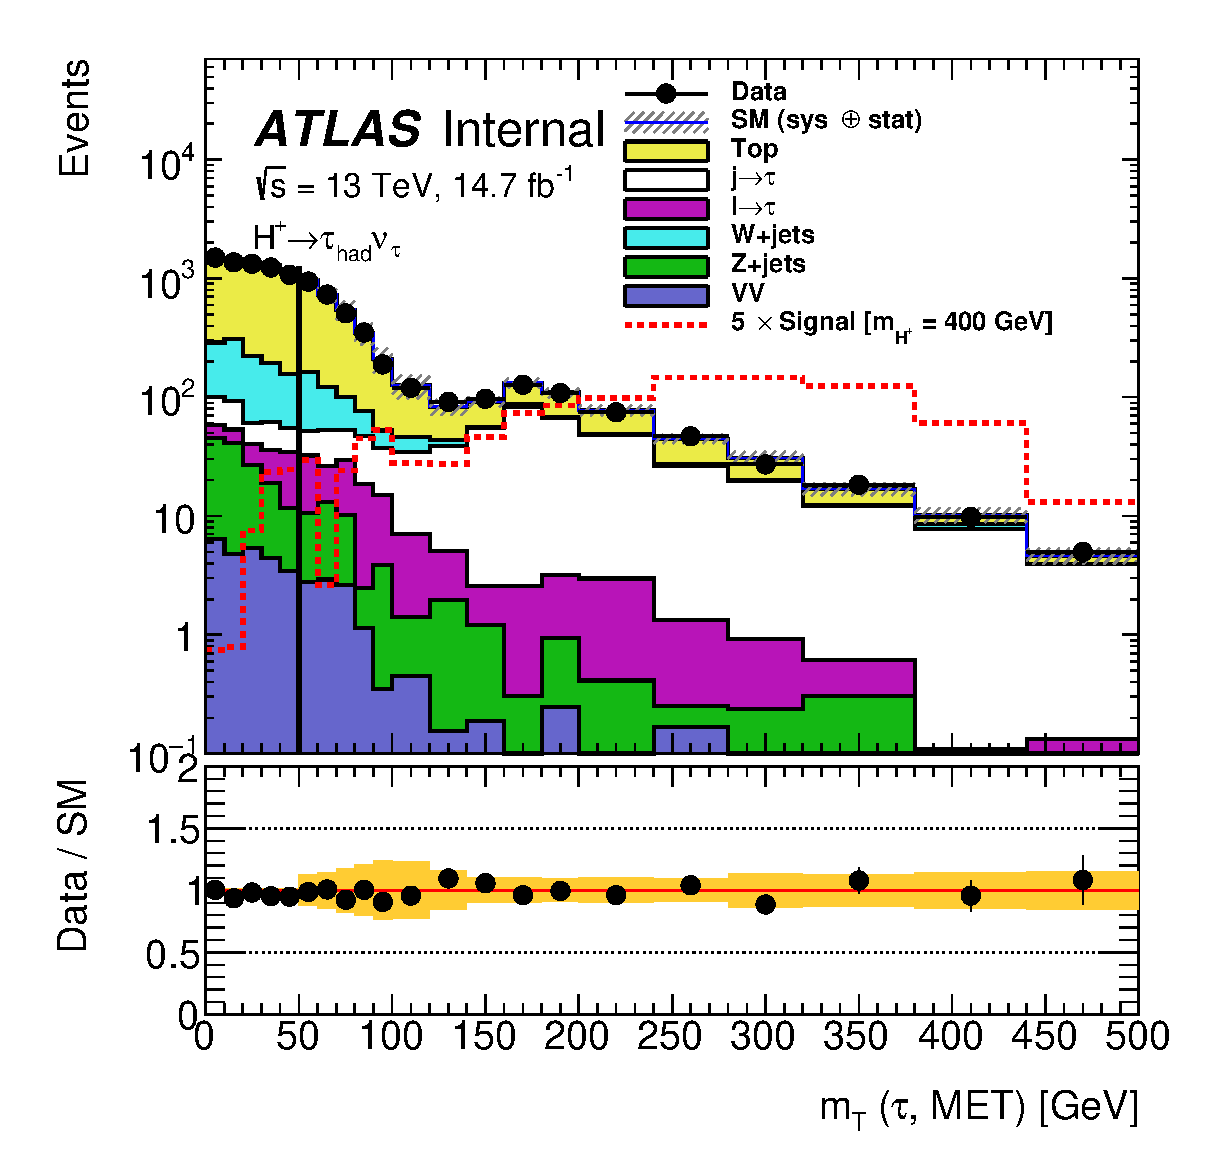
\includegraphics[width=\textwidth]{figures/mT_SR_nMinus1.eps}
\caption{\mT}
\end{subfigure}
\caption{Plots showing the \mT\ and \met\ distributions in the signal region}
\label{fig:primSR}
\end{figure}

\begin{table}[h!]
\centering
\begin{tabular}{|l|r|r|}
\hline
Category & Source & Event Yield \\
\hline\hline
\multirow{4}{*}{True \tauvis} & \ttbar\ + Single Top & 2880$\pm$770$\pm$25 \\
															& $W\to\tau\nu$        & 265$\pm$51$\pm$18   \\
															& $Z\to\tau\tau$       & 44.3$\pm$7.1$\pm$7.6 \\
															& $VV$								 & 13.8$\pm$2.2$\pm$1.7 \\ 
\hline
$j\to\tau$										& All processes				 & 1170$\pm$110$\pm$16 \\
$l\to\tau$										& All processes 			 & 126$\pm$25$\pm$6.5  \\
\hline
	Total Background						&      & 4500$\pm$779$\pm$36.4 \\				
Data (14.7~\ifb)							&											 & 4645   \\
\hline
\end{tabular}
\caption{Expected event yields in the signal region, compared to observed event yields from data.}
\label{tab:yieldsSR}
\end{table}

\par Figures~\ref{fig:secSRa} and~\ref{fig:secSRb} show distributions of other kinematic variables 
in the signal region. These are the $\pt,\eta,\phi$ of the $\tauvis$ , the number of reconstructed jets, the number 
of $b$-tagged reconstructed jets and the $\Delta\phi(\tau,\met)$. All these figures show that the 
\ttbar\ background with true \tauvis\ is the most dominant. 

\begin{figure}[!h]
\begin{subfigure}{0.5\textwidth}
					 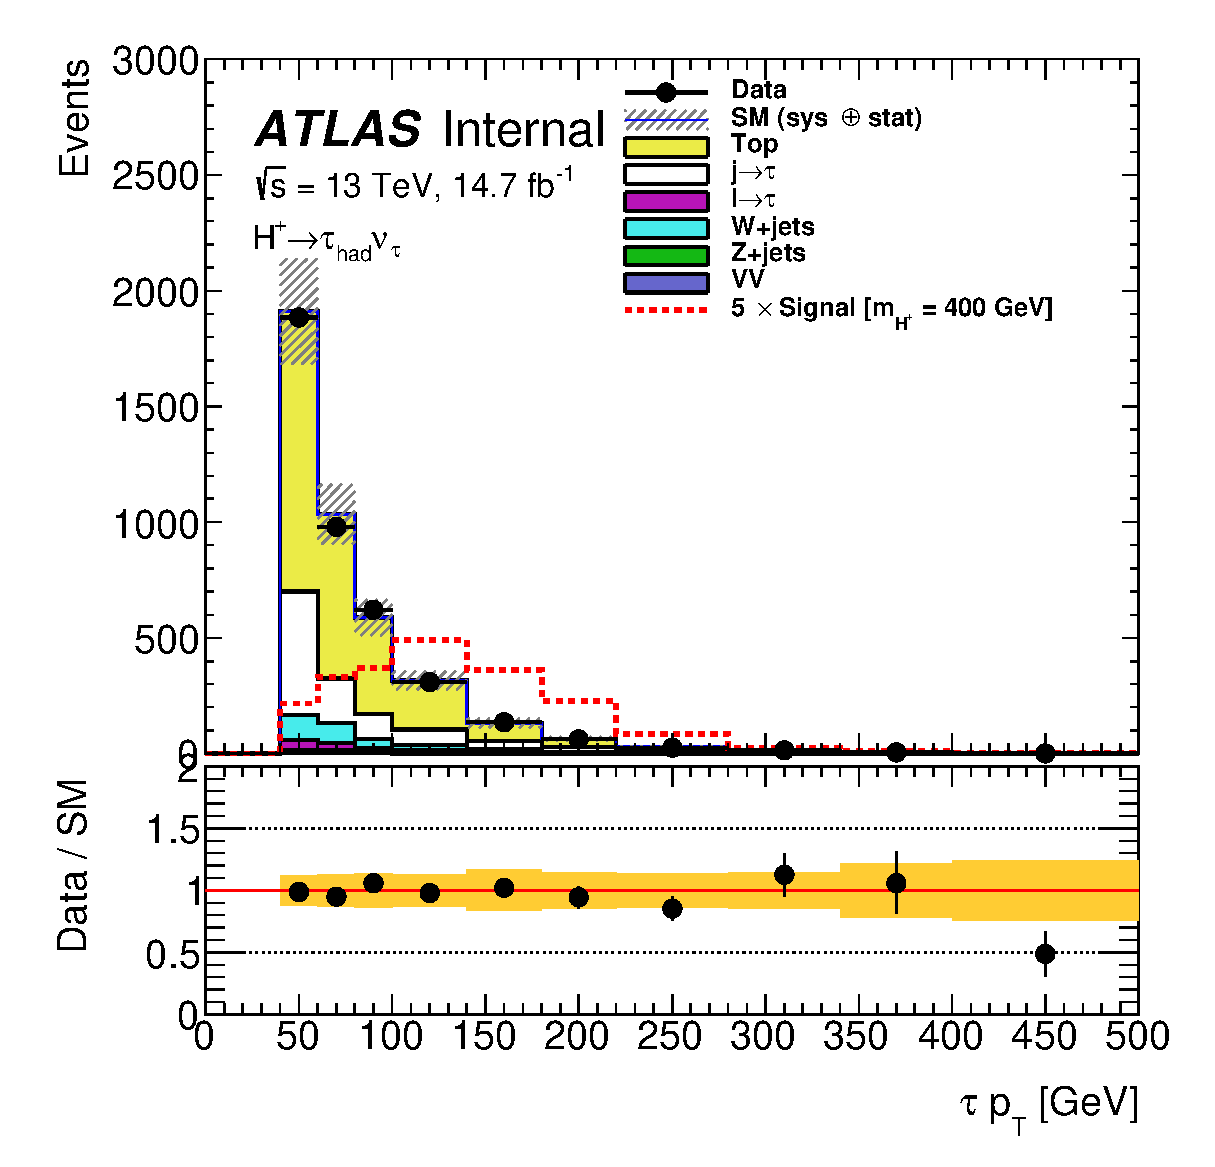
\includegraphics[width=\textwidth]{figures/tauPt_SR.eps}
\end{subfigure}  
\begin{subfigure}{0.5\textwidth}
   \includegraphics[width=\textwidth]{figures/jets_SR.eps}
\end{subfigure}
\begin{subfigure}{0.5\textwidth}
   \includegraphics[width=\textwidth]{figures/bJets_SR.eps}
\end{subfigure} %\\
\begin{subfigure}{0.5\textwidth}
   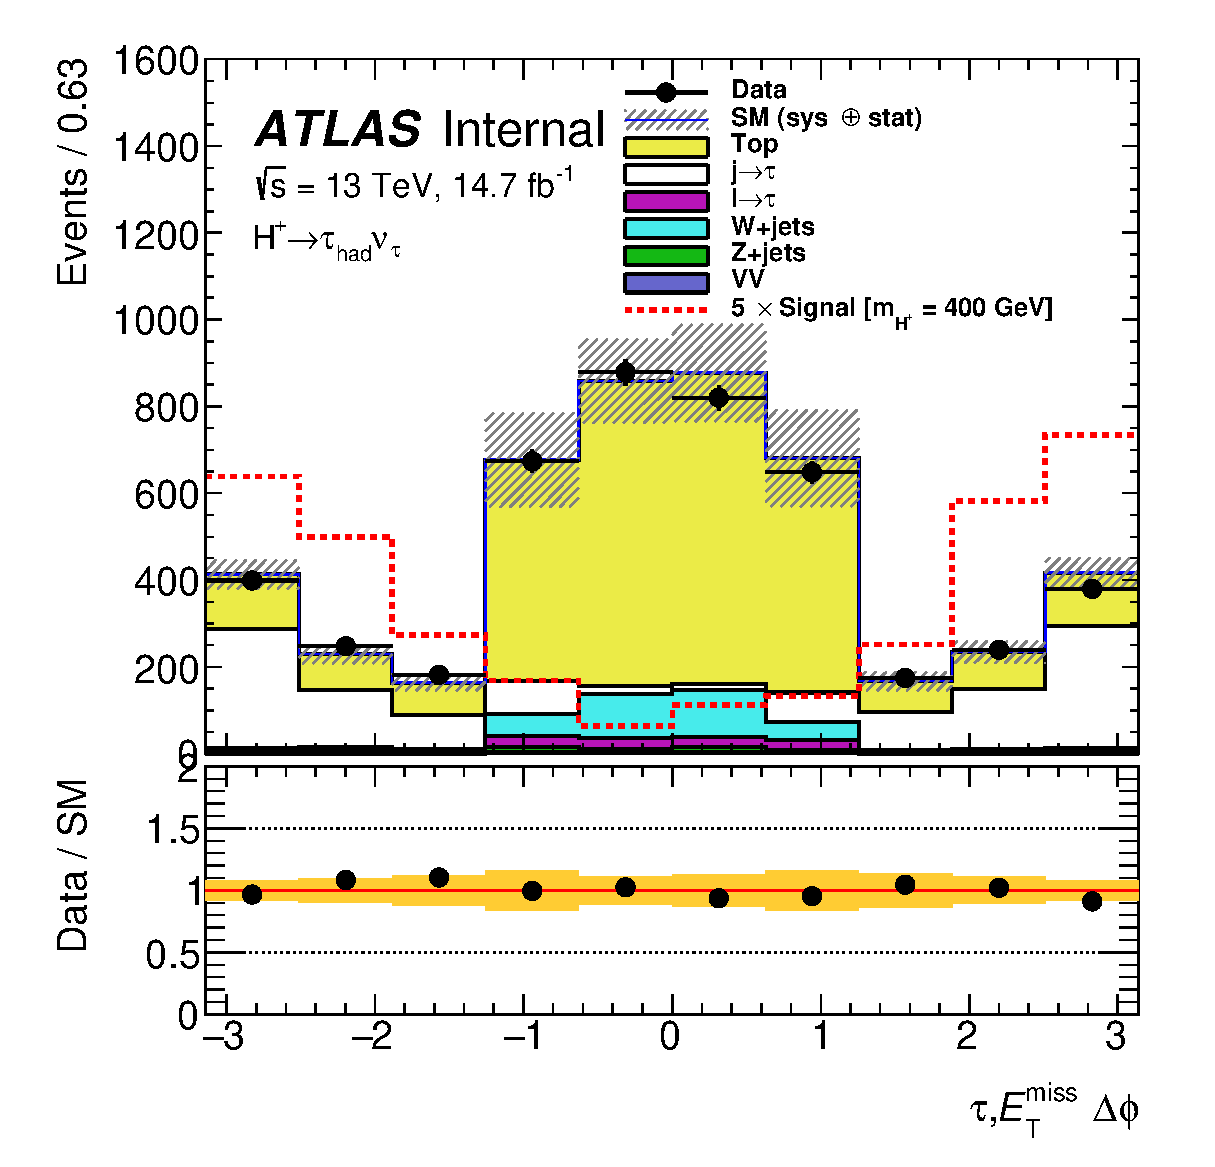
\includegraphics[width=\textwidth]{figures/tauMetPhi_SR.eps}
\end{subfigure}
\caption{Plots showing distributions of \tauvis\ \pt, number of reconstructed 
jets, number of b-tagged jets and the angular separation between the \tauvis\ and \met, 
 in the signal region}
\label{fig:secSRa}
\end{figure}

\begin{figure}[!h]
\begin{subfigure}{0.5\textwidth}
   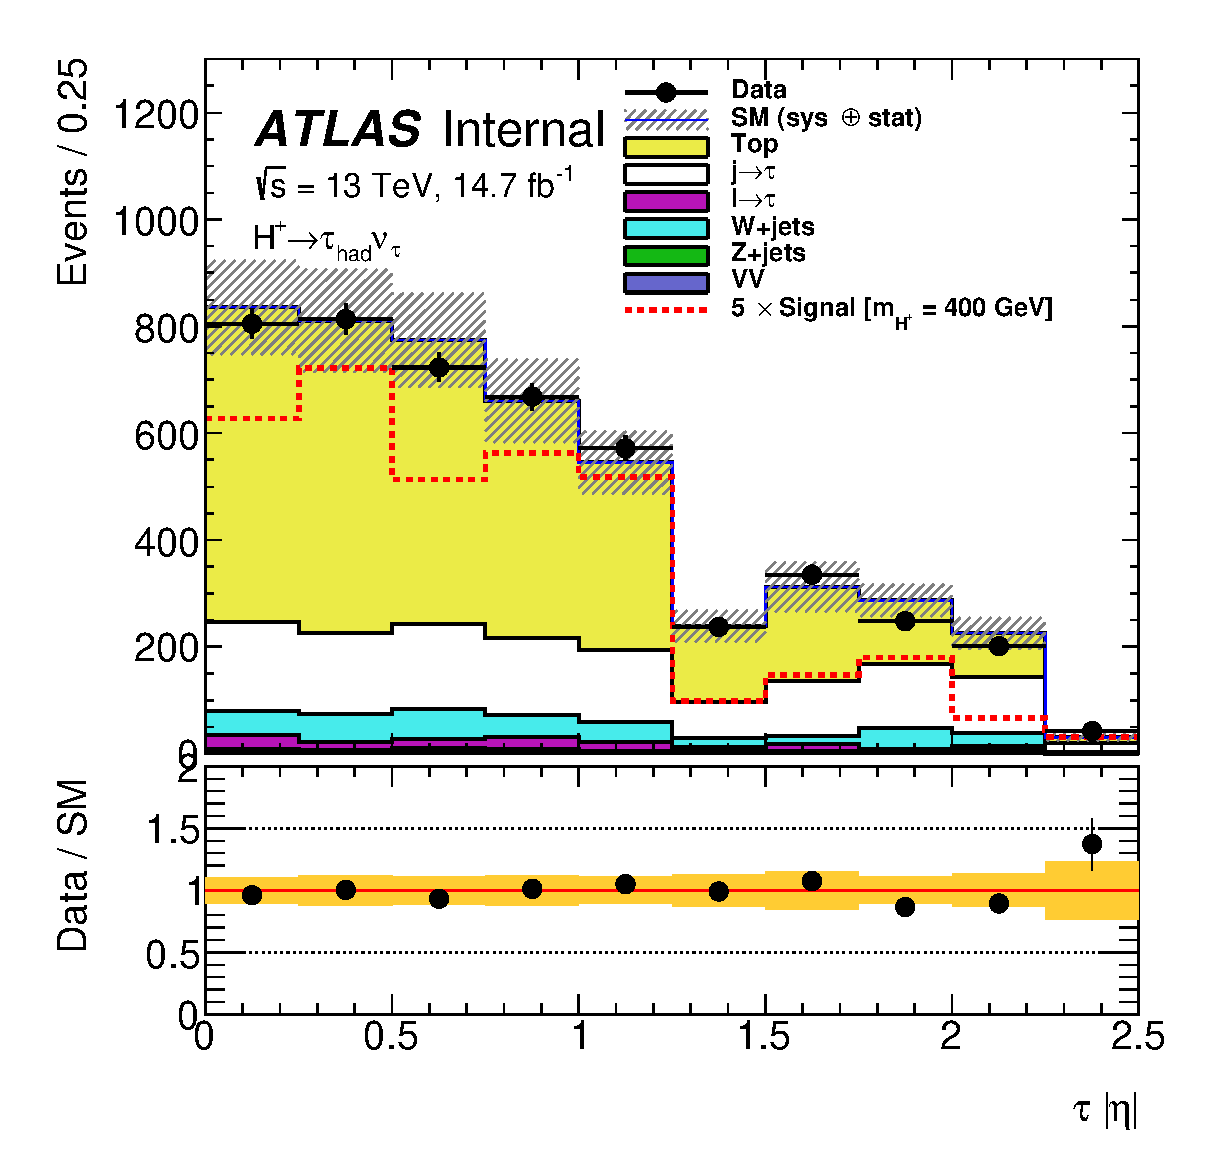
\includegraphics[width=\textwidth]{figures/tauEta_SR.eps}
\end{subfigure}
\begin{subfigure}{0.5\textwidth}
   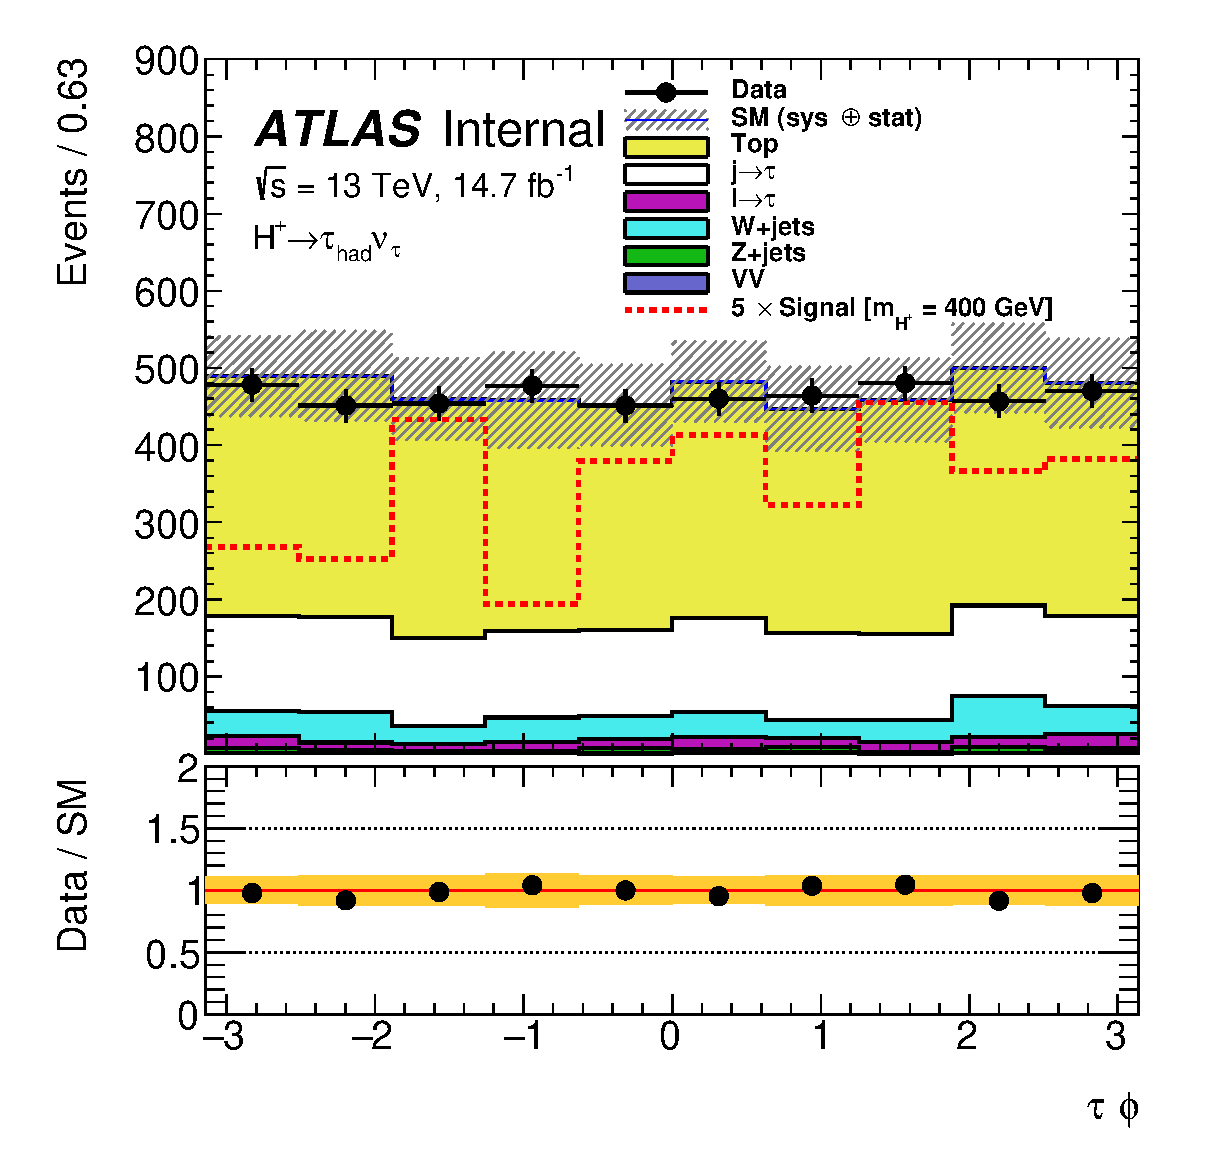
\includegraphics[width=\textwidth]{figures/tauPhi_SR.eps}
\end{subfigure}
\caption{Plots showing distributions of \tauvis\ $\eta$ and $\phi$ in the signal region}
\label{fig:secSRb}
\end{figure}

\subsection{Statistical Analysis}
\label{sec:chStat}
\par Results were tested for evidence of existence of charged Higgs bosons with $\mcH$ ranging 
from 200$\to$2000~\GeV. For each of the mass points, $\sigma^{Exp}_{H^+}$ was set at 
1 to make the parameter of interest $\mu=\sigma^{Obs}_{H^+}$. Here, the said cross section is 
the product of the production cross section and branching ratio of the topologies introduced in 
Equations~\ref{eq:topA} and~\ref{eq:topB}. The test statistic $q_0$, where $\mu=0$ 
in Equation~\ref{eq:testStat}, was used to test the compatibility 
of observed data with the background-only hypothesis. The probability distribution function 
$f(q|b)$ was estimated using the asymptotic approximation~\cite{Cowan:2010js} which 
supposes an artificial data-set called the `Asimov data-set'.\footnote{This data-set is 
defined such that if used to evaluate estimators of all parameters, true values of those 
parameters are obtained}   

\par The systematic uncertainties discussed in 
Section~\ref{sec:systsUnc} were included as nuisance parameters. 
Table~\ref{tab:nuisance_par} shows the list of all such uncertainties and 
the processes (components) to which they were applied. Those that affect more than one 
component were treated as correlated or anti-correlated, whichever was applicable. Otherwise, 
it was assummed that they were uncorrelated. Those whose 
impact on the expected event yield or \mT\ shape is less than 0.5\% were removed from the list.   
The $\pm1\sigma$ variations were symmetrized by taking the one with the largest impact on 
the result, unless there was an explicit reason for an asymmetry.  

\begin{table}[!htb]
 \begin{center}
   \footnotesize
   \begin{tabular}{l p{5cm}|c|ccc}
     {}  &  & signal & true $\tau$ & $j\ra\tau$& $l\ra\tau$ \\
     {}  &  &        & (MC)        & (Data)       & (MC) \\
     \multicolumn{2}{l|}{Contribution to total background (\%)}  &  & 72 &  25 & 3  \\
      \hline \hline            
      NUIP                          & Description &&&&\\
      alpha\_xxx &&&&&\\
      \hline
      JET\_Globally-reduced\_X     & jet energy scale: 19 components       & \ding{51} & \ding{51}  &   \ding{51} &  \ding{51} \\
     JET\_Flavor\_X               & jet energy scale: 3 components  & \ding{51} & \ding{51}  &   \ding{51} &  \ding{51} \\
     JET\_JER\_NP\_X              & jet energy resolution: 8 components  & \ding{51} & \ding{51}  &   \ding{55} &  \ding{51} \\
     TAUS\_TRUEHADTAU\_SME\_TES   & $\tauvis$ energy scale: 3 components    & \ding{51} & \ding{51}  &   \ding{55} & \\
     bjet\_xyz                     & $b$-jet identification SFs: 6 b, 4 c and 10 light components
                                   & \ding{51} & \ding{51} & \ding{51} & \ding{51} \\
     MET\_SoftTrk\_xyz            & $\met$ soft term: 2 resolution, 1 scale component
                                   & \ding{51} &\ding{51} & \ding{55} &\ding{51} \\
     met\_xyz                      & $\met$ trigger efficiency measurement: 3 components
                                   & \ding{51} &\ding{51} & \ding{55} &\ding{51} \\
     signal\_xyz                   & theoretical uncertainty on signal acceptance: QCD scale and PSUE
                                   & \ding{51} & & & \\
     ttbar\_xzy                    & theoretical uncertainty on \ttbar~acceptance and \mT~shape: scale, PSUE, ME    
                                   & &\ding{51} & &\\
     ttbar\_norm                   & \ttbar~cross section
                                   & &\ding{51} & &\\
     UWSF                          & $W\ra\tau\nu$ scale factor uncertainty
                                   & &\ding{51} & &\\
     lep\_sf                       & $\ell\rightarrow\tauvis$ scale factor  
                                   & & & & \ding{51} \\
     tau\_ID                       & $\tauvis$ identification: 2 components (all and high \pt)
                                   & \ding{51} & \ding{51} & \ding{51} & \\
     tau\_RECO                     & $\tauvis$ reconstruction efficiency
                                   & \ding{51} & \ding{51} & \ding{51} & \\
     tau\_ELEOLR                   & $\tauvis$/electron overlap removal        & \ding{51} & \ding{51} & \ding{51} & \\
     tau\_ff\_stat                 & statistics in FF method                      &  &  & \ding{51} & \\
     tau\_ff\_bdt                 & jet composition in FF method                 &  &  & \ding{51} & \\
     tau\_ff\_prompt\_tau          & mis-id prompt $\tauvis$ modelling in MC            &  &  & \ding{51} & \\
   \end{tabular}
 \end{center}
 \caption{
   Description of each of the nuisance parameters, along with
   the samples they were applied to.  If the same nuisance parameter
   was applied to different backgrounds, all correlations were kept. 
 A '\ding{51}' indicates that the systematic uncertainty was considered and included in the fit. A
   '\ding{55}' indicates that the systematic uncertainty was considered but not included in the fit, otherwise
   the given systematic uncertainty is not applied to the given background.}
\label{tab:nuisance_par}
\end{table}

\par The test of the observed data against the background-only hypothesis shows that the data 
is consistent with the Standard Model prediction. Hence, exclusion limits on  
$\mu=\sigma^{Obs}_{H^+}$ were set by rejecting the $s+b$ hypothesis at 95\% confidence 
level using the $CL_s$ procedure, where $CL_s(\mu)$ is defined as in Equation~\ref{eq:cls}.
Expected exclusion limits were computed assuming the $s+b$ hypothesis, and using the artificial 
Asimov data-set which was approximated by the sum of all the expected backgrounds. Observed 
exclusion limits are computed using the $s+b$ hypothesis, and using the total observed 
data. Figures~\ref{fig:exclLimA} and~\ref{fig:exclLimB} show the expected and observed exclusion limits for \mcH\ ranging 
from 200$\to$2000~\GeV. In the former figure, systematic uncertainties were not included in the computation 
of the exclusion limits. In the latter, the systematic uncertainties were included. 
The solid line denotes the observed limits and the dashed line denotes 
the expected limits at 95\% confidence levels. The green and yellow shaded regions represent the 
$\pm1\sigma$ and $\pm2\sigma$ uncertainty bands respectively. An illustrative signal prediction in 
the hMSSM benchmark scenario at $\tan\beta=60$ is also overlayed. Without systematic 
uncertainties the limits are slightly more stringent than with systematic uncertainties.	 
Figure~\ref{fig:exclLimB} shows that the \mcH\ range from 200$\to$540~\GeV for 
$\tan\beta=60$ is excluded by these observed exclusion limits. 

\begin{figure}[!h]
\centering
					 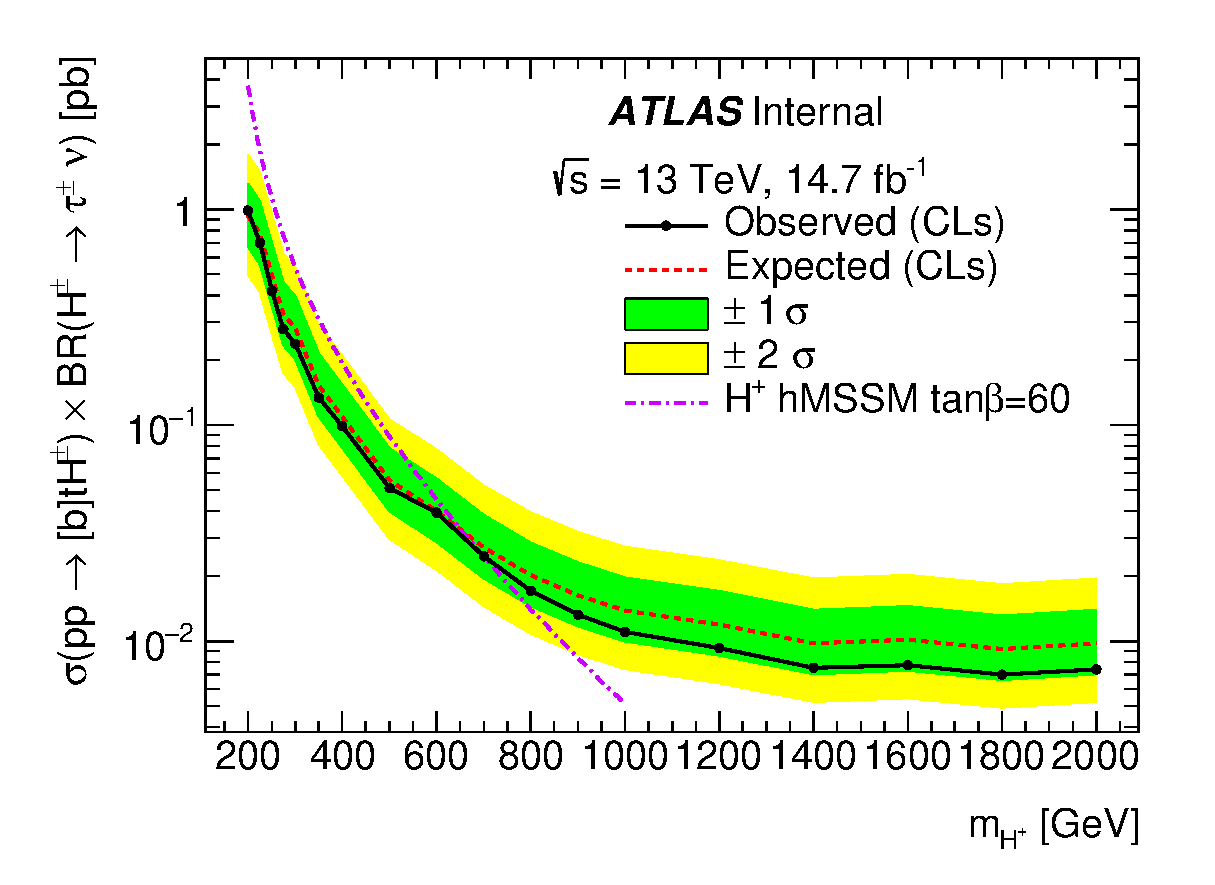
\includegraphics[width=0.8\textwidth]{figures/final_limits_no_sys_asym_limit_log.eps}
\caption{Plots of the expected and observed limits on $\mu=\sigma^{Obs}_{H^+}$, without including systematic uncertainties in the 
background and signal predictions}
\label{fig:exclLimA}
\end{figure}  

\begin{figure}[!h]
\centering
					 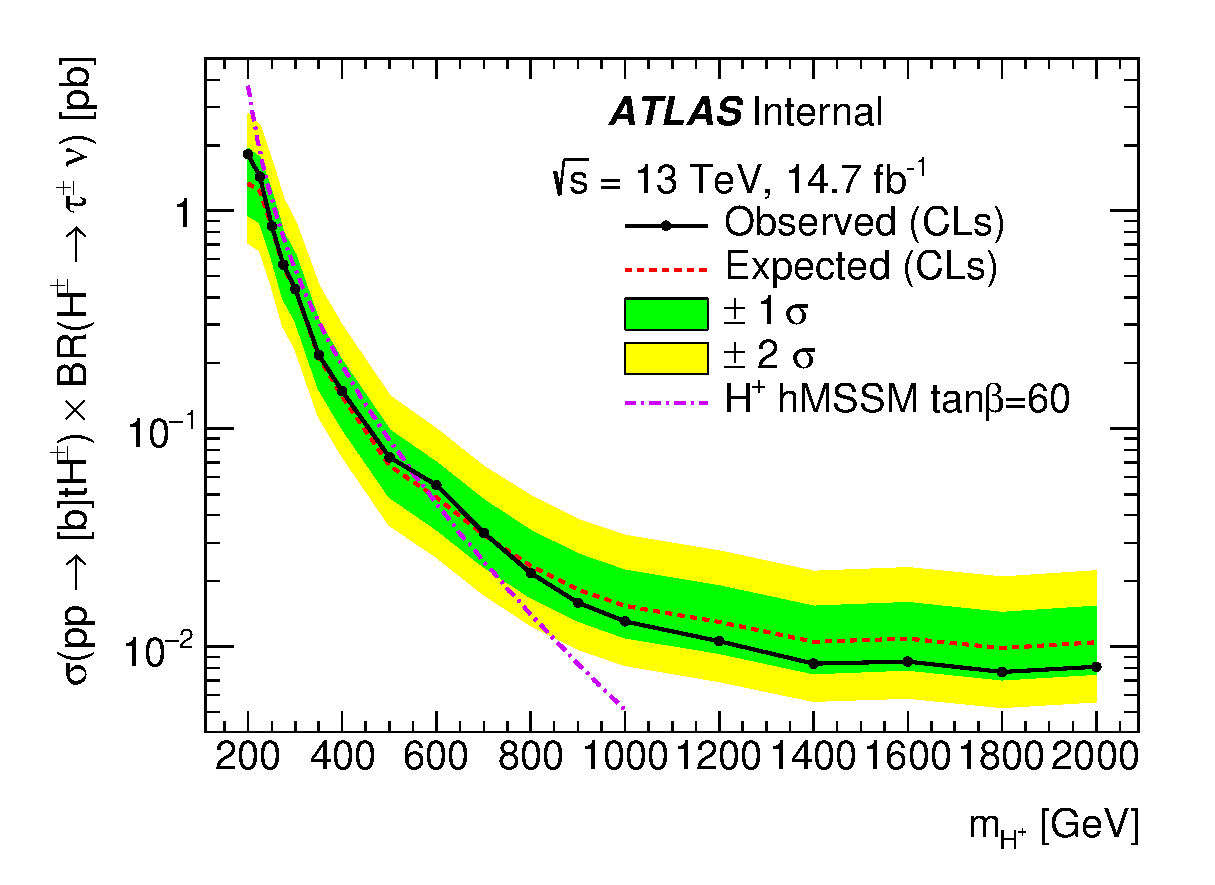
\includegraphics[width=0.8\textwidth]{figures/final_limits_sys_asym_limit_log.eps}
\caption{Plots of the expected and observed limits on $\mu=\sigma^{Obs}_{H^+}$. Systematic uncertainties were included  
in the background and signal predictions}
\label{fig:exclLimB}
\end{figure}

\par To evaluate the impact of the individual limits on exclusion limits shown in Figure~\ref{fig:exclLimB} 
the limit-setting procedure was repeatedly performed without including each of the systematic 
uncertainties. Table~\ref{tab:syst_taujets_postfit} summarizes the impacts of groups of these 
systematic uncertainties for $\mcH=200~\GeV$ and $\mcH=1~\TeV$. The percentage impact was obtained 
by comparing the nominal expected limit and the expected limit computed without considering each of 
these groups of uncertainties. Evidently, the largest impact is from fake factos and \ttbar\ background 
modelling.    

\begin{table}[h!]
 \begin{center}
  \resizebox{\textwidth}{!}{
   \begin{tabular}{|l|l|cc|}
\hline
Category    &  Source of systematic & \multicolumn{2}{c|}{Impact on the expected limit (in \%)} \\
    &  uncertainty & $m_{H^+} = 200~\GeV$ & $m_{H^+} = 1000~\GeV$ \\
     \hline\hline
	\multirow{5}{*}{Experimental} & luminosity  &  $\phantom{0}1.5$   &  $\phantom{0}0.9$ \\
     & trigger  &  $<0.1$  &  $<0.1$ \\
     & $\tau_{\text{had-vis}}$  &  $\phantom{0}1.0$   &  $\phantom{0}1.4$ \\
     & jet  &  $\phantom{0}3.0$   &  $\phantom{0}0.2$ \\
     & $\met$  &  $<0.1$   &  $<0.1$ \\
     \hline
 \multirow{1}{*}{Fake factors} &  \FF  &  $\phantom{0}0.8$   &  $\phantom{0}4.7$ \\
     \hline
 \multirow{2}{*}{Signal and background models}    & $t\bar{t}$ modelling   &  $\phantom{0}13.2$   &  $\phantom{0}3.5$ \\
     & $H^+$ signal modelling  &  $\phantom{0}1.4$   &  $\phantom{0}1.4$ \\
     \hline
   \end{tabular}
}
   \caption{Impact of various sources of uncertainty on
      the expected 95\% CL exclusion limit.}
\label{tab:syst_taujets_postfit}
  \end{center}
\end{table}


%
%\begin{chapsummary}
%A search for evidence of the charged Higgs boson in the decay 
%channel $H^+\to\tau\nu$, in association with a top quark, was performed in 14.7~\ifb 
%of $pp$ collision data collected by the ATLAS detector. The data was found to be 
%consistent with the Standard Model prediction, as opposed to the hMSSM model presented 
%in Chapter~\ref{theory}. Exclusion limits were set on the product of the production 
%cross section of the charged Higgs boson and the branching ratio of its decay to a 
%$\tau$ lepton and a $\nu_\tau$, for charged Higgs boson masses in the range 200$\to$2000~\GeV. 
%In the hMSSM context, $\tan\beta=60$ values are excluded for the charged Higgs boson 
%mass range $200\to 540~\GeV$. As the ATLAS detector keeps on collecting more data, 
%results for this search keep on evolving. 	  
%\end{chapsummary}
